%
%  normalEstimators
%
%  Created by Daniel Beatty on 2007-10-19.
%  Copyright (c) 2007 Texas Tech University. All rights reserved.
%
\documentclass[11pt]{article}
\usepackage{geometry}                % See geometry.pdf to learn the layout options. There are lots.
\geometry{letterpaper}                   % ... or a4paper or a5paper or ... 
%\geometry{landscape}                % Activate for for rotated page geometry
%\usepackage[parfill]{parskip}    % Activate to begin paragraphs with an empty line rather than an indent
\usepackage{doublespace}
\usepackage{graphicx}
\usepackage{amssymb}
\usepackage{epstopdf}
\usepackage{listings}

\usepackage{algorithm,algorithmic}
\DeclareGraphicsRule{.tif}{png}{.png}{`convert #1 `dirname #1`/`basename #1 .tif`.png}

\newtheorem{thm}{Theorem}[section]
\newtheorem{adef}[thm]{Definition}
\newtheorem{cor}[thm]{Corollary}
\newtheorem{lem}[thm]{Lemma}

\title{Normal Classifiers using Mathematica, Octave, and Core Graphics}
\author{Dan Beatty}
%\date{}                                           % Activate to display a given date or no date

\begin{document}
\maketitle
%\section{}
%\subsection{}

\section{Introduction}
In the original two assignments for the pattern recognition course, the class was instructed to explore four algorithms: Principal Component Analysis (PCA), Multiple Discriminant Analysis (MDA), Expected Maximization(EM), and Independent Component Analysis (ICA).  PCA, MDA, and EM  are described in the mathematical overview section (section \ref{math-overview-section}).  ICA is given its own section as this algorithm is commonly misunderstood and clarification is warranted to understand the work presented in this report.  

The specific assignment for EM, PCA, and MDA is stated as follows:
\begin{quote}
\begin{itemize}

	\item You are given a total of 150 four dimensional samples of three Iris species.  Use Multiple Discriminant Analysis (MDA) to separate the samples into three Iris species. Show the resulting misclassifications.   Repeat MDA choosing any three-dimensional features at a time and show the resulting misclassifications.

	\item You are given a retinal digital picture in color.  Take the gradient of the monochrome image and use the Expectation-Maximization (EM) algorithm to extract the edge points from the blurred optic disc boundary.

	\item Use Principal Component Analysis (PCA) in combination with the Whitening transform and Linear Discriminant Analysis (LDA) to classify and segment the optic disc from the background.	

\end{itemize}
\end{quote} 

For an image, segmenting any portion on the fly is a difficult thing to perform due to interface constraints.  MDA for example is complied with in a prototype manner in this report as such an interface has not been built yet.  MDA is described in theory in subsection \ref{mda-description-subsection}, and has a Mathematica prototype for the Iris species included in section \ref{mathematica-prototype-mda}.  The Mathematica version was chosen at the time since MATLAB was unavailable due to changes in platform (both Mac with Intel chips and Microsoft's Windows Vista).  Also, for the problem in question Mathematica simply seemed more intuitive for the problem at hand.   



For the EM algorithm, another two prototypes were constructed.  One of them is an Octave implementation of a classic Matlab implementation of the EM algorithm, originally by \cite{yamazaki98introduction}.  This implementation can be directly translated into C (consequently Objective-C and C++).  However, this direct translation has drawbacks to being utilized in a production system that users will expect to be responsive.  In subsection \ref{em-description-subsection}, this report describes the essence of the EM algorithm from its mathematical foundation.  In section \ref{classic-em-implementation}, the EM classic implementation is described as well as modifications to ensure responsiveness in a GUI based application.  The prototype GUI-based implementation leads to a more general form using Quartz Composer plug-ins, and yields reasonable results.

As will be pointed out in the PCA subsection (\ref{pca-sub-section}), whitening and classical estimators for PCA are nearly synonymous.  Differences between PCA and whitening only have to do with the inclusion of scaling factors, which are obtained in the process of determining the PCA estimator.

While the CPU bound prototype for PCA, written for this report (in Objective-C), is typical of other implementations of PCA (most notably MATLAB implementations), it leaves much to be desired with regards to efficiency.  The implementation in this example uses the Linear Algebra Package (LAPACK) libraries which are part of the Accelerate Framework in all Apple OSX systems since version 10.2.   Even with these libraries, the lack of use of the many processors available on the hardware the system is running on.  While this is the fastest the CPU can offer, there is another processor on the user's system that can offer.   In section \ref{pca-classic-implementation}, a CPU bound implementation is demonstrated and attempts to squeeze as much efficiency from the CPU as possible.  %This is exceedingly wasteful, and denies a swift experience for users.  In section \ref{pca-classic-implementation}, a demonstration of PCA in this form is performed by segmenting the iris image.  

%Proofed as of Nov 14

%ICA and, in particular, its primary implementation projection pursuit is another story.  While a command line solution can receive results in less than 30 seconds, that time frame is actually eternity for real-time applications.  One characteristic of projection pursuit is the size of the transformation matrix, and it is the size of this transformation matrix that allows alternative processing methods to be considered.  It is predicted that those methods, on average, will have a more acceptable real-time execution rate, which represents a considerable performance improvement. 

ICA in the form of projection pursuit can be seen as an extension of PCA.  For a single independent component, projection pursuit performs acceptably well.  However, if that algorithm were to be used in deflationary pursuit, the complexity would grow.  

The original instructions the pattern recognition class was provided for ICA read as follows:

\begin{quote}
	This project is to illustrate how a modified Independent Component Analysis (ICA) can be used to restore an image corrupted with additive Gaussian noise.  

	Choose any natural image (of a reasonable size), add 30\% Gaussian noise to the image, assuming a noisy image model:
	\begin{equation}
	\vec{z} = \vec{x} + \vec{n}
	\end{equation}
	%where include picture  \\
%	``http://www.cis.hut.fi/aapo/papers/IJCN99\_tutorial/img163.gif'', mergeFormatInet is Gaussian, and include picture \\ ``http://www.cis.hut.fi/aapo/papers/IJCNN99\_tutorialweb/img8.gif'' where mergeFormatInet is non-Gaussian.  
	
	Denoise the noisy image by using the Sparse Code Shrinkage Method (closely related to ICA) as described in the following in the following reference. 
	
	Compare the restored image using the above method with standard noise removal filters such the simple median filter or the Wiener filter. 
	
	MATLAB codes for various versions of ICA are available from the home page of A Hyv$\ddot{a}$rien and the Laboratory of Computer and Information Science at the University of Helsinki. 
\end{quote}
It turns out that the MATLAB codes provided by Hyv$\ddot{a}$rien leave much to be desired in comparison with his own book.  As such, it is typically downloaded in a broken state and is difficult to debug due to the complexity of the MATLAB codes.  The implementation of projection pursuit and deflation pursuit presented in this report is a simplification based on the algorithms found in Hyv$\ddot{a}$rien's book.   The improvements made to the implementation are covered in a separate chapter and extensively referenced in the appendix on the topics of Quartz-Composer plug-ins and Core Image Kernel Filters, which are key to the construction of the alternative form.   




\section{Mathematical Overviews}\label{math-overview-section}
Expected Maximization (EM), Linear Discriminant Analysis (LDA), and Principal Component Analysis (PCA) can each be classified as a family of estimators.  Classically known estimators %classically known  
include  least squares and maximum likelihood, %both constitute estimators which 
 which
differ by their method of convergence.  LDA is a special case of Multiple Discriminant Analysis  (MDA) where the number of discriminants is reduced to two.  

\newpage
Both PCA and MDA produce mappings of zero mean data to orthogonal vectors.   MDA differs by using both the background scatter of the entire data  and specified ``within'' scatter matrices defined by specific segments of the data.  A scatter matrix $S$ is defined in the following equation: %equation \ref{typical-scatter}:
\begin{equation}
	S = \sum _k (\vec{x_k} - \vec{m})(\vec{x_k} - \vec{m})^T \label{typical-scatter} 
\end{equation}

A background scatter matrix is the scatter matrix for the entire collection of data points.  In practice, it is more useful to determine a scatter matrix for a reasonable sampling of the data than to use the entire data set.   From such a background scatter matrix, the principal components can be determined.

\subsection{Principal Components}\label{pca-sub-section}

\begin{quote}
	The principal components of the observed data are selected so that the ith principal component is the linear combination of the observed data that accounts for the ith largest portion of the variance in the observations.
\cite[329]{moon-stirling-book}
\end{quote}

Let $\vec{x}$ be a sample from the observed data whose space is denoted $\mathbf{X}$.  Let $\vec{y}$ be the principal components of $\vec{x}$.  Then there is a transformation matrix $\mathbf{P}$ such that equation \ref{pca-characteristic} is satisfied.
\begin{equation}
\vec{y} = \mathbf{P}\vec{x} \label{pca-characteristic}
\end{equation}
In order for $\mathbf{P}$ to satisfy equation \ref{pca-characteristic},  it should maximize equation \ref{pca-optimization-definition}.  This choice is made to satisfy the least squares error.  
\begin{equation}
J(\mathbf{P}) = E\{ \vec{y}^2 \}  \label{pca-optimization-definition}
\end{equation}
Most texts show that for each column vector of $\mathbf{P}$ to have a derivation as shown in equation \ref{pca-optimization-derivation}.  The important feature of $\mathbf{P}$ to be noted is that the eigenvectors of the covariance matrix of $\mathbf{X}$ are ordered by matching eigenvalues. 
\begin{eqnarray}
J(\vec{p}_1) = E \{ y^2 _1 \} = E \{ (\vec{p}_1^T \vec{x} )^2 \} = \vec{p}_1 ^T E \{ \vec{x}\vec{x}^T \} \vec{p}_1 \label{pca-optimization-derivation} \\
 || \vec{p}_1 || = 1 
\end{eqnarray}
%Note that any 
Any $\mathbf{P}$ that satisfies the constraints of PCA is a valid PCA transformation matrix.  Some methods simply approximate $\mathbf{P}$, and are not a collection of eigenvectors.  These methods are often called on-line methods because they approximate $\mathbf{P}$ as each $\vec{x}$ becomes available. Other methods obey equation \ref{pca-optimization-derivation} by obtaining the eigenvectors, and some texts call these methods batch methods as they work on $\mathbf{X}$ as a collected whole. 
Singular Value Decomposition, Karhunen-Loeve,  Hotelling transforms, and Pearson all acquire the transformation matrix that determines the principal components.

%The purpose of PCA is  that it finds a set of orthogonal basis vectors for a collection of vectors assembled in a matrix.  The collection of these vectors allows the original data to be mapped into an orthogonal space.  There are well studied methods for obtaining principle components, such as Karhunen-Loeve \cite{} and the Singular Value Decomposition \cite{} (SVD).  While it is true that they each obtain equivalent results, how they do this determines their effectiveness.  Also, some methods have side-products that may be useful.  

In the end, the principle components are simply defined in terms of eigenvectors and  eigenvalues for a scatter matrix.  
As stated earlier in the section, the background scatter matrix can be used to determine the principal components as well.  A mixing matrix, $\mathbf{P}$, can determine each principal component as shown in equation \ref{data-by-principal-component}.   %Equation \ref{principal-component} is 
In this case, there is an assumption that each data vector $\vec{x}$ is defined in terms of some mixing matrix, $\mathbf{P}$, a matching set of principal components $\vec{a}$, and a mean vector $\vec{\mu}$.   The mean can for practical purposes be the sample mean of $\vec{x}$.  
Equation \ref{principal-component} shows the inverse relation of principal component to data vector.  %In this derivation, the columns of $\mathbf{P}$ are the eigenvectors of the scatter matrix, although any orthonormal matrix will suffice.

% In particular, the principal components can be defined by the derivation leading to the definition of a principal component in equation \ref{principal-component}.  In this derivation, the columns of $\mathbf{P}$ are the eigenvectors of the scatter matrix.  
\begin{eqnarray}
\vec{x} = \vec{\mu} + \mathbf{P}\vec{a} \label{data-by-principal-component} \\
\mathbf{P}^T(\vec{x} -\vec{\mu}) = \vec{a} \label{principal-component} \\
\vec{x} = \vec{\mu} + \sum _i a_i \vec{e_i} \label{data-by-principal-component-eigenvector} 
\end{eqnarray}

%The eigenvectors of the scatter matrix also belong to the columns of the $\mathbf{V}$ matrix of the SVD defined by $\mathbf{A} = \mathbf{U\Lambda V}^T$.  Likewise, the eigenvalues of the scatter matrix are part of the diagonal matrix $\Lambda$.  The renaissance framework includes a wrapper to the LAPACK implementation of SVD, and is a logical choice for computing PCA through the Central Processing Unit (CPU). %Since the SVD is part of the LAPACK, the renaissance libraries us wrappers of the dcgRenaissance, this logical choice of implementation for acquiring the SVD.  

%As will be shown in another report, 
Principal components are can be used %necessary often used for 
determining the independent components.  The reason is that principal components inherently possess properties zero mean and of unit variance.  Also, as defined in equation \ref{data-by-principal-component-eigenvector}, order of the eigenvectors are irrelevant.  %One thing of note,
It is important to ensure that the eigenvectors are orthonormal for this derivation and equation \ref{data-by-principal-component-eigenvector} to be correct.  Some eigenvector estimators compute the eigenvectors but without any form of normalization.  The result of failing to ensure normality is a scaled version of the principal components, which is wrong.  


For CPU bound computation of PCA, SVD is a classic well known algorithm that is part of the LAPACK libraries and has  acceleration via the Accelerate framework \cite{apple-accelerate-framework}.  For GPU bound, both classic methods and online methods should be considered.  At the time this report was written, only a scant number of implementations of PCA were made for the GPU.  Of those made, all of them were constructed for this report.  Those considerations at this time are beyond the scope of this report. 

In section \ref{transformation-masking-maps}, PCA and Independent Component Analysis (ICA) are explored in the perspective of how to apply them image processing, filters and masks.  In the context of masks, it is more convenient to use the transformation matrix% and use it 
in the construction of a filter.  In some filtering processes, it is better to use the principal components, and the inverse mixing matrix.

The following two subsection describe both Eigenvector Decomposition (EVD) and Gram-Schmidt Orthogonalization (GSO).  Both procedures are well known methods for obtaining an orthogonal matrix, which will satisfy the mixing matrix.  EVD is included in LAPACK, and already has a CPU bound implementation which has been optimized via the Accelerate Framework.  GSO is better candidate for GPU bound computations as it can be constructed via modules that are zero-branch.


\subsubsection{Gram-Schmidt Orthogonalization}
Principal components are defined by a transformation matrix which is orthonormal and typically consisting of eigenvectors.  One other estimate for such an orthogonal matrix is called Gram Schimidt Orthogonalization (GSO).   %One single theorem forms the basis for GSO.
%One significant operation object handles the Gram Schmidt Orthogonalization.  
%An example of classes designed to work on DCGMatrix is class named DCG-Gram Schmidt Orthogonalization (DCGGramSchmidt).   
Theorem \ref{gso-theorem} states that an vector space $\mathbf{V}$ can be transformed in to another vector space $\mathbf{W}$ such that each $\vec{w}\in \mathbf{W}$ is orthogonal.  GSO is a procedure based on theorem \ref{gso-theorem} that constructs each $\vec{w}_i \in \mathbf{W}$ one right after the other, and is defined in algorithm \ref{alg:gso}.
%As stated in theorem \ref{}, the goal of this class is to construct Gram Schmidt orthogonalization of a matrix consisting of column wise vectors.  The result is also a column wise matrix whose columns are orthogonal to one another.   

\begin{quote}
\begin{thm} 
\label{gso-theorem}
Suppose $w_1, w_2, ..., w_n$ form an orthogonal set of non-zero vector in $\mathbf{V}$.  Let $v$ be any vector s.t. $v \in \mathbf{V}$.  Define $v'$ s.t. 
\begin{eqnarray}
v' = v - c_1 w_1 - c_2 w_2 - ... - c_n w_n \\
c_i = \frac{\langle v , w_i \rangle} {||w_i||^2}
\end{eqnarray}
Then $v'$ is orthogonal to $w_1, w_2, ..., w_n$.
\end{thm} \cite[211]{schaums-linear-algebra}
\end{quote}


\begin{algorithm}
\caption{Gram Schmidt Orthogonalization}
\label{alg:gso}
\begin{algorithmic}
	\REQUIRE Column Wise Source Matrix: $\mathcal{V}$
	\STATE $N$ is the number of column vectors in $\mathcal{V}$
	\STATE Base case $\vec{v}_0 = \vec{w}_0$ 
	\STATE initialize $\vec{\theta}^0$, $T$, and $i \leftarrow 0$
	\STATE $v_0 \leftarrow $ [V columnVector:1]
	\STATE [W insertVector:$v_0$ atColumn:1]
	\FOR {j = 2 to N}
		\STATE $v_j \leftarrow$ [V columnVector:j]
		\FOR {i = 1 to j}
			\STATE $(w_i)_{\textsl{norm}} \leftarrow ||w_i ||$  
			\STATE innerProduct ($i_p$)$\leftarrow$ $\langle w_i , v_j \rangle$
			\STATE \textsl{negsum} += $i_p / (w_i)_{\textsl{norm}}$
		\ENDFOR
		\STATE result = $v_j - \textsl{negsum}$
		\STATE [W insertVector:result atColumn:j]
	\ENDFOR
	\RETURN $W$
\end{algorithmic}
\end{algorithm}

\subsubsection{Eigenvalues: Characteristic Polynomials}
\begin{quote}
	\begin{adef}
		Consider an $n$-squared matrix $\mathbf{A}$ over a field $\mathcal{K}$
		\begin{equation}
			\mathbf{A} = 
			\left(
			\begin{array}{cccc}
				a_{11}  &a_{12}  & ... &a_{1n}     \\
				a_{21}  &a_{22}  & ... &a_{2n}     \\
				...& ...& ...&... \\
				a_{n1}  &a_{n2}  & ... &a_{nn}     \\
			\end{array}
			\right)
		\end{equation}
		The matrix $t\mathbf{I}_n - \mathbf{A}$ where $\mathbf{I}_n$ is the $n$-square identity matrix and $t$ is an intermediate, is called characteristic matrix of $\mathbf{A}$
	\end{adef}
	\cite[281]{schaums-linear-algebra}
\end{quote}
The determinant of the characteristic matrix is the characteristic equation (polynomial) of $\mathbf{A}$.  The definition for eigenvalues and eigenvectors is stated in the quoted definition \ref{eigenvalueDefinition}.
\begin{quote}
\begin{adef}
	\label{eigenvalueDefinition}
Let $\mathbf{A}$ be an $n$-square matrix over a field $\mathcal{K}$.  A scalar $\lambda \in K$ is called an eigenvalue of $\mathbf{A}$ if there exists a nonzero (column) vector $\vec{v}\in \mathcal{K}^n$ for which equation \ref{eigenvalueCharacteristicEquation} holds.
\begin{equation}
\mathbf{A}\vec{v} = \lambda \vec{v}  \label{eigenvalueCharacteristicEquation}
\end{equation}
Every vector satisfying this relation is then called an eigenvector of $\mathbf{A}$ belonging to the eigenvalue $\lambda$.
\end{adef}
\cite[284]{schaums-linear-algebra}
\end{quote}
There is a family of algorithms called Eigenvalue Decomposition (EVD) that finds the eigenvalues and eigenvectors.   EVD is part of the Linear Algebra Package (LAPACK) libraries and consequently part of the Accelerate framework\cite{apple-accelerate-framework}.  Thus for CPU bound operations, the LAPACK version is the best choice, as it is already optimized for the CPU.    %There are reasons to consider EVD algorithms in the GPU bound case, as none exist at the time of this report.   


%\subsubsection{Principle Components}   
%
%There are classical means for obtaining the transformation that satisfies the principal components.   %Each column vector of the transformation matrix is an eigenvector of the covariance matrix, and the order is determined by size of corresponding eigenvalue.  

%There are both classical methods (often called batch methods),  and ``on-line'' methods (methods that converge on the solution via neural network ``learning'').  




\subsection{Multiple Discriminant Analysis}
\label{mda-description-subsection}
A ``within'' scatter matrix for each category uses selected data points $\vec{x_s}$  that are believed to be within a specific category.  Each category's scatter matrix, $\mathbf{S_i}$ is summed to form the within scatter matrix $\mathbf{S_w}$, as in equation \ref{total-within-scatter-matrix}.  There is one presumption about the data that must be taken into account regarding these types of scatter matrices, namely size. 
\begin{equation}
	S_w = \sum_i S_i \label{total-within-scatter-matrix}
\end{equation}
In terms of image processing, this selecting member data vectors $\vec{x_i}$ %selection 
is not as trivial or randoms as is the case for principal component analysis.  The size of this scatter matrix must %still 
be the same as the background scatter matrix.  If it were, the columns or rows that were specific attributes to be extracted would be viable.  Consequently, the size of each $\vec{x}$ is the length of a column in the image.  Another approach is to use neighborhood vectors as discussed in section \ref{sparse-coding-shrinkage}.  In the case of neighborhood vectors, the characteristic the background scatter matrix should be composed of a random set of neighborhoods union any members composing the within scatter matrix.  
%If the specific region used to construct the within scatter matrix is smaller, then the background scatter matrix must be the same size, and can be troublesome for on-the-fly estimators.  

\subsection{Expected Maximization}\label{em-description-subsection}

%Most texts on Expected Maximization (EM) claim that 
%As the name implies the goal of any Expected Maximization (EM) algorithm is to determine the sufficient statistics by maximizing their expectation function.  %In order to accomplish this, the generic EM algorithm calculates out the expectation values, or more accurately the gradient of
%EM is considered to be an estimator similar to least squares (LS) and MLE.  Like MLE and LS, EM depends upon an assumption of the data to belong to a specific distribution set.  
The goal of the EM algorithm is to determine a set of parameters that define a statistical model for given a certain data set.   %If the data set is incomplete, then there is some representation of the complete data set.  
%The input data set is assumed to have hidden attributes, and those attributes belong to a specific distribution set.
Some estimation models are trivial, and other more complex models can only be estimated. 
%If the data set can be represented by a set of statistical distributions,  then EM can be used to obtain the sufficient statistics of those distributions.  %The assumption in this algorithm is that the given data set is incomplete and is representative of a data set with more attributes than are present in the data set.  %Thus despite the number of samples, the missing attributes render the system underdetermined/
EM can estimate sufficient statistics of the assumed distribution set by a series of two steps, called the estimation and maximization steps. 

EM extends properties of Maximum Likelihood Estimation (MLE) methods by determining via iterative convergence %of 
the governing parameters of a particular data-set.   In particular,  uncorrupted cases may use sufficient statistics acquired via MLE  \cite{duda-hart-stork}.  
%There were few points made in \cite{duda-hart-stork} claimed that EM was an extension of the maximum likelihood method as a method determining governing parameters for a given data set, with an assumed model, and given data set points.  
%\begin{itemize}
%	\item Uncorrupted cases could use $\hat{\vec{\theta}}$ acquired from MLE.
%	\item Iteratively converge on the likelihood for a given data set via Expectation Maximization or Baum-Welch
%	\item Features can be in terms of good features and bad features:  $D = \{ \vec{x_1} ,\ldots,\vec{x_n} \}$ or $D = D_g \cup D_b$.
%	\item 
%\end{itemize}
In general, the equation for the terminating condition of the EM algorithm \cite{duda-hart-stork} is stated in equation \ref{em_basis}.  The meaning of the terms in equation \ref{em_basis} are as follows:
%Also stated in most text, the general equation for the EM algorithm is defined in equation \ref{em_basis} where
\begin{itemize}
\item  $\mathbf{X}$ is the true data set, $\vec{x}$ is the true data set sample, 
 \item $\vec{\Theta}$ is the set of parameters for the statistic, and 
 \item $\vec{y}$ is the data sample in the given data set.
 \end{itemize}
\begin{equation}
\vec{\Theta}^* = \arg \max_{\Theta} \sum_{\vec{x}\in \mathcal{X}^n} E[ \ln p( \vec{x} | \vec{\theta} ,\vec{y}) ] \label{em_basis}
\end{equation}
Equation \ref{em_basis} may be refined into equation \ref{duda-hart-stork-EM} with the following notation obtained from \cite{duda-hart-stork}:
%The one presented in \cite{duda-hart-stork} is presented in equation \ref{duda-hart-stork-EM}.  The notation is defined as follows:
\begin{equation}
Q( \vec{\theta} ; \vec{\theta}^i) = E_{D_b} [ \ln p(D_g, D_b; \vec{\theta}) | D_g ; \vec{\theta}^i ] \label{duda-hart-stork-EM}
\end{equation}
The following explains the terms used in equation \ref{duda-hart-stork-EM}:
\begin{itemize}
	\item $\vec{\theta}^i$ is the current (best) estimate for the full distribution.  
	\item $\vec{\theta}$ is a candidate vector for an improved estimate.
	\item $Q(\vec{\theta} ; \theta^i)$ is a function of $\vec{\theta}$ and $\vec{\theta}^i$.
	\item $D_b$ is the actual data set.  
	\item $D_g$ is the unknown and uncorrupted data set.
	\item $E_{D_b} [ \ln p(D_g, D_b; \vec{\theta}) | D_g ; \vec{\theta}^i ] $ is the expected value over the missing features.  The expected value hinges on $\vec{\theta}^i$ which are the estimated true parameters.
\end{itemize}
One of the goals is to marginalize $D_b$ with respect to $\vec{\theta}^i$.  Another goal of the EM algorithm is to select a candidate $\vec{\theta}$ from a set of $\vec{\theta}$s which maximizes %, and iterate to a $\vec{\theta}^{i+1}$ which yields the greatest 
$Q(\vec{\theta} ; \vec{\theta}^i)$.  In order for EM to work, the assumption that $D_g$ contains  independent and identically distributed (i.i.d) observations must hold. 

In the Gaussian case, each class has a proportion that defines how much each class contributes as determined by their mean and covariance (denoted $\alpha, \vec{\mu}, \mathbf{\Sigma}$ respectively).   If one acquires a sample as an initial set, %the question
 is there an EM algorithm that will refine these sufficient statistics?   %One paper by Frank Dellaert shows an example of yes.  The Q function is presented as a matrix, which must be reduced to a form that allows the less than operator to be valid.  
In \cite{yamazaki98introduction}, there is an example using a matrix as the result of the expectation step.  From this expectation, the sufficient statistics for the next step are %is
 computed.   When an expected equation forms a matrix $\mathbf{A}$, as in equation %The expected equation is as in equation 
\ref{expectedMatrix}, it is called an expected matrix.
%forms a matrix $\mathbf{A}$ called the expected matrix.
\begin{equation}
a_{ij}^{(k)}     = \frac {\alpha_j p(\vec{y}_i  ^{(k)}  | \vec{\mu_j} ^{(k)} , \Sigma_j ^{(k)}  )}{\sum_{j=1}^M \alpha_j p(\vec{y}_i  ^{(k)}  | \vec{\mu_j} ^{(k)} , \Sigma_j ^{(k)}  )} \label{expectedMatrix}
\end{equation}


The three sufficient statistics are computed in the maximization step.   They are computed by the following equations.
\begin{eqnarray}
\vec{\mu} _j ^{(k+1)} = \frac{\sum_{i=1} ^N a_{ij}^{(p)} \vec{y}_i} {\sum_{i=1}^N a_{ij} } \\
\mathbf{\Sigma} _j ^{(k+1)} = \frac {\sum_{i=1}^N (\vec{y}_i \vec{\mu}_j ^{(p)} )^T(\vec{y}_i \vec{\mu}_j ^{(p)} ) } {\sum_{i=1}^N a^{(k)}_{ij}}  \\
\alpha _j ^ {(k+1)} = \frac{1}{N} \sum_{i=1}^N a^{(k)}_{ij}
\end{eqnarray}



The obvious question is, what reduction on $\mathbf{A}$ is used to assess the convergence of the estimations?  %In this case, the determinant is used since it is always positive.    Another question is where is the proof that $|\mathbf{A}|$ is monotonic, in each iteration.   
The following equation answers this question:
\begin{equation}
Q ( \theta ^* ; \theta ) =\log (\prod_{i=1} ^N  a_{ii} )
\end{equation}


%In another observation, %it is clear that 
Also, the initial guess for $\mathbf{A}$ can not be the zero matrix.  As such, the sufficient statistics would be rendered zero, and no convergence would occur.   Typically, the guesses are for $\mu$ to be scattered for each class and for the expected matrix to be 
\[ 
\mathbf{A} = \frac{1}{N} \mathbf{I}.
\]

%\section{Implementation}
%This particular framework class Objective-C class includes the computation of the expected matrix ($\mathbf{A}$) in the the expected method.  Likewise, the sufficient statistics are computed in the maximization step.  One thing of note is that each step is stored in an NSMutableArray.  This is definitely not efficient memory wise, but it is simple to implement.  The samples are all row vectors held in a matrix.  

%In the most basic notation, the 
The EM Algorithm, which finds a solution to equations \ref{duda-hart-stork-EM} and \ref{em_basis}, should be implemented as stated in %its algorithm,
Algorithm \ref{alg:expectation-maximization}.  %Such an Objective C implementation is included in Listing \ref{lst_computeEM}.  %Notice though 
The expected step and maximization step are shown as separate methods and in implementation may be considered private methods and overridden in each subclass.  In an Objective-C, they are publicly accessible although  the computation of the EM algorithm itself and any call for the resulting probability classifications are the only externally called methods.  %and probability classes need to be called to obtain the parameters.  


\begin{algorithm}
\caption{Expectation Maximization:  This algorithm satisfies the EM constraints specified in equations \ref{duda-hart-stork-EM} and \ref{em_basis}.}
\label{alg:expectation-maximization}
\begin{algorithmic}
	\STATE initialize $\vec{\theta}^0$, $T$, and $i \leftarrow 0$
	\REPEAT
		\STATE $i \leftarrow i + 1$
		\STATE \textbf{E Step:} compute $Q(\vec{\theta} ; \vec{\theta}^i)$ 
		\STATE \textbf{M step:} $\theta ^{i+1} \rightarrow \arg \max _{\theta} Q(\vec{\theta} ; \vec{\theta} ^i)$ 
	\UNTIL {$Q(\vec{\theta}^{i+1} ; \vec{\theta}^i) - Q(\vec{\theta}^{i} ; \vec{\theta}^{i-1}) \le T$}
	\RETURN {$\hat{\vec{\theta}} \rightarrow \vec{\theta}^{i+1}$}
\end{algorithmic}
\end{algorithm}



%Proof next on Monday 11 Nov.  
\section{Independent Component Analysis Family of Estimators}\label{mutual-independence}
The Independent Component Analysis (ICA) family of estimators are unique regarding the items to be estimated.   The standard ICA form, originally derived in \cite[151]{appo-ica-book} , is shown in equation \ref{standardICA}.  The dataset denoted by $\vec{x}$ is the only observed part.  The mixing matrix ($\mathbf{A}$), the ICs ($\vec{s}$), and the noise ($\vec{\nu}$) are all estimated.  If $\vec{\nu}$ can be assumed to be normal, then it can be eliminated from the standard ICA form to give the %standard 
noiseless ICA form, equation \ref{standardICANoiseless}.  The inverse of the noiseless form allows for estimators of ICA to be constructed.  
%\label{mutual-independence}
%Standard form of ICA w/o noise
\begin{eqnarray}
\vec{x} = \mathbf{A}\vec{s} + \vec{\nu} \label{standardICA} \\
\vec{x} = \mathbf{A}\vec{s} \label{standardICANoiseless} \\
\vec{s} = \mathbf{A}^{-1} \vec{x} \label{standardICAInverse} 
\end{eqnarray}

%Establish linear combinations that become the mixing matrix.  
Construction of an ICA estimator from equation \ref{standardICAInverse} requires a few algebraic manipulations, which are shown in equations \ref{unwhitenedICA} through \ref{whitenedICs}.
$\mathbf{A}\vec{b}$ maximizes $y$'s non-normal characteristics.  Such a $\vec{b}$ makes $\vec{q}$ have only one non-zero component. Therefore, $y$ is an independent component.  Determining the non-normal characteristics is complicated by %has to contend with 
$\pm s_i$ which are the IC(s) determined up to a sign. 
The determination of $\vec{b}$ becomes an angle between vectors.
\begin{eqnarray}
y = \vec{b}^T \vec{x} \label{unwhitenedICA} \\
y = \vec{b}^T \mathbf{A}\vec{s} \\
\vec{q} = \mathbf{A}^{T} \vec{b} \\
y = \vec{q}^T \vec{s} \label{whitenedICs}
\end{eqnarray}

One method for determining the non-normal characteristics is by kurtosis, shown in equation \ref{kurtosisStandardWhite}.  If $y$ is a whitened source of data, then equation \ref{kurtosisStandardWhiteAssumed} holds.
%Non-Normal Character by Kurtosis
\begin{eqnarray}
\kappa _4 (y) = E \{ y^4 \} - 3 (E\{ y^2\})^2 \label{kurtosisStandardWhite}\\
E\{ y^2\} =1 \Rightarrow \kappa _4 (y) = E \{ y^4 \} - 3 \label{kurtosisStandardWhiteAssumed}%\\
%\kappa_4(y)  = m_4 (y)
\end{eqnarray}
The measure of non-normal characteristics can be accomplished by $|\kappa_4(\dot)|$ or $\kappa_4 (\dot) ^2$.  %Note these properties:
Kurtosis has both additive and scaling properties, as shown in equations \ref{addKurtosis} and \ref{scaleKurtosis}:
\begin{eqnarray}
\kappa_4(x_1) + \kappa_4(x_2) \equiv k_4(x_1 + x_2) \label{addKurtosis}\\
\kappa_4(\alpha x) = \alpha \kappa_4 (x) \label{scaleKurtosis}
\end{eqnarray}

The objective is to apply kurtosis to $y$ (or to its definition as an IC element).  Equation \ref{kurtosisAppliedToICACharacter} shows the application of kurtosis to the characteristic, whitened equation of ICA.  A consequence of the data being whitened, shown in equation \ref{consequenceOfICACharacter}, is a reduction of terms for the characteristic equation,   %From this consequence, 
by which the objective of finding each mixing vector translates to determining the unit circle of  the maxima of $\kappa_4 (y)$.  In order to find the unit circle maxima, an assumption shown in equation \ref{icAssumptionUnitCircle}, the kurtosis of each IC is restricted to unit length.  
Therefore, gradient methods can be used to determine the kurtosis.
\begin{eqnarray}
\kappa_4(y) = \sum _i q_i \kappa_4 (s_i) \label{kurtosisAppliedToICACharacter}\\ 
E\{y^2 \} =1 \Rightarrow \sum_i q_i ^2 =1 \label{consequenceOfICACharacter} \\
\kappa_4(s_i) = 1 \Rightarrow F(\vec{q}) = \sum_i q_i ^4 \label{icAssumptionUnitCircle}
\end{eqnarray}

\subsection{Kurtosis Gradient Maximization}
Let $\vec{z}$ be $\vec{x}$ whitened and $\vec{w}$ be a whitened version of $\vec{b}$. Equations \ref{kurtosis-vec-prod} through \ref{kurtosis-vec-prod-to-zero} show how to derive the extreme points via kurtosis.  
If the partial derivative in equation  \ref{kurtosis-vec-prod-to-zero} is set to zero, then the determining the optimal $\vec{w}$ is reduced to determining the roots of $\kappa_4(y)$, which are the maxima and minima.  Note that $\vec{w}$ must be normalized in  each iteration.  Also, the expectation operator, $E(\cdot)$, in many cases, is treated as the classic mean of the argument inside.  %If the partial derivative in equation  \ref{kurtosis-vec-prod-to-zero} is set to zero, then the determining the optimal $\vec{w}$ is reduced to determining the roots of $\kappa_4(y)$, which are the maxima and minima.   Note cite Hyvarian's version of this.
An algorithmic representation of Kurtosis Gradient Maximization is realized in Projection Pursuit show in Algorithm \ref{alg:Projection-Pursuit}.
\begin{eqnarray}
y = \vec{w}^T \vec{z} \\ 
\kappa_4 (y) = \sum _i w_i \kappa_4{z_i} \label{kurtosis-vec-prod} \\
\frac{\partial \kappa _4 (y)} {\partial \vec{w}} = 4 \textrm{sign} (\kappa _4 (y))E\{ \vec{z} (\vec{w}^T \vec{z})^3\} - 3 \frac{\vec{w}}{||\vec{w}||}  \\
\frac{\partial \kappa _4 (y)} {\partial \vec{w}} \approx 4 \textrm{sign} (\kappa_4(y))E \{ \vec{z} (\vec{w}^T \vec{z}) \} \\
\frac{\partial \kappa _4 (y)} {\partial \vec{w}} \to 0 \label{kurtosis-vec-prod-to-zero}
\end{eqnarray}

%  Note that $\vec{w}$ must be normalized each iteration.  Also, the expectation operator in many cases is treated as the classic mean of the argument inside.  

%Note that if M = 1 and N > 1, then Projection Pursuit can only calculate X^T, not X itself. 
% Therefore $y = E (\vec{w}^T \vec{z}) = \vec{w}^T \vec{z}$, and $\Delta \vec{w} = E \{ y^3 \vec{z} \} = y^3 \vec{z}$.

% Supply algorithm here.

\begin{algorithm}
\caption{Projection Pursuit}
\label{alg:Projection-Pursuit}
\begin{algorithmic}
	\REQUIRE data source $\vec{x}$
	\REQUIRE Dot Product Expectation
	\REQUIRE Random Vector producer
	\STATE Center data to make its mean zero
	\STATE Whiten the data to provide $\vec{z}$
	\STATE $\vec{w} \leftarrow$ random vector
	\STATE Provide initial value for $\gamma$
	\REPEAT
		\STATE $y = E \{\vec{w}^T \mathbf{Z} \}$
		\STATE $ \Delta \vec{w} = E \{ \bar {y^3} \mathbf{Z}  \}   $
		\STATE $\vec{w} += \Delta \vec{w} $
		\STATE $\vec{w} \leftarrow \frac{\vec{w}}{||\vec{w}||}$
	\UNTIL {$\Delta \vec{w} \to 0$}
	\RETURN {$\vec{w}$}
\end{algorithmic}
\end{algorithm}



\subsection{Non-normality by Negentropy}
%\begin{equation}
%H(y) = - \int p_y (\nu) \log p_y (\nu)d\nu
%\end{equation}
One characteristic noted in 
\cite[94]{appo-ica-book} is that normal variables have the largest entropy of all random variables.  Appendix \ref{maximizing-via-negentropy} shows the theory of neg-entropy and its use in maximizing entropy. Two equations from the theory of neg-entropy, equations \ref{negentropyGauss} through \ref{normalEntropy}, can be used to approximate non-normality.  If $\vec{y}$ is used in these equations, then the fact that $\vec{y}$ possesses properties of a zero mean and unit variance (whitened) %properties 
causes the neg-entropy estimation to derive an estimation identical to the one via kurtosis as shown equation \ref{whitenedNegentropyEstimation}.  A variation to Projection Pursuit is considered using non-polynomial functions and is motivated by neg-entropy.
%In this case, $y$ is a zero mean, unit variance random variable which may as well be whitened.  This is not good enough as it leads to the same issues as kurtosis.  
\begin{equation}
J(y) \approx k_1 ( E\{ G_1 (y)\} )^2 + k_2 [(E \{G_2 (y)\}) - (E \{G_2 (v)\}) ]^2 \label{whitenedNegentropyEstimation}
\end{equation}
%This is why the entropy estimation via non-polynomial functions is considered.  %Suppose that 


%Proofed up to this point Nov 13, 2007 
\subsubsection{Negentropy Gradient Algorithm}
A non-polynomial approximation is shown in equation \ref{nonPolynomialApproximationNegentropy}.  Assuming that $G(\cdot)$ is defined as in $G_1$ or $G_2$, then %applying
the application constraints in equation \ref{normalConstraintOnMixer} through equation \ref{directionNegentropyNonPoly} lead to algorithms \ref{alg:FastICA-Stochastic-Negentropy-Projection-Pursuit} and \ref{alg:FastICA-Negentropy-Projection-Pursuit}.  Note that $v$ in these equations is a standardized normal variable, of equal mean and covariance to the observed source $\vec{z}$.
\begin{eqnarray}
	J(y) \approx [(E \{G (y)\}) - (E \{G (v)\}) ] \label{nonPolynomialApproximationNegentropy} \\
G_1 (y) = \frac{1}{a_1} \log \cosh a_1 y \\
G_2 (y) = -\exp (\frac{-y^2}{2}) \\
E\{ (\vec{w}^T \vec{z} )^2 \} \to ||\vec{w}||^2 = 1 \label{normalConstraintOnMixer}\\ 
\Delta \vec{w} \propto \gamma E \{ \vec{z} (\vec{w}^T \vec{z}) \} \\
\vec{w} = \frac{\vec{w}}{||\vec{w}||}
\gamma = E \{G(\vec{w}^T \vec{z}) - E \{ G(v) \} \}  \label{directionNegentropyNonPoly}
\end{eqnarray}
%Again, $v$ is a standardized normal variable.
% 

\begin{algorithm}
\caption{FastICA Stochastic Negentropy Projection Pursuit}
\label{alg:FastICA-Stochastic-Negentropy-Projection-Pursuit}
\begin{algorithmic}
	\REQUIRE data source $\vec{x}$
	\STATE Center data to make its mean zero
	\STATE Whiten the data to provide $\vec{z}$
	\STATE $\vec{w} \leftarrow$ random vector
	\STATE Provide initial value for $\gamma$
	\REPEAT
		\STATE $\Delta \vec{w} \propto \vec{z}g(\vec{w}^T\vec{z})$
		\STATE $\vec{w} += \Delta \vec{w} $
		\STATE $\vec{w} \leftarrow \frac{\vec{w}}{||\vec{w}||}$
		\STATE $\Delta \gamma \propto (G(\vec{w}^T \vec{z}) E\{G(v)\}) - \gamma$
	\UNTIL {$\Delta \vec{w} \to 0$}
	\RETURN {$\mathbf{W}$}
\end{algorithmic}
\end{algorithm}


\begin{algorithm}
\caption{FastICA  Negentropy Projection Pursuit}
\label{alg:FastICA-Negentropy-Projection-Pursuit}
\begin{algorithmic}
	\REQUIRE data source $\vec{x}$
	\STATE Center data to make its mean zero
	\STATE Whiten the data to provide $\vec{z}$
	\STATE $\vec{w} \leftarrow$ random vector
	\REPEAT
		\STATE $\vec{w}_{old} \leftarrow \vec{w}$
		\STATE $\vec{w} \leftarrow E \{ \vec{z} g(\vec{w}^T \vec{z}) - E\{ g' (\vec{w}^T \vec{z}) \} \}$
		\STATE $\vec{w} \leftarrow \frac{\vec{w}}{||\vec{w}||}$
		\STATE $\Delta \vec{w} = \vec{w} - \vec{w}_{old}$
	\UNTIL {$\Delta \vec{w} \to 0$}
	\RETURN {$\mathbf{W}$}
\end{algorithmic}
\end{algorithm}

\section{Sparse Coding Shrinkage}\label{sparse-coding-shrinkage}
Images also have characteristic equations, such as  equation \ref{image_character}.  The goal of Sparse Coding Shrinkage is to estimate image mixing functions $a_i$ and independent image components $s_i$ by forcing the sparseness constraint.  %Thus to achieve this constraint the inverse of the characteristic equations is solved by optimizing $w_i$.
If the image values are treated as the $\vec{x}$ in ICA, and $a_i$ and $s_i$ are their ICA equivalents, then ICA can estimate this characteristic equation. 

\begin{eqnarray}
%P \Rightarrow M \times N \\ 
I(x,y) = \sum _{i =1 }^n  a_i (x,y) s_i \label{image_character}%\\
%\mathbf{X} = \mathbf{A}\mathbf{S}
\end{eqnarray}


Sparse Coding Shrinkage represents basis vectors so that only a small number of them need to be activated at the same time.  \cite[397]{appo-ica-book}.  Sparse Coding Shrinkage is good for compression and de-noising.   In compression, Sparse Coding Shrinkage endeavors to find the rare samples and allow them to be coded differently from other more mundane samples.   In de-noising, Sparse Coding Shrinkage provides the independent components, and a selection of interest determines the especially active components.  It is the de-noising part that is the interest of this report. 

From all accounts of Sparse Coding Shrinkage, it is an application of ICA such that the local mean component is removed and the local variance is normalized.    Furthermore, PCA is applied to the data.   Sparse Coding Shrinkage does not specify that the procedure be restricted in the arrangement of data obtained from the mixing matrix.  

In \cite[391-400]{appo-ica-book}, Hyv$\ddot{a}$rien  uses a neighborhood patch scheme, sampling $l \times l$ sections and arranging their values as one vector.  The complete set of samples composes the source matrix, and the mixing matrix with their independent components may be estimated.  Some of Hyv$\ddot{a}$rien's experiments used a sliding neighborhood window rather than discrete, evenly distributed neighborhoods.  %as opposed to %separating the matrix into 
%evenly distributed neighborhoods.

%One experiment not considered in \cite{appo-ica-book} was to use the features space of a multi-resolution wavelet transform.   Contrary to statements made by \cite{appo-ica-book}, the multiple resolutions of the wavelet transform need not use the same basis for each resolution.   As shown in the $\psi ^n$ resolution method, each resolution can treat each matrix an original matrix, and can reproduce the matrix based on the inverse wavelet transform for the same basis.   Thus any multi-basis-multi-resolution transform can identify any patch based on basis pair transformation and component of transformation. 

%Estimating ICA Basis from Image
%\begin{enumerate}
%	\item Remove the local mean component.  It is not certain to be sparse. 
%	\item Normalize local variance.
%	\item Combine the previous two steps by using PCA and dropping the least significant principal.
%	\item Use $l \times l$ patches (neighborhood size patches).
%\end{enumerate}
% Correct error on wavelet orientation.  

\subsection{Insert and Remove Noise on Patch Oriented Sparse Coding \\Shrinkage}


\begin{algorithm}
\caption{Insert and Remove Noise on Neighborhood Oriented Sparse Coding Shrinkage}
\label{alg:patch-oriented-sparse-coding-shrinkage-with-source}
\begin{algorithmic}
	\REQUIRE Image source $I$
	\STATE Establish neighborhood matrix
	\STATE Insert a random sample of neighborhoods column wise into data source $\mathbf{\mathcal{X}}_p$
	\STATE Estimate $\mathbf{\tilde{W}}$ for $\mathbf{\tilde{S}} = \mathbf{\tilde{W}}^T \mathbf{\mathcal{X}}_p$
	\STATE Insert noise
	\STATE Construct $\mathbf{\hat{S}}$ using $\mathbf{\tilde{W}}$ s.t. $\mathbf{\hat{S}} = \mathbf{\tilde{W}}^T \mathbf{\mathcal{X}}$
	\STATE Zero out whole rows of $\mathbf{\hat{S}}$ and construct $\mathbf{\hat{I}}$ with it. 
%	\RETURN {$\mathbf{W}$}
	\STATE Show $I$, noisy $I$ and $\mathbf{\hat{I}}$.
\end{algorithmic}
\end{algorithm}



\begin{algorithm}
\caption{Neighborhood Oriented Source De-constructor}
\label{alg:Patch-Oriented-Source-Builder}
\begin{algorithmic}
	\REQUIRE Image source $I_m$
	\STATE $M$ is the number of rows in $I_m$
	\STATE $N$ is the number of columns in $I_m$
	\STATE $T$ is the total number of patches
	\STATE $M_p$ is the number of row patches. $M_p = \textrm{ceiling}(M / l)$
	\STATE $N_p$ is the number of column patches. $N_p = \textrm{ceiling}(N / l)$
	\STATE $T = M_p N_p$
	\FOR {each $\vec{h}_i \in \mathbf{H}$}
		\FOR {$x \in L(\vec{h}_i)$}
			\FOR {$y \in L(\vec{h}_i)$}
				\STATE $\vec{h}_i (x\% l +y) = I_m(x,y)$
			\ENDFOR
		\ENDFOR 
	\ENDFOR
	\RETURN $\mathbf{H}$
\end{algorithmic}
\end{algorithm}
Algorithm \ref{alg:Patch-Oriented-Source-Builder} was built for both the original Distributed Computing Group (DCG)-Renaissance frameworks and also the DC-Quartz-Renaissance frameworks.   The concept of using smaller matrices, suggested by this algorithm,  provides a glimpse into another useful method in the GPU-bound implementations.   

The reason for using such a construction of neighborhoods is that a whole image may be too large for standard PCA and/or ICA to determine an accurate mixing image.   Hyv$\ddot{a}$rien showed in \cite[260-271]{appo-ica-book} that it is not practical or necessary to determine a mixing matrix for the entire sample; rather an estimate will suffice in practical cases.   This practice is followed in the CPU-bound implementation of both ICA and PCA prepared for this report.

%These algorithm give rise to the need of a framework called patch world.  In actuality, patch world should consist of several smaller frameworks.. A patch framework is needed for neighborhoods, co-existing patches,  column-wise neighbors, and others not thought of at the time of this document.  
%\begin{figure}[htbp] %  figure placement: here, top, bottom, or page
 %  \centering
%   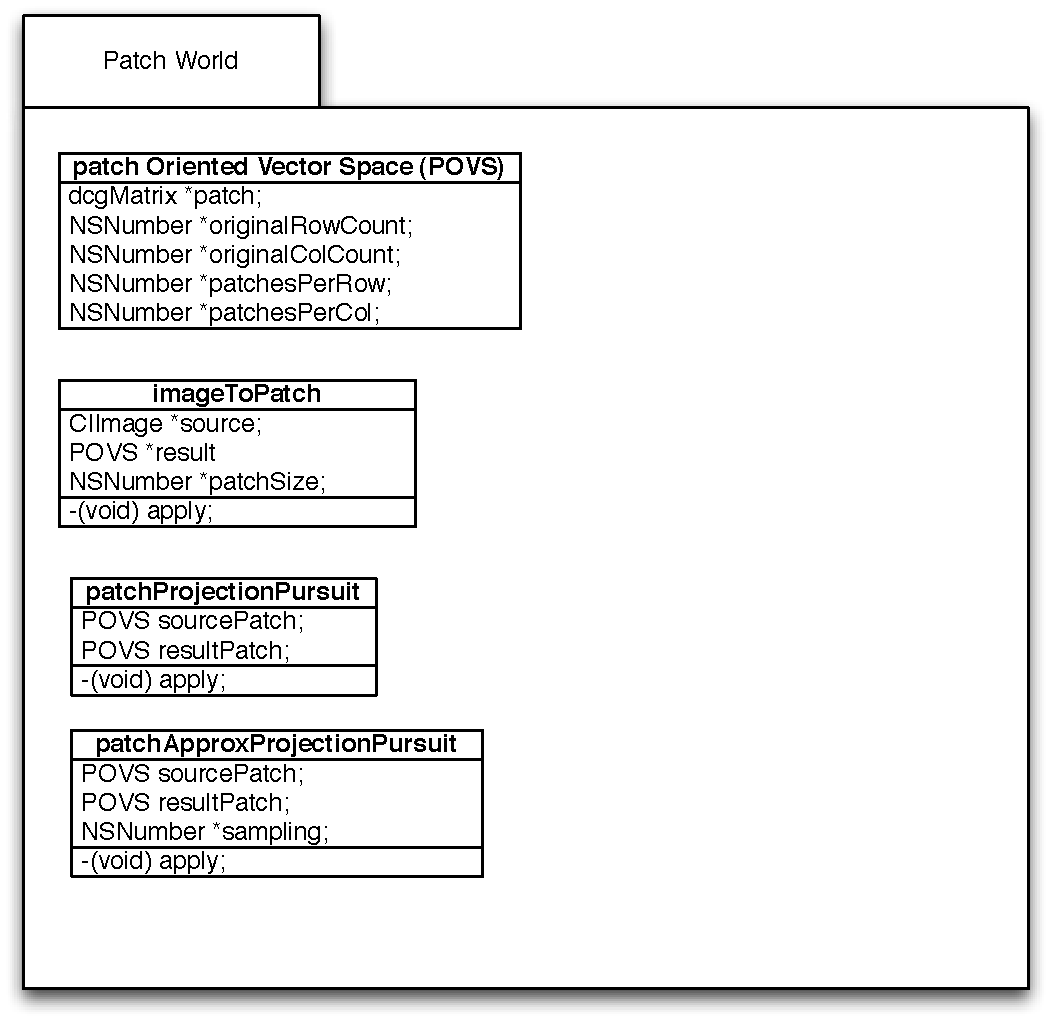
\includegraphics[width=4in]{patchWorld.pdf} 
%   \caption{Patch World Framework}
%   \label{fig-patch-world}
%\end{figure}


\subsection{Connection between Independent Component Analysis and Sparse Code Shrinkage}
\label{ica-scs-connection}

The constraints on Sparse Code Shrinkage are included in the following list.  Accompanying these requirements are comments that show the connection of Sparse Code Shrinkage to ICA. 
\begin{enumerate}
\item First, using a noise-free training set of $\vec{x}$, use some sparse coding method for determining the orthogonal matrix $\mathbf{W}$ so that the components $s_i$ in $\vec{s} = \mathbf{W}\vec{x}$ and so that $\vec{s}$ has as sparse a distribution as possible.  Estimate a density model $p_i (s_i)$ for each sparse component. 
\begin{itemize}
	\item Note that if $\vec{x}$ is already whitened, then the ICA mixing matrix is a transformation matrix satisfying the constraints on $\mathbf{W}$.
	\item The exponential and Laplace density functions are specific components to the non-polynomial projection pursuit family. 
\end{itemize}


\item Invert the relation $\vec{s} = \mathbf{W}\vec{x}$  to obtain estimates of the noise-free $\mathbf{x}$, given by $\mathbf{\hat{x}}(t) = \mathbf{W}^T \hat{\mathbf{s}}(t)$.
\end{enumerate}
The matrices $\mathbf{W}$ and $\mathbf{A}$ are mixing matrices.  Under the constraint that both  $\vec{s}$ and $\vec{x}$ are zero mean and unit variant, then $\mathbf{W}= \mathbf{A}^{-1} = \mathbf{A}^T$.


\section{Mathematica implementation of Multiple Discriminant \\Analysis}
\label{mathematica-prototype-mda}
The Mathematica version is a straight-forward implementation and possess a copy of the data set supplied via a worksheet.  %is long and mostly comes from listing the samples directly in a worksheet.  
%Other than that, the steps mimic the algorithm for MDA very closely.  %Once the 
The structure allows for a classifier to be constructed on the assumption that the data is Gaussian.  A listing of the Mathematica implementation to solve the Iris data-set is included in Appendix \ref{listing-mathematica-iris}.

% Double checked as of Nov 30
The variables setosa, viriginica, and versicolor  contain the original measurements.  Each observation is defined in a row matrix, and is named %We next construct a row matrix that contains data observations at each of its rows, called in the Mathematica code, 
barSetosaArray.  This array is used to generate $\vec{x_i} - \mu$ for row vector $\vec{x_i}$ in the setosa collection, which is misnnamed  normSetosa.  This allows the mean to construct the scatter matrix for setosa.  

The same thing was done for versicolor and virginica.  As stated in the preliminary sub-section on MDA (subsection \ref{mda-description-subsection}) %algorithm, 
$\mathbf{S_w}=  \sum_i S_i$ where $S_i$ are the scatter matrices for each of the classes.  The background set is obtained by %We also combine 
combining the flowers using the join method, %in Mathematica and take 
and obtaining the mean of the combined whole.  From there, %we use 
the mean array concept is used to reduce the action of finding the background scatter to matrix addition, scalar multiplication, matrix multiplication, and a transpose.  
Thus, mapping the original data source via the $\mathbf{W}$ obtained is simply a matter of matrix multiplication.  The results of equation \ref{mathematica_system} are shown in Figure \ref{mathematicaPlotsUsingManualMDA}.

This  implementation demonstrates some characteristics inherent to MDA that make its implementation for practical production image processing systems.  First and for most is the need to identify each member of the classification prediction set.  These elements construct the scatter matrices for each classification.  For classical data analysis, this is practical as observations are supplied as collection of measurements.  Therefore each measurement set can be collected into a vector, and each vector used to construct the scatter matrix pertaining to its classification.  In image analysis, scatter matrices imply that portions of the image comprise a similar observation vector.   One such concept is presented in the patch world section, but any arrangement of the elements of an observed image may be used to perform such a set of analyses.  Another characteristic, defined in equation \ref{mathematica_system} where $S_B$ is the background scatter matrix, is that the combined points belonging to the classifications and points not belonging to them at all comprise the background data-set used to construct the background scatter matrix, as is the case in PCA.  This second characteristic is the easier to accommodate, generally.  What happens the background is selected at random, and the within scatter matrix is selected notably fewer from known points?   How do these data-sets get selected.   It is one thing to gather the points and encode them into a MDA algorithm.   For a practical system it does require a sufficient interface so that users need not rewrite the system just to use it.   

% Proofed as up to this point as of Nov 2, 2007

%Fortunately, Mathematica has an intuitive method for computing eigenvectors of a generalized system like the following:% below.
\begin{equation}
\mathbf{S_w} \vec{e_i} = \lambda_i \mathbf{S_B} \vec{e_i} \label{mathematica_system}
\end{equation}


%\subsection{Plot Results from Mathematica}
\begin{figure}[htbp] %  figure placement: here, top, bottom, or page
   \centering
   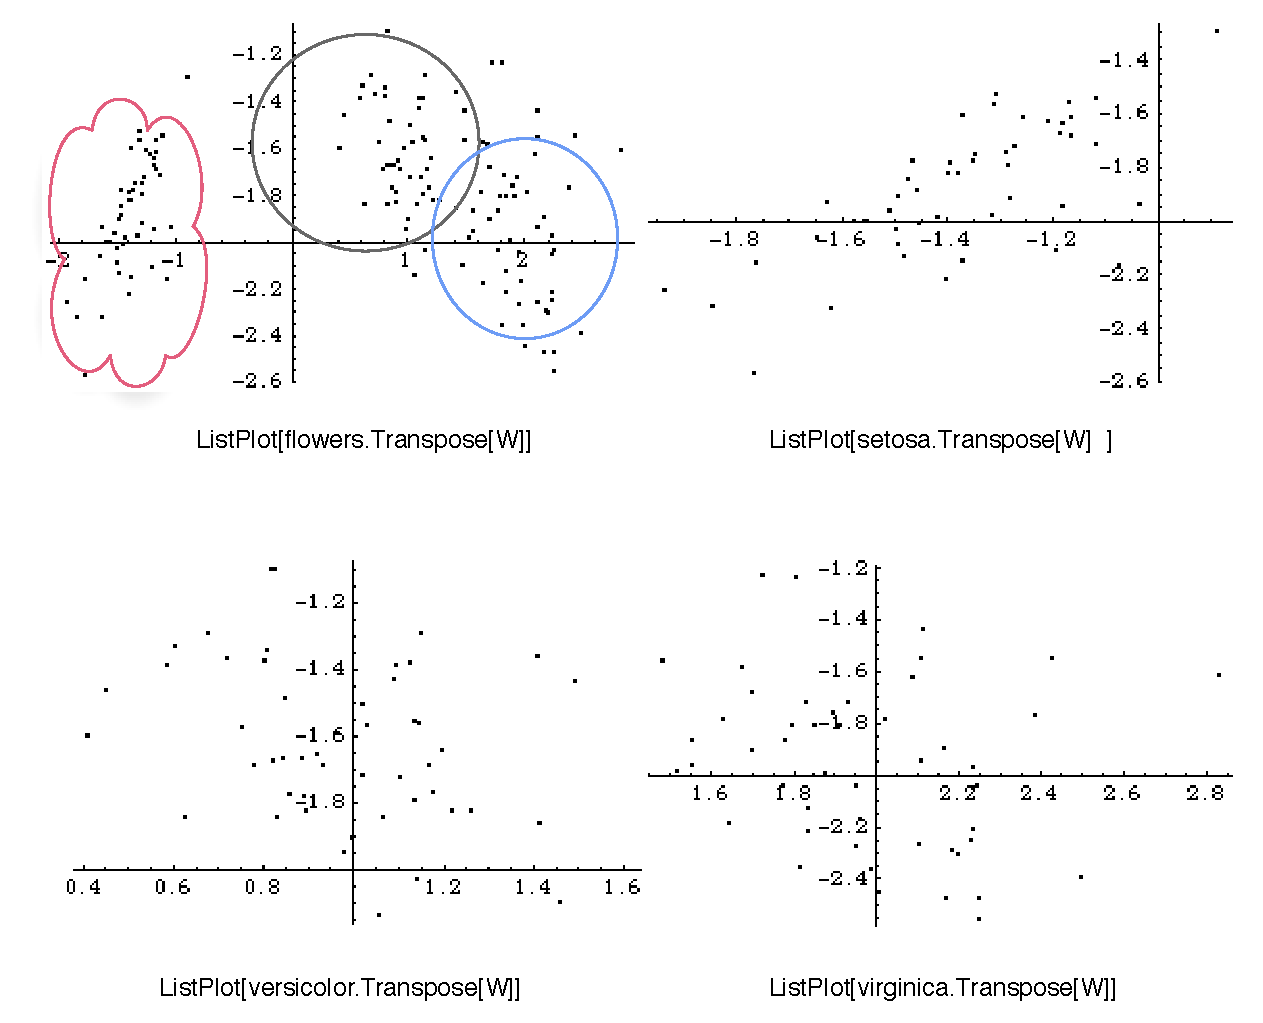
\includegraphics[width=5in]{flowersMDA.pdf} 
   \caption{Mathematica Plots using a manual MDA}
   \label{mathematicaPlotsUsingManualMDA}
\end{figure}

\section{Evolution of CPU Bound Solutions}
\subsection{Octave and Core Graphics Implementation of Expected Maximization}\label{classic-em-implementation}
The first experiment conducted for this paper implements a product using Octave (an open source product similar to Matlab). %implementation for convenience.    
In this example, there is an original image of a human optic disc.  From this image, %was used to observe 
a histogram of normal distribution functions is computed to assist in determining a model, shown in equation \ref{sum-of-probabilities}.  %The model assumes  that the data are the sum of these distributions.   
%One of the first experiments tried on the EM segmentation experiment was conducted in Octave (Matlab's Open Source cousin).   In this example, I fed in the original optic disc image along with the request for 5 classifications.   
The results are seen in Figures \ref{histogram-optic-disc} and \ref{histograms-optic-disc}.  %One of the things noticed 
Significant in this implementation of the EM segmentation is the use of histograms as opposed to the generation of a structure with normal distribution structure for the sample data. 
\begin{equation}
p(x | \vec{\theta}) = \sum_i p_i(x | \vec{\theta}_i) \label{sum-of-probabilities}
\end{equation}

  


\begin{figure}[htbp] %  figure placement: here, top, bottom, or page
   \centering
   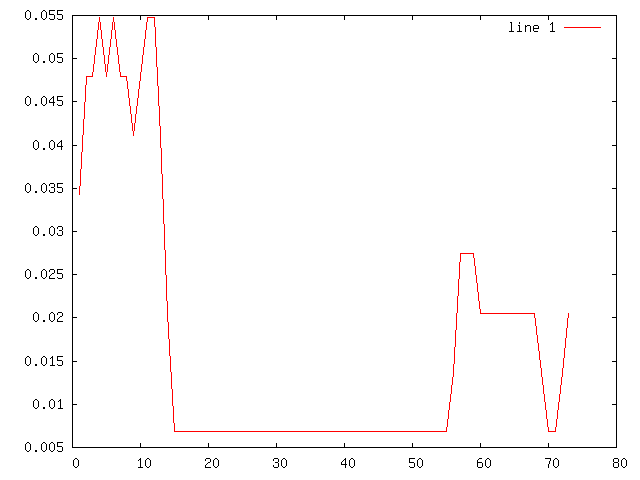
\includegraphics[width=3in]{plot.png} 
   \caption{This figure is a plot of Guassian sums for the optic disc.}
   \label{histogram-optic-disc}
\end{figure}


\begin{figure}[htbp] %  figure placement: here, top, bottom, or page
   \centering
   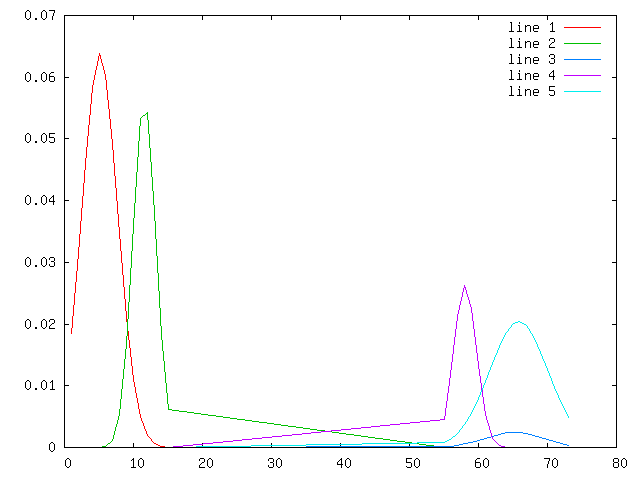
\includegraphics[width=3in]{probability.png} 
   \caption{This is a plot of sub-Gaussian components for the optic disc.}
   \label{histograms-optic-disc}
\end{figure}

The Octave prototype supplied some insight that led to the designing of an Objective-C version. 
During the development of the Objective-C with Core Graphics, unit tests were used to verify each component developed.   Each of these tests used a small data set.  Once the data set became large, rapid allocation and deallocation becomes a constraint on performance.   
%However, most unit tests do not require a document window to allow the results of each unit to be selected and examined individually or in a combined fashion.  

% Proofed up to this point, Nov 5 11:00 am

\subsubsection{Core Graphics Version}
All of the EM implementations generate a set of statistical classes defined by a set of sufficient statistics.  Each collection provides a method of classifying every subsequent element. % in to one of these classifications.  
In the case of image processing, these classifications represent a collection of masks.  These masks identify segments to either be retained or eliminated.  

A consequence of this need is that the interface consists of an additional panel.  %One of these panels contains a table or listing of each component of the sample image.  The other references the controller's array of masks.  The checking of a box in the masks panel applies the mask to the original image, and adds it to the result.  The removing of the check of a mask, subtracts that application of the mask.  
The panel contains a slider to control the number of normal distributions constructing the estimate of the image.  The original design is shown in Figure \ref{emComponentSelection}. In the final model demonstrated in figure \ref{segmentsPanel}, a table inside the panel shows a selection of specific distributions and displays them by mean and variance.  At the time this report was written, only one distribution could be selected at a time.  The reason for the limitation was to allow the mask to be produced and rendered in reasonable time.   Selecting a component causes a mask to to be constructed for the univariate component %selected
chosen.  Changing the number of distributions causes the distributions estimations to be computed via EM.


\begin{figure}[htbp] %  figure placement: here, top, bottom, or page
   \centering
   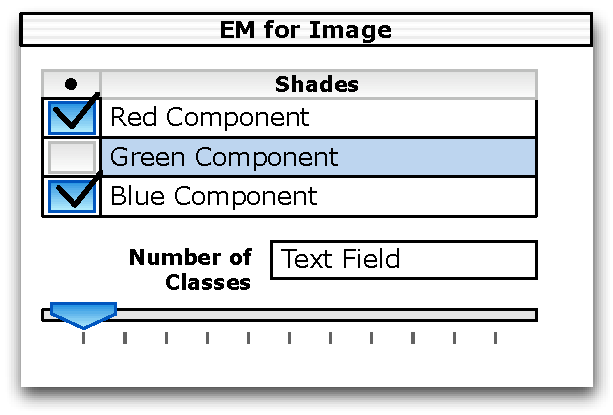
\includegraphics[width=3in]{emComponentSelection.pdf} 
   \caption{The results of an ``EM for Image'' are
a set of segmenting classifiers and the 
masks that result from the classification}
   \label{emComponentSelection}
\end{figure}


\begin{figure}[htbp] %  figure placement: here, top, bottom, or page
   \centering
   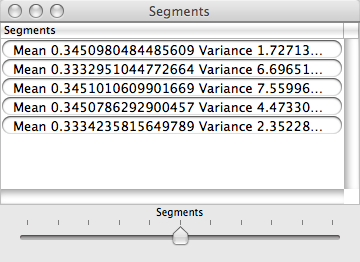
\includegraphics[width=3in]{segmentsPanel.png} 
   \caption{EM Segments shown by mean and variance for a photo of a human iris.}
   \label{segmentsPanel}
\end{figure}

A mask has the sole purpose of blending sections of the image.   In this case, either the color point belongs, or it does not.     It is in constructing these masks  that Core Graphics Data Providers and Image Providers become useful.   Also, %it is here where the 
in this construction DCGMatrix, obtained from the Grey-Scale Bitmap, is reused and fed into the classifier.  If the point belongs, a white value is inserted into the mask.  The mask is black otherwise.   Note that a true color filter would use a multivariate variety of the classifier, as it is a vector (color vector).  Using this technique, the need to construct a new form of the image itself is eliminated as the mask can be fed into a Core Image filter with the original image for display and rendering.   

\subsubsection{First Successful GUI Model}
The first successful version used a subclass of NSOpenGLView and model controller to test the concept of an EM filter.  A better version should move the computation to a CIFilter and use threads to move the computation away from the main display thread.   Otherwise, the intensity of the computation can overwhelm the main thread and waste the existence of multiple-core CPUs and computational grids.   With the first version, the controller includes a panel to show the segments (displayed by mean and variance shown in Figure \ref{segmentsPanel} ) and view window that shows the image masked with the selected segment.  If no segment is selected, the mask is clear and shows the original image, as shown in Figure \ref{fiveEmSegments}.  
There is the possibility of computing the EM directly from the Graphics Card, but that implies providing an expected step kernel, a maximization step kernel, and a termination test kernel.

It is this hybrid Core Image - Core Graphics approach introduced in earlier versions of this report that offers the ability use classic CPU oriented computation with GPU oriented filters.  Core Image is itself a GPU bound computation mechanism for computing powerful filters, with a skeleton running CPU bound to provide control.  Mask blending is a rudimentary GPU bound practice, and does not need to be computed CPU bound.  This technique does save time, enough to make the difference between a responsive GUI based application and an unresponsive one.  Another approach that is even more efficient is to use the mean and variance parameters as control methods to a Core Image filter designed specifically for such classifications.  This causes the CPU bound computation to be limited to computing the summed normal model itself.  But that implementation is scheduled for another report. 

%Selecting a component causes a mask to to be constructed for the univariate component selected.  %The removing of such a selection must inherently remove the selection from its associated masks, as they would be destroyed in the process.  
%Also, one other design decision solely for the purpose of the experiment the number of classes are determined by a slider control.  %As such, this number is applied to all sub-components.  A design depiction of this panel is shown in figure.
\subsubsection{Design Details and Considerations}
The two steps for EM are explicitly stated in listing \ref{lst_computeEM} .  %One consequence of this development show revelations about necessary steps for its computation.    
The estimation step is computed implicitly% first 
before the loop and again at the end of the loop.  The reason for computing the estimation step is to determine the estimation termination value.    Another issue of implementation, revealed in listing \ref{lst_maximizationStepEM}, %shows 
is the need for careful zeroing of summing values.  The previous mean is needed in computing the maximization steps variance.    Therefore, careful application of order ensures maximum efficiency, for CPU bound computations, of both expectation and maximization steps.  %caution must be applied as to when the mean is computed.  


%In even the simplicity of 
The univariate case has the possibility that the EM algorithm will require many iterations.  %A consequence is the results from each iterative step.
One design decision is whether to retain the results of each iteration of the EM algorithm.  In some cases, these steps may be discarded.  Others they must be retained.  In this implementation,  the results of the maximization and estimation steps are recycled in each subsequent iteration.  The presumption is that the sufficient statistics computed in both the last and next to last maximization step have in fact converged.  Convergence of the result is measured by the values of the estimation function computed in each estimation step.  While it is a waste to compute the maximization upon convergence, it is also harmless.  %Thus the initialization of the univariate object is defined in listing \ref{lst_initializeEM}.


% Proofed upto Nov 6 11am
Another presumption needed in any implementation of the EM algorithm is initial values.  %In this case, 
These initial values are produced upon initializing the EM object.  The object containing the EM algorithm is initialized with the samples to build the estimator and the number of distributions in the summation equation.  In listing \ref{lst_initializeEM}, mean, variance, and proportions are each of the class dcgVector, which is an Objective-C wrapper around a C-array with helper methods typical for vector operations.  The mixture member is a dcgMatrix, which is a wrapper around a C two dimensional array with methods suitable for matrix operations.  
Other components are needed in the Objective-C version to make it more viable, and this is where design decisions must be considered.   In the initial design, obtaining the image data itself was a matter of drawing to a Core Graphics Grey-Scale Bitmap and copying the data out.   This forces the computation to be CPU bound.  Either CPU bound or Graphics Processing Unit (GPU) bound versions are acceptable.   This subsection illustrates the CPU bound version.   A future report may review the GPU bound equivalent.  

In order to continue with a DCGMatrix obtained from a Core Graphics Grey-Scale Bitmap, it must be transformed into a vector of equal number of elements.  This vector and the number of desired classifications must then initialize an object to compute the EM Univariate Normal.    Once initialized, it is convenient to extract the results into an NSArray containing the sufficient statistics.  Such an array need not retain the proportions value.  

%Once obtain the array of sufficient statistics becomes the classifier for every grey scale value in the image.  In this case, the user is allowed to select which classifiers he/she wishes to see.   It is the point of selecting classifiers that a mask is drawn.   

It should be noted that obtaining the DCGMatrix from the Core Graphics Grey Scale Bitmap is quite tricky.  It is one section that is anything but universal between PowerPC (PPC) and Intel x86 architectures.   Care has to be taken to ensure byte ordering on the bitmap.  Otherwise, the results are garbage, and the EM will compute nonsense.  



\begin{figure}[htbp] %  figure placement: here, top, bottom, or page
   \centering
   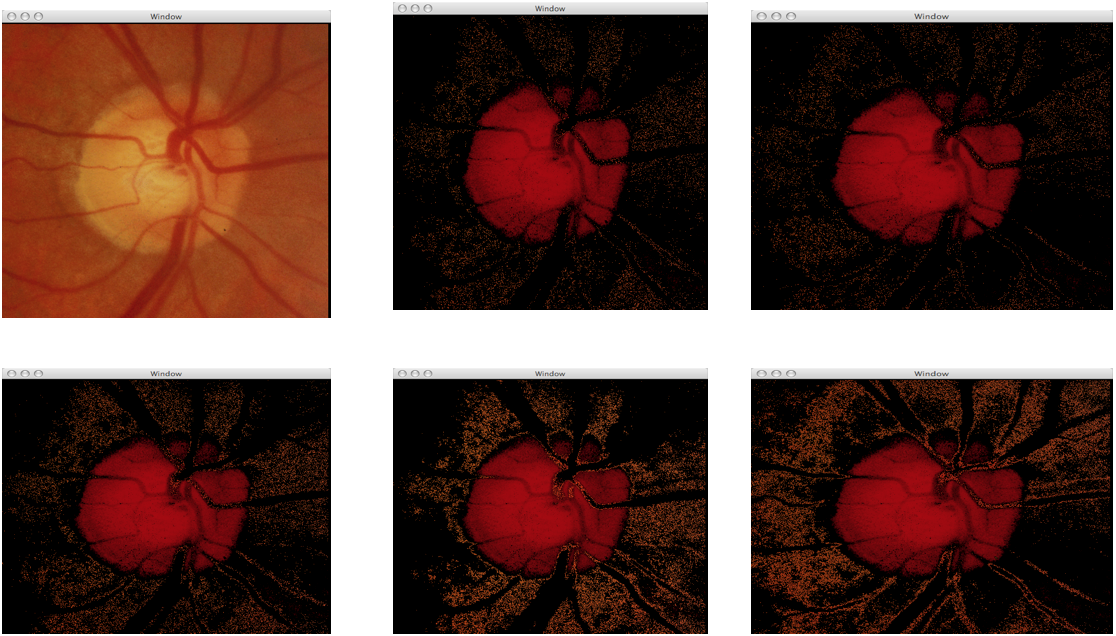
\includegraphics[width=6in]{fiveEmSegments.png} 
   \caption{Both the original image and 5 EM Segments of a human iris. }
   \label{fiveEmSegments}
\end{figure}

%Proof 27 Nov 2007
\subsection{Principal Component Anaylsis}\label{pca-classic-implementation}
%\subsection{The Early Steps}
%The first steps into building a PCA segment filter,  
In the first steps of constructing the PCA segment filter, two methods were considered, SVD and EVD, as many texts reference SVD as an efficient means of determining PCA.  %, what has been alluded to in many text as the most efficient CPU bound form of PCA, namely Singular Value Decomposition.  
%This version is readily
SVD is available in LAPACK and software packages that use it.  Building a filter for segmentation using SVD is another matter.   It is more intuitive to generate the mixing matrix for PCA, transform the data with it, filter the transformed data, and use the transpose of the mixing matrix to obtain the results.   Also, this straight-forward %from mathematical definition 
method of constructing PCA yields as byproducts the matrices needed to constitute a %is more intuitive when using PCA as a 
whitening agent to be used with Projection Pursuit.    

Also, using either EVD or SVD from LAPACK has debugging side-effects that tend to be difficult to trace.  Both decompositions implemented in LAPACK have an advantage in the fact they have optimized implementations such as the Accelerate framework (as called in OSX 10.3 to 10.5).  Thus, there is a trade-off between the ability to debug and determine which input to these functions was in error, versus speed of actual execution due to the vector pipeline acceleration.  

Observations made during the first set of tests of the EVD and SVD implementations using Quartz Composer plug-ins %test 
conducted for this report show the operations themselves to be efficient, but in order to be effective the multiplication elements have to use the C version of the Basic Linear Algebra Sub-routine (C-BLAS) implementation of matrix multiply (cblas\_dgemm in the Vector Library framework which is part of the Accelerate framework on OSX). In these cases the maximum size of the neighborhood still can not go above six by six pixels.  Without the  C-BLAS version of matrix multiplication the maximum pixel patch size is five by five.   The advantage of not using the C-BLAS version is that mistakes are easier to find and remove.  

Size of the data-set in tests conducted using Quartz-Composer as the facilitating tool have also been limited due to the time required to perform computations on the data.  If computation time exceeds certain limits, then the performance of the Quartz Composer editor becomes unstable and unusable.  Images in excess of 256 by 256 pixels are therefore scaled to a size within this limit.  %Also, the neighborhood size allowed  also must be limited in order to avoid the same stability issue.   
While stable, Quartz Composer is an excellent tool for observing how each component works in constructing principal components.  Such observations clarify subtle changes to the filter, which include  the number of neighborhoods, which eigenvectors to use during reconstruction, and the appearance of the principal components themselves.  All of these observations were intuitively available within a few mouse clicks.  


\subsubsection{Unit Test of PCA}
The experiment requested for this project is significantly more complex than what a unit test should test.  Any unit test should have a simple input, a simple output, and a known comparison for the output.   An example of this would be, say, a matrix shown in the following equation:  

\begin{eqnarray}
\mathbf{A}= 
\left\{
\begin{array}{llll}
1	& 	2 	& 	3	& 	4 \\
5	&	6	& 	7	& 	8 \\
9	&	10	&	11	&	12 \\
13	&	14	&	15	&	16 \\
\end{array}
\right\} \\
\mathbf{U} = 
\left\{
\begin{array}{llll}
-0.13		& 0.82	& -0.54	& 0.03 \\
-0.34 	& 0.42	&  0.75	& 0.36	\\
-0.54		& 0.03	& 0.13	& -0.8	\\
-0.75		& -0.36	& -0.341	& 0.42
\end{array}
\right\} \\
\mathbf{\Lambda}
\left\{
\begin{array}{llll}
38	& 0. 		& 0. 	&  0.\\
0.		& 2.07	& 0.	& 0.\\
0.		& 0.		& 0.	& 0.\\
0.		& 0.		& 0.	& 0.
\end{array}
\right\} \\
\mathbf{V}^T =
\left\{
\begin{array}{llll}
-0.42		& -0.71	& -0.16	& -0.52	\\
-0.47		& -0.27	& 0.60	& 0.57	\\
-0.52		& 0.17	& -0.72	& 0.41	\\
-0.56		& 0.61	& 0.28	& -0.47
\end{array}
\right\} \\
\textrm{SVD} (\mathbf{A}) = U \Lambda V^T \\
V = \textrm{eigenvectos}(\mathbf{A}\mathbf{A}^T) \\
\Lambda = \textrm{eigenvalues}(\mathbf{A}\mathbf{A}^T) 
\end{eqnarray}
The values for $\mathbf{U}$, $\mathbf{\Lambda}$, and $\mathbf{V}$ are computed using Mathematica's readily available SVD method.   A comparison between this and the unit test can be valuable. 
%Of course, Mathematica has pre-canned variety of the SVD, and we can simply use it to provide quickly a result can compare it to the results of the unit test.   

%Similarly, the results from the MDA assignment using Mathematica can be used as a unit test for the LDA/ MDA component.  The results are expected to be similar, within a scaling factor.  

\subsubsection{A Quartz Composer Model - CPU Bound}
There are methods to using Quartz Composer Plug-ins which allow them to rapidly prototype a PCA filter (or other filters of such consideration).  %It was originally 
The original %intended
intention was to use the Quartz Composer plug-in model to construct a GPU-bound solution to PCA, and that solution is still under consideration.   Even in a CPU-bound solution, Quartz Composer is useful for determining which handlers belong and how each feature contributes.  

As a multi-threaded environment, explicitly constructing new threads to explore and compute parts of a model is unnecessary as this is taken care of by the Quartz Composer development tool.   %Only detriment to this approach is that the complexity or size of computations must not become too large as this will cause instability.   
One detriment to this approach is that Quartz Composer requires each patch be responsive. A patch is a computational unit which is either a plug-in or system defined patch and consists of inputs, outputs, and specifications as to when to execute.   A few overhead plug-in patches were constructed for the handlers constituting the PCA model.   The composition, a collection of patches that constitute a graphical program, was constructed for this exercise as shown in Figure \ref{downsampled-pca-quartz-composer}.  The two images used to test this composition were the human iris image, used in the EM section (\ref{classic-em-implementation}), and a photo of Noe Lopez-Benitez from the Computer Science Department (Texas Tech University) web site.   Noe's photo was chosen for the size of the photo, which reduced the size of the samples and thus allowed unscaled tests of the composition.   %that would have and did fail for the larger human iris image when at full scale.  
Due to the size of the human iris photo, a scaling patch was inserted to maintain the 256 by 256 limit.

Another design consideration needed to comply with the instructions for the project was how the classifier worked on the principal components themselves.  The scatter matrix is defined in equations \ref{typical-scatter}.  This scatter matrix is determined by the mean matrix and correlation patches.  Covariance is a special case of correlation known as zero-mean correlation, and in this instance is convenient to keep in its more general form.  One improvement to be made to the method used in constructing the correlation patch could have been to use the  Basic Linear Algebra Subroutines (BLAS) implementation of matrix multiply to implement the patch (specifically the DGEMM included in the BLAS dense library).   With standard matrix multiplication, the patch does tend to consume excess computation time which takes away from the amount of computation that can be done responsively.  %If responsiveness is abused, then the Quartz Composer editor becomes unstable and tends to fail.  


%Proofed up to this point on Nov 27 .
The EVD patch has a handler object that computes the EVD via the LAPACK implementation.  The two outputs are the supplied matrix eigenvalues and eigenvectors.  Because the patch feeding the EVD patch is the correlation patch, the resulting eigenvectors are the mixing matrix for determining the principal components defined in equation \ref{principal-component}.  The subsequent patches are used to multiply the mixing matrix and the neighborhood samples to obtain the principal components.  At this point, any common data-oriented filtering technique may be applied.   In the first demonstration, a simple one-vector selection was applied.   This had an unintended result.   Figure \ref{downsampled-pca-quartz-composer} shows %The result was to take out 
sections of the image removed, which is consistent with the assumption that the component constitutes the classification.  % which may have belonged to some classification of the principal components.  
Such a technique causes the image to look as though it had been struck with a barrage of shotgun pellets.  

This method does provide insight into a GPU-bound version.  It is anticipated that size of the image will not be as much of a problem in a GPU-bound version as it is in the CPU equivalent.  Another useful insight gained by this implementation is that some of the filters, which would otherwise require many iterations of construction, can be defined.  A result of this insight is the possibility that a fixed size filter can be constructed once and used many times for this type of filtering in the GPU-bound version.


\begin{figure}[htbp] %  figure placement: here, top, bottom, or page
   \centering
   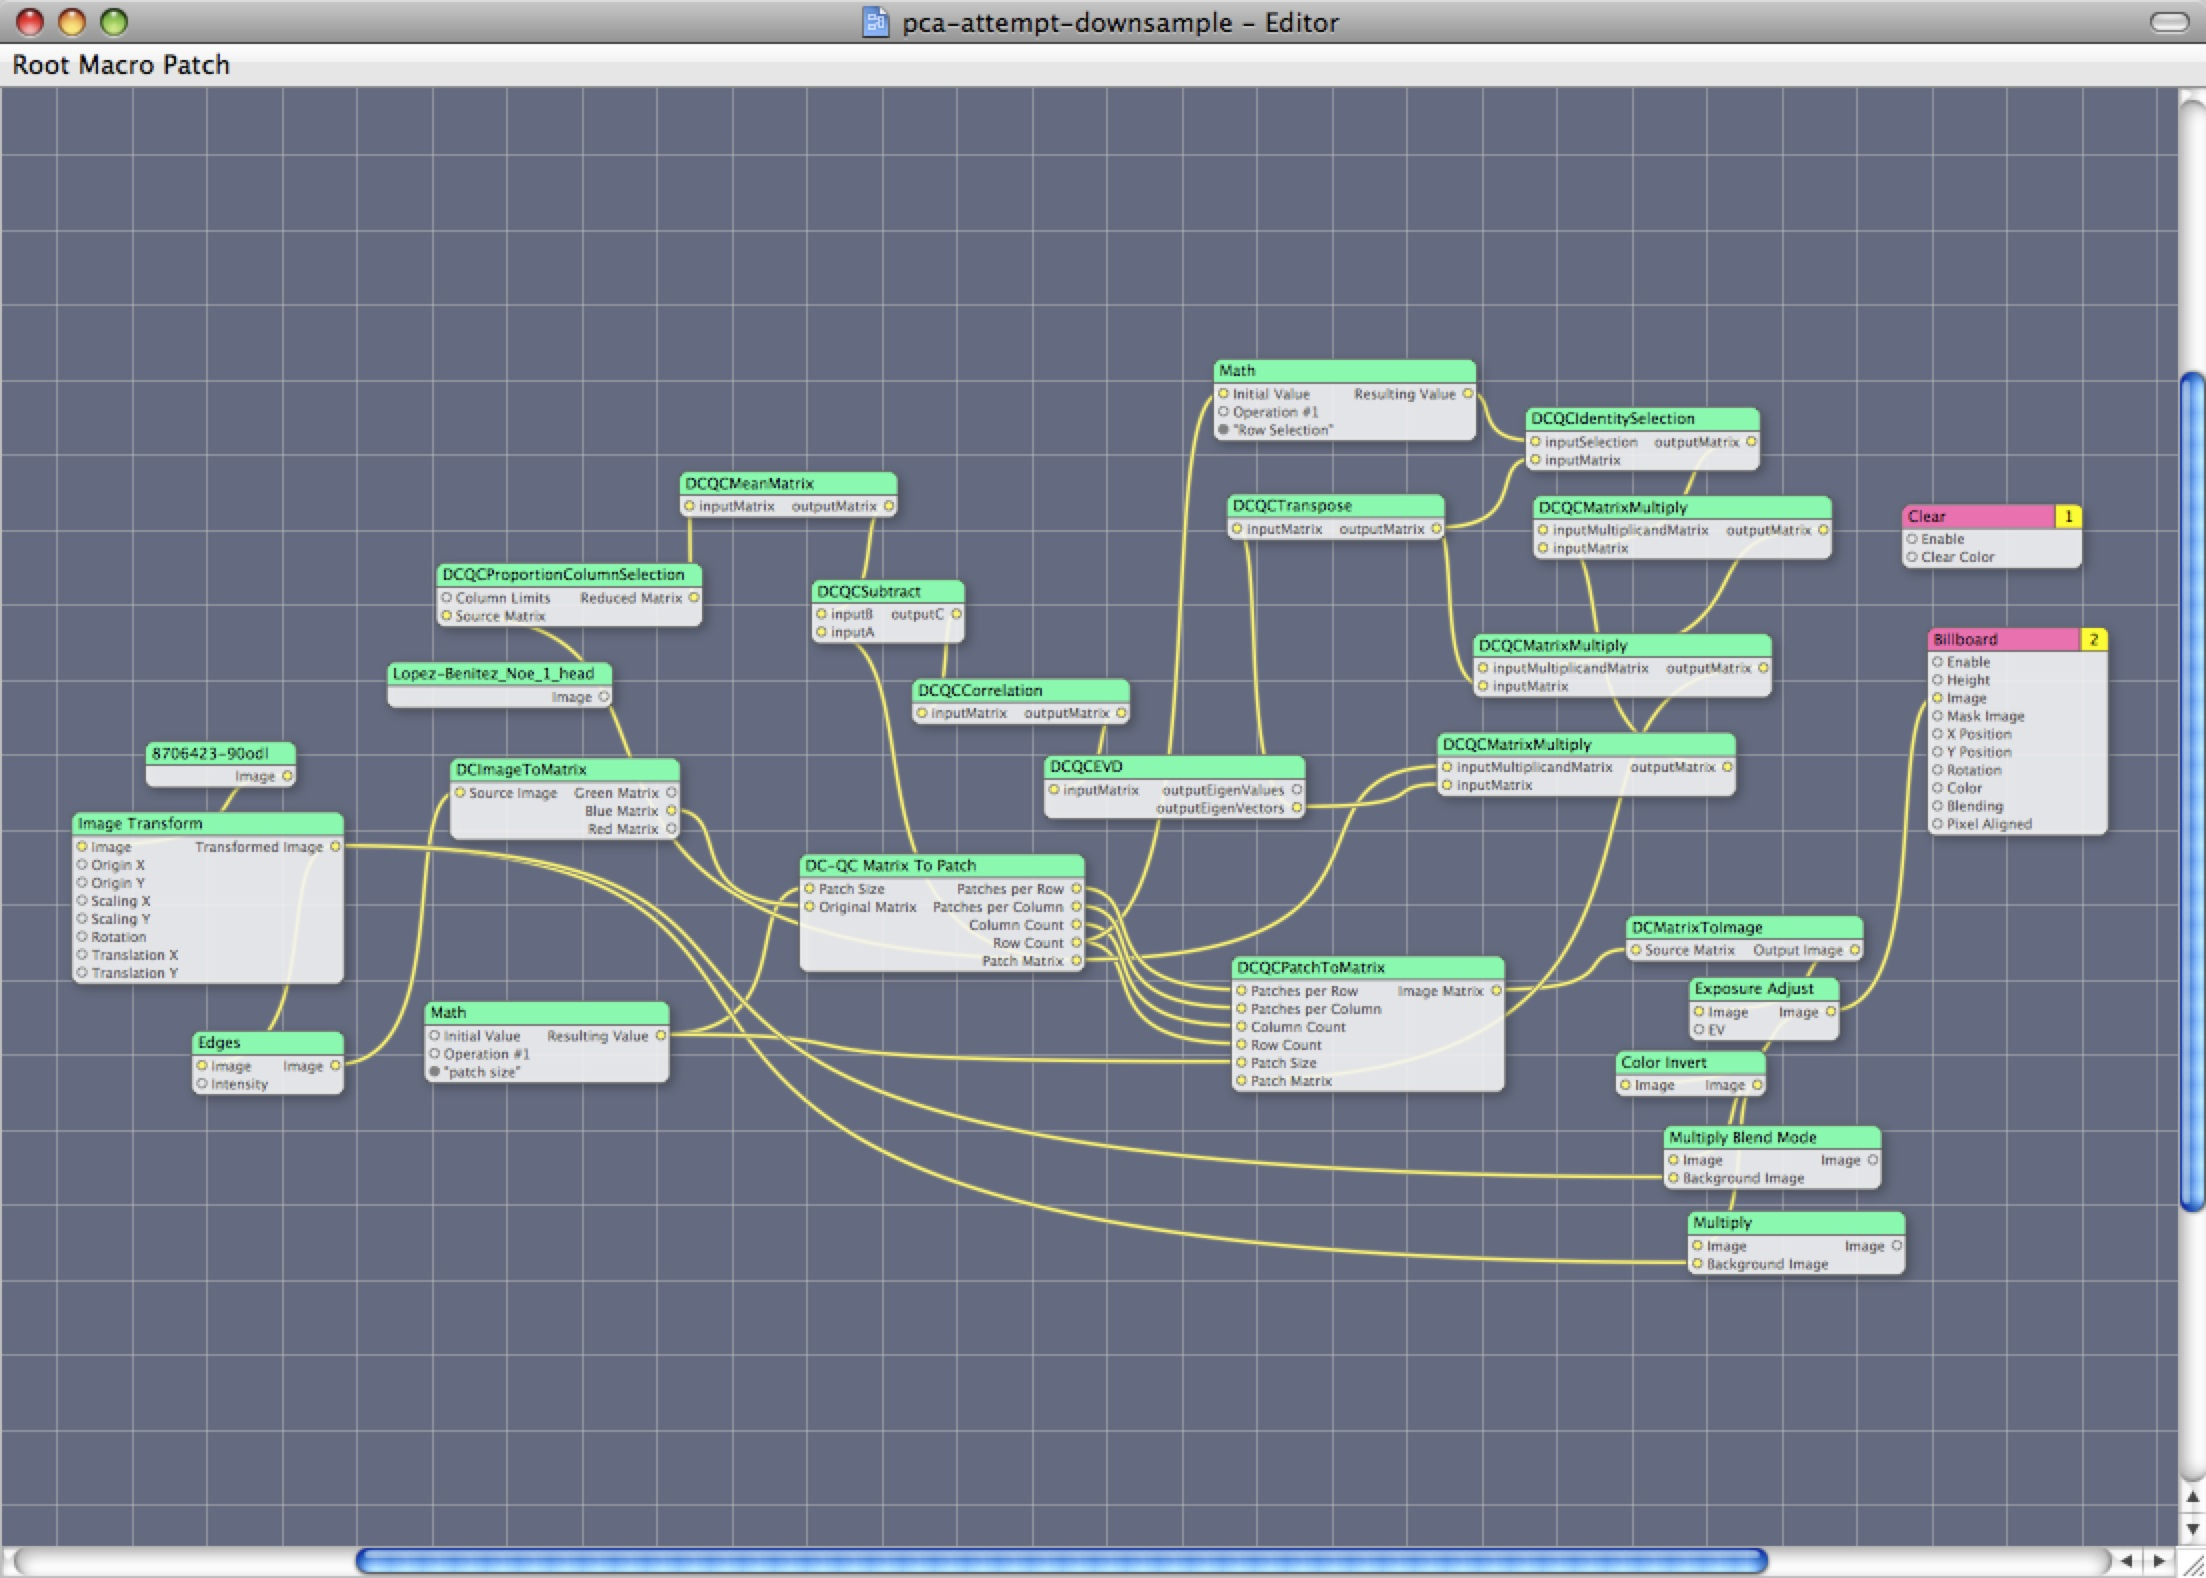
\includegraphics[width=3in]{pca-attempt-downsample.jpg} 
   \caption{A Quartz Composer patch for computing PCA via EVD.}
   \label{downsampled-pca-quartz-composer}
\end{figure}


\begin{figure}[htbp] %  figure placement: here, top, bottom, or page
   \centering
   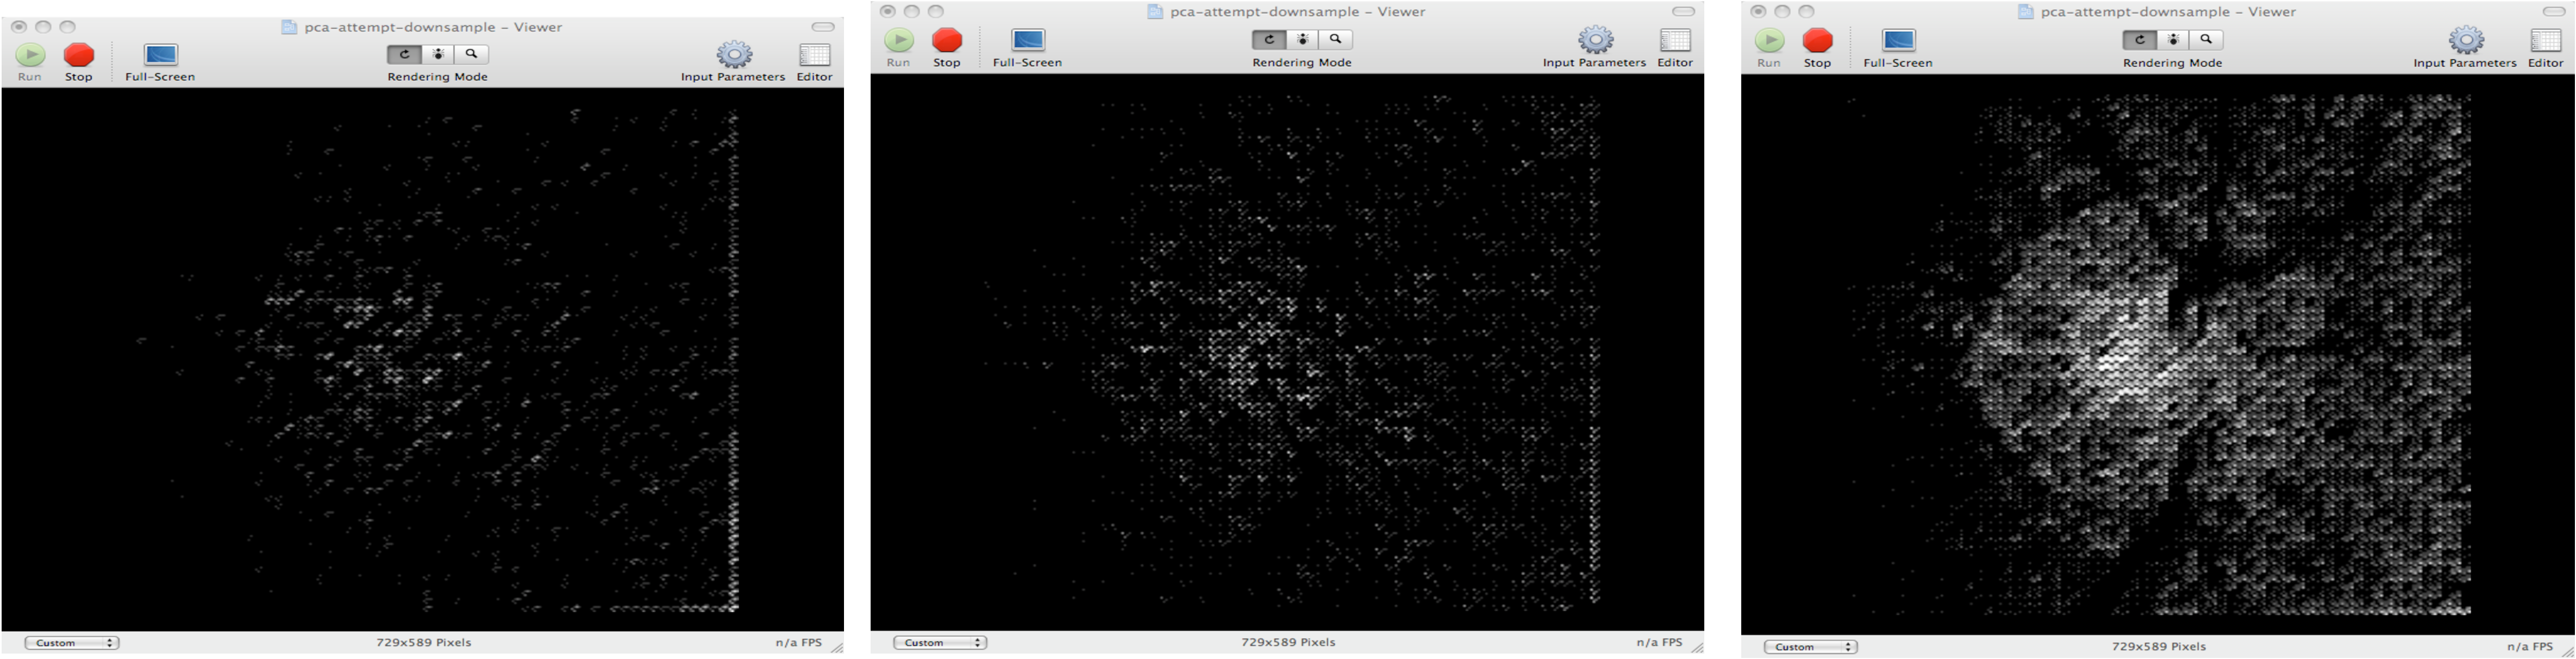
\includegraphics[width=5in]{lowerEyeRedChannel.pdf} 
   \caption{This is a set of results of a Quartz Composition PCA-Downsample of PCA via EVD.  In this sample, a few of the upper half principal components are shown.}
   \label{downsampled-pca-quartz-composer-lower-red-channel-eye}
\end{figure}


\begin{figure}[htbp] %  figure placement: here, top, bottom, or page
   \centering
   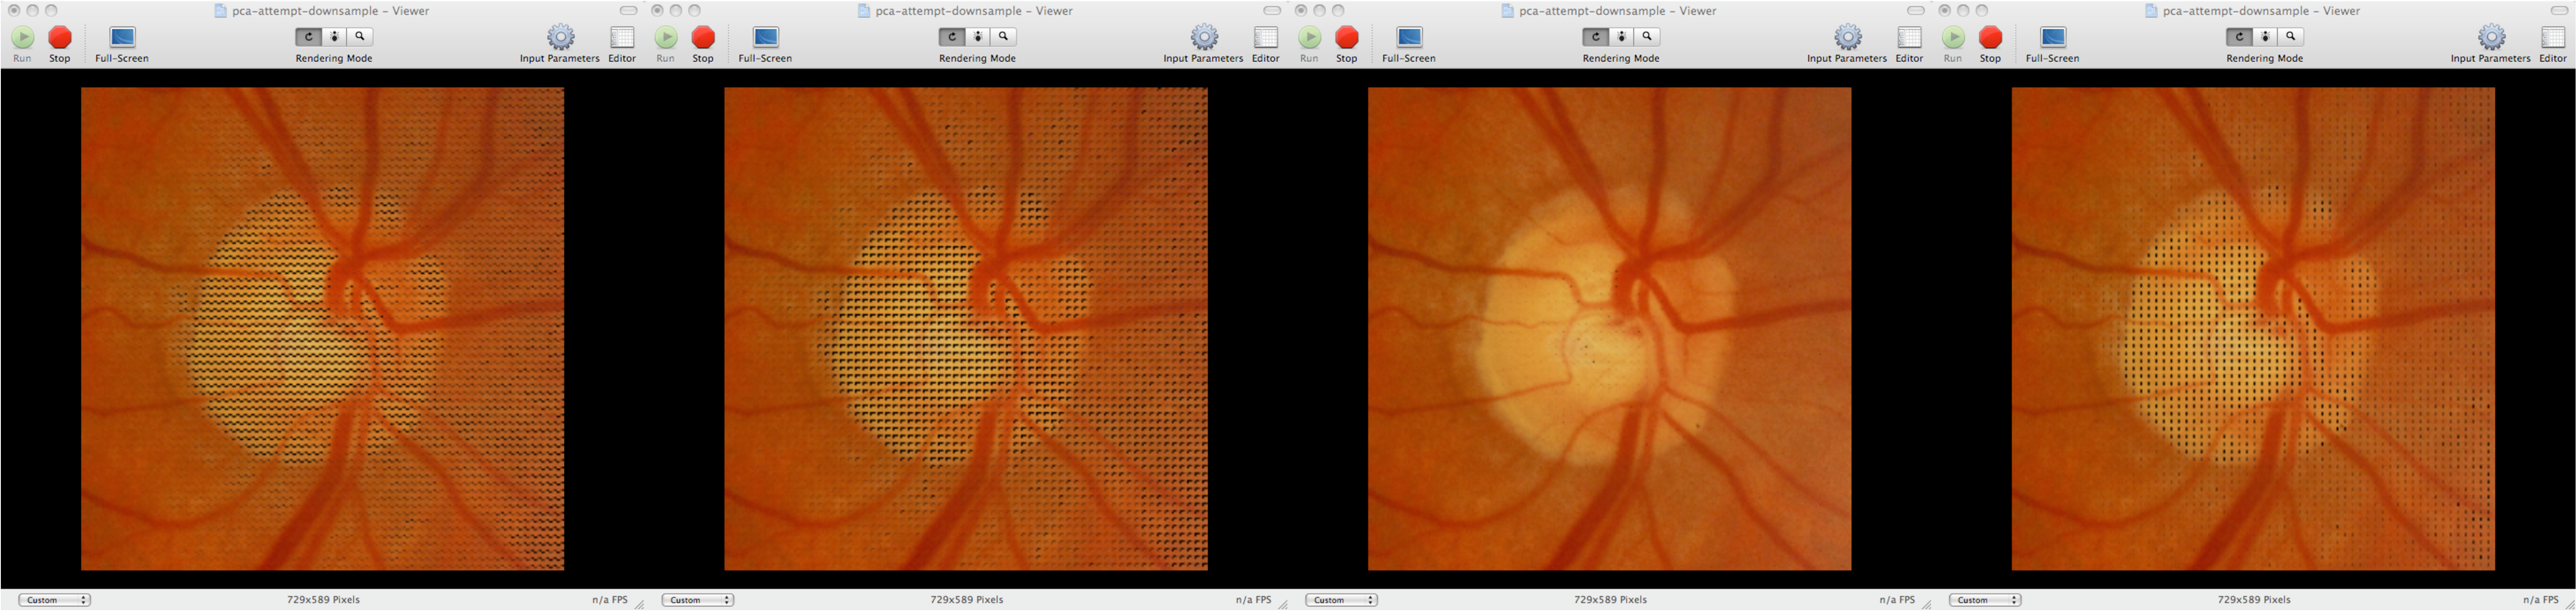
\includegraphics[width=5in]{eye-lower-green-channel-blended.pdf} 
   \caption{This is a set of results of a Quartz Composition PCA-Downsample of PCA via EVD.  In this sample, the green channel is used to provide the filter, and an enhancement is made on the filter elements themselves. }
   \label{downsampled-pca-quartz-composer-green-channel-blended}
\end{figure}


\begin{figure}[htbp] %  figure placement: here, top, bottom, or page
   \centering
   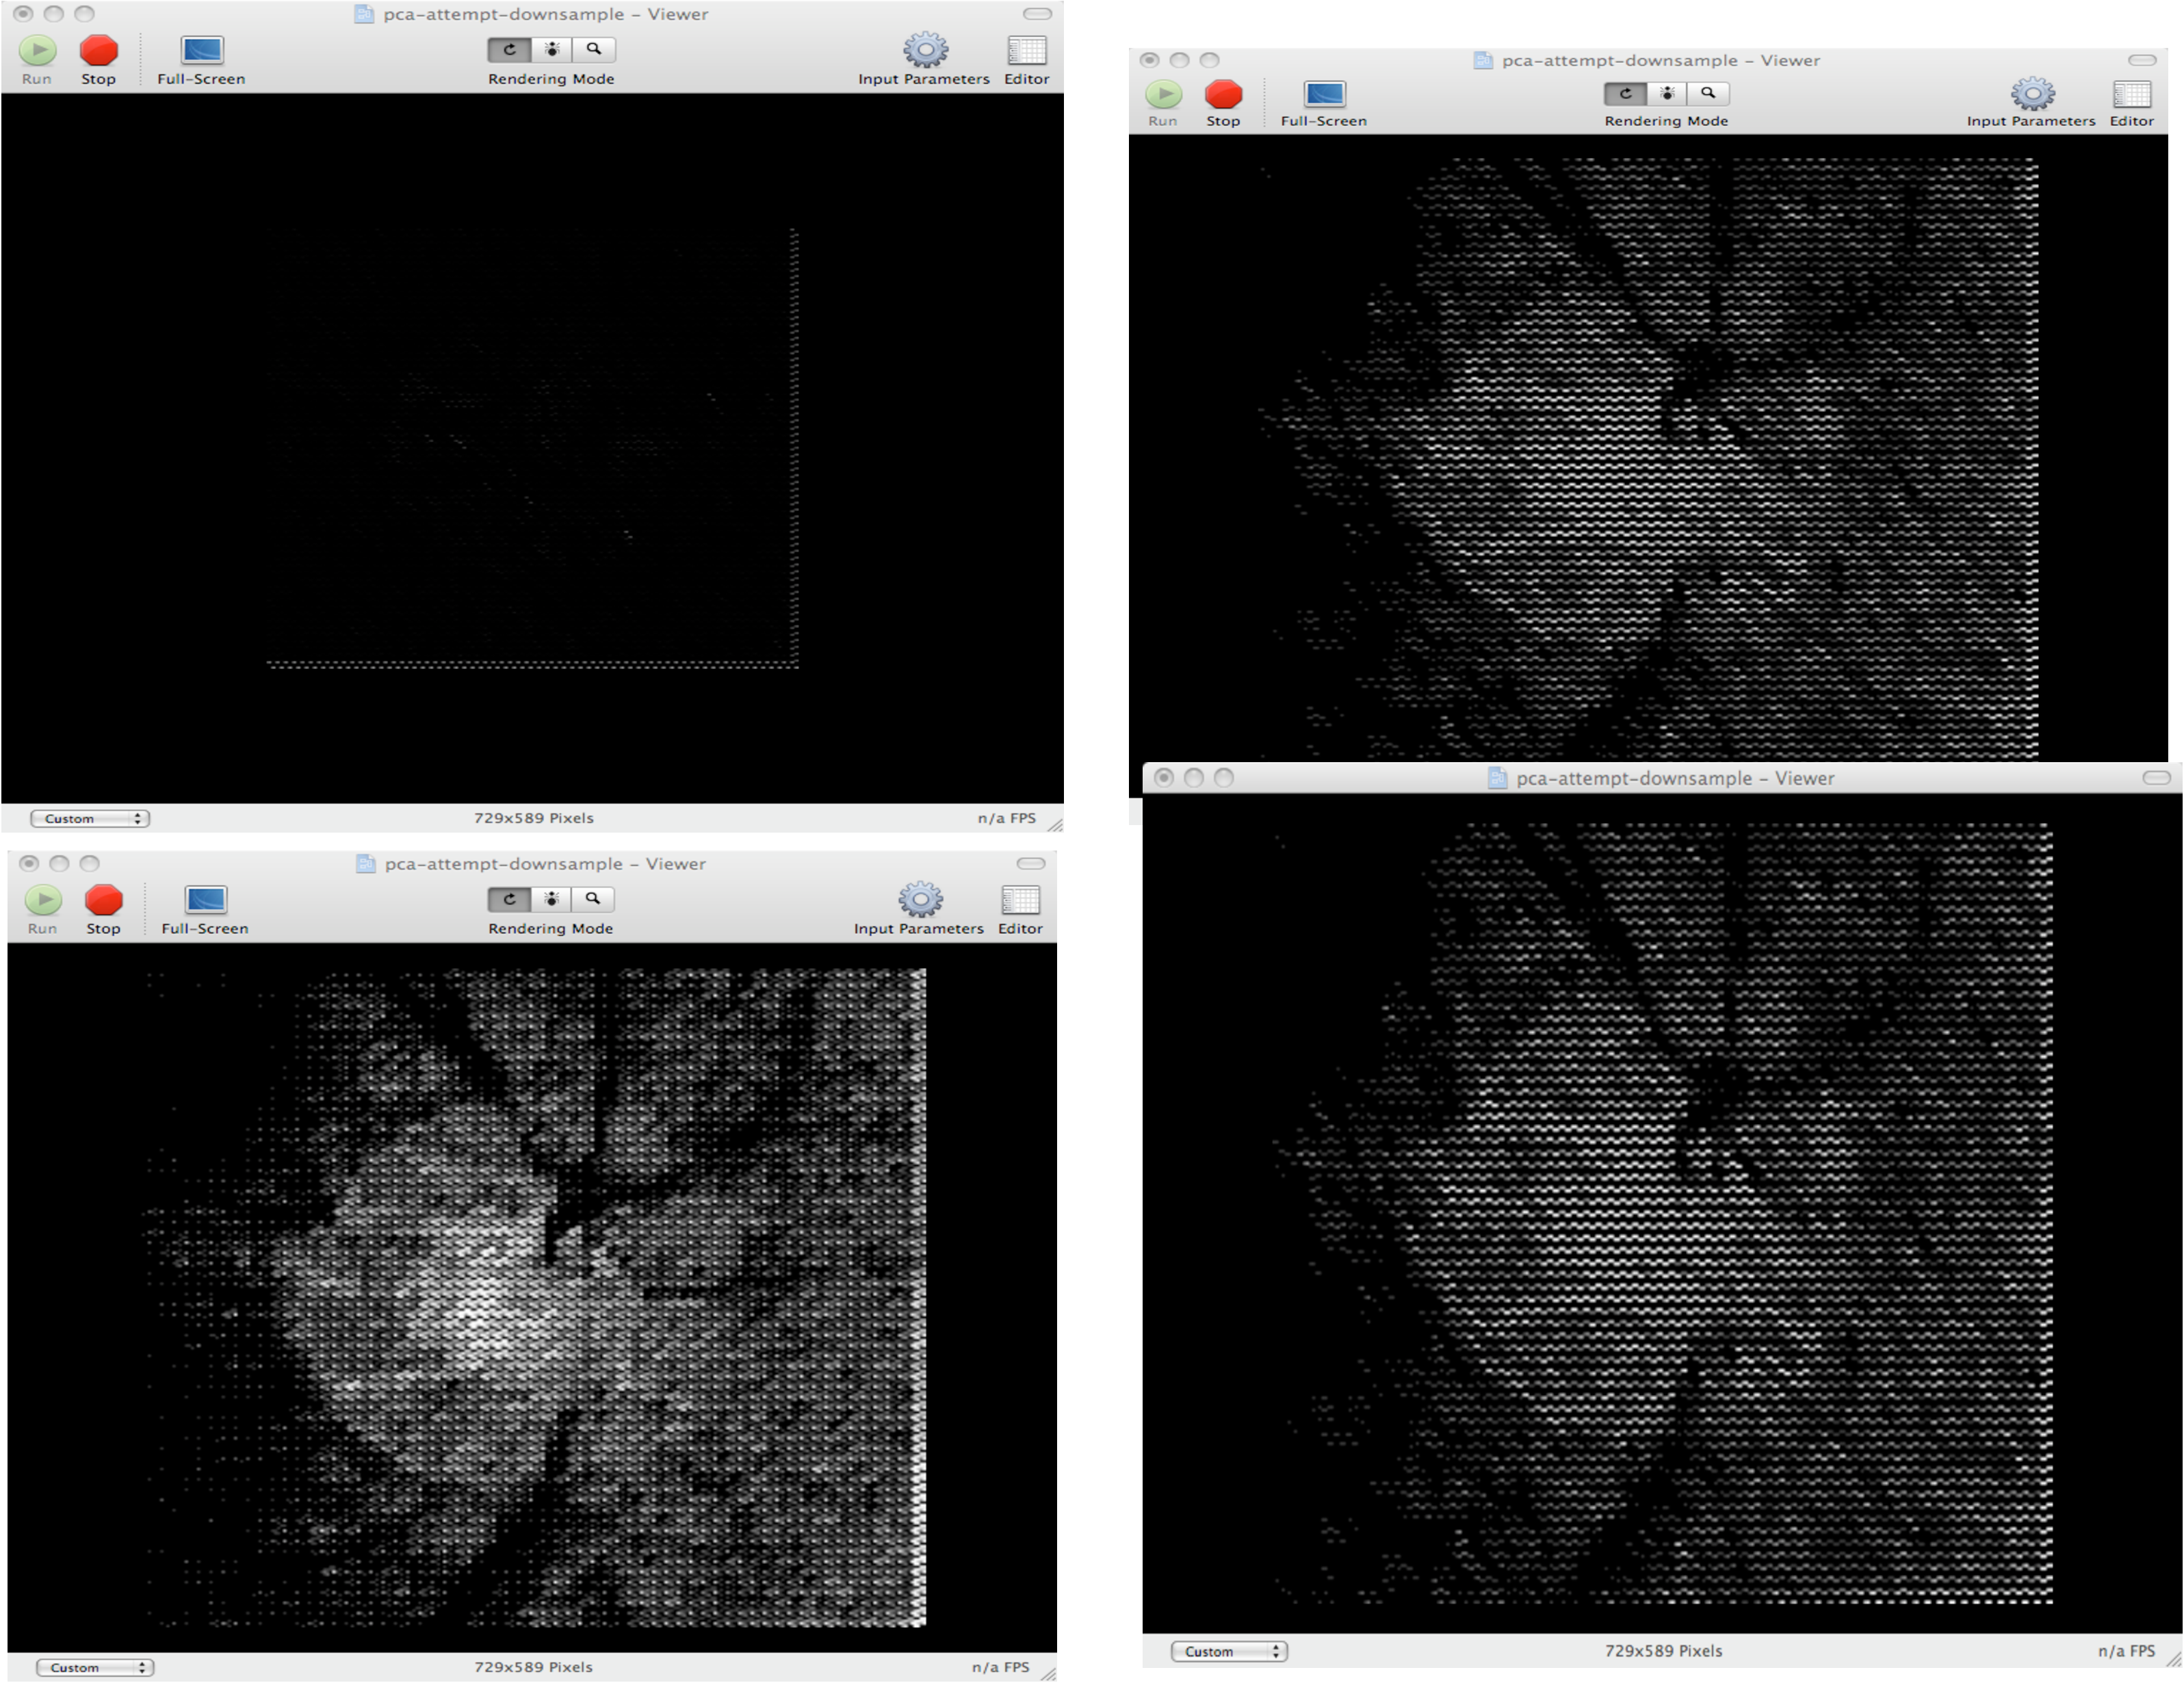
\includegraphics[width=5in]{red-channel-upper16.pdf} 
   \caption{This is a set of results of a Quartz Composition PCA-Downsample of PCA via EVD.  In this sample, the red channel is used with an enhancement.  These elements come from the lower principal components. }
   \label{downsampled-pca-quartz-composer-green-channel-blended}
\end{figure}

\subsection{Filters using ICA and PCA}\label{transformation-masking-maps}
Adapting a PCA filter to become an ICA filter is specified in the Algorithm \ref{alg:patch-oriented-sparse-coding-shrinkage-with-source}.  All of the steps of obtaining the neighborhoods and ensuring the data are whitened, or relatively whitened, are part of the mathematical definition of PCA.  Therefore, a projection pursuit patch can be inserted after the principal component stage.  Further, as stated, the transpose of the PCA mixing matrix is included with the ICA mixing matrix to obey the following equation:
\begin{equation}
\mathbf{X} = \mathbf{PAS} + \mathbf{M}
\end{equation}
where $P$ is the PCA mixing matrix and $\mathbf{A} = \mathbf{W}^T$ is the ICA mixing matrix.   Because projection pursuit is used in this case to determine the Sparse Coding Shrinkage, the size of $\mathbf{W}$ is $l^2 \times 1$, where $l$ is the size of the observation neighborhood vector.
\begin{figure}[htbp] %  figure placement: here, top, bottom, or page
   \centering
   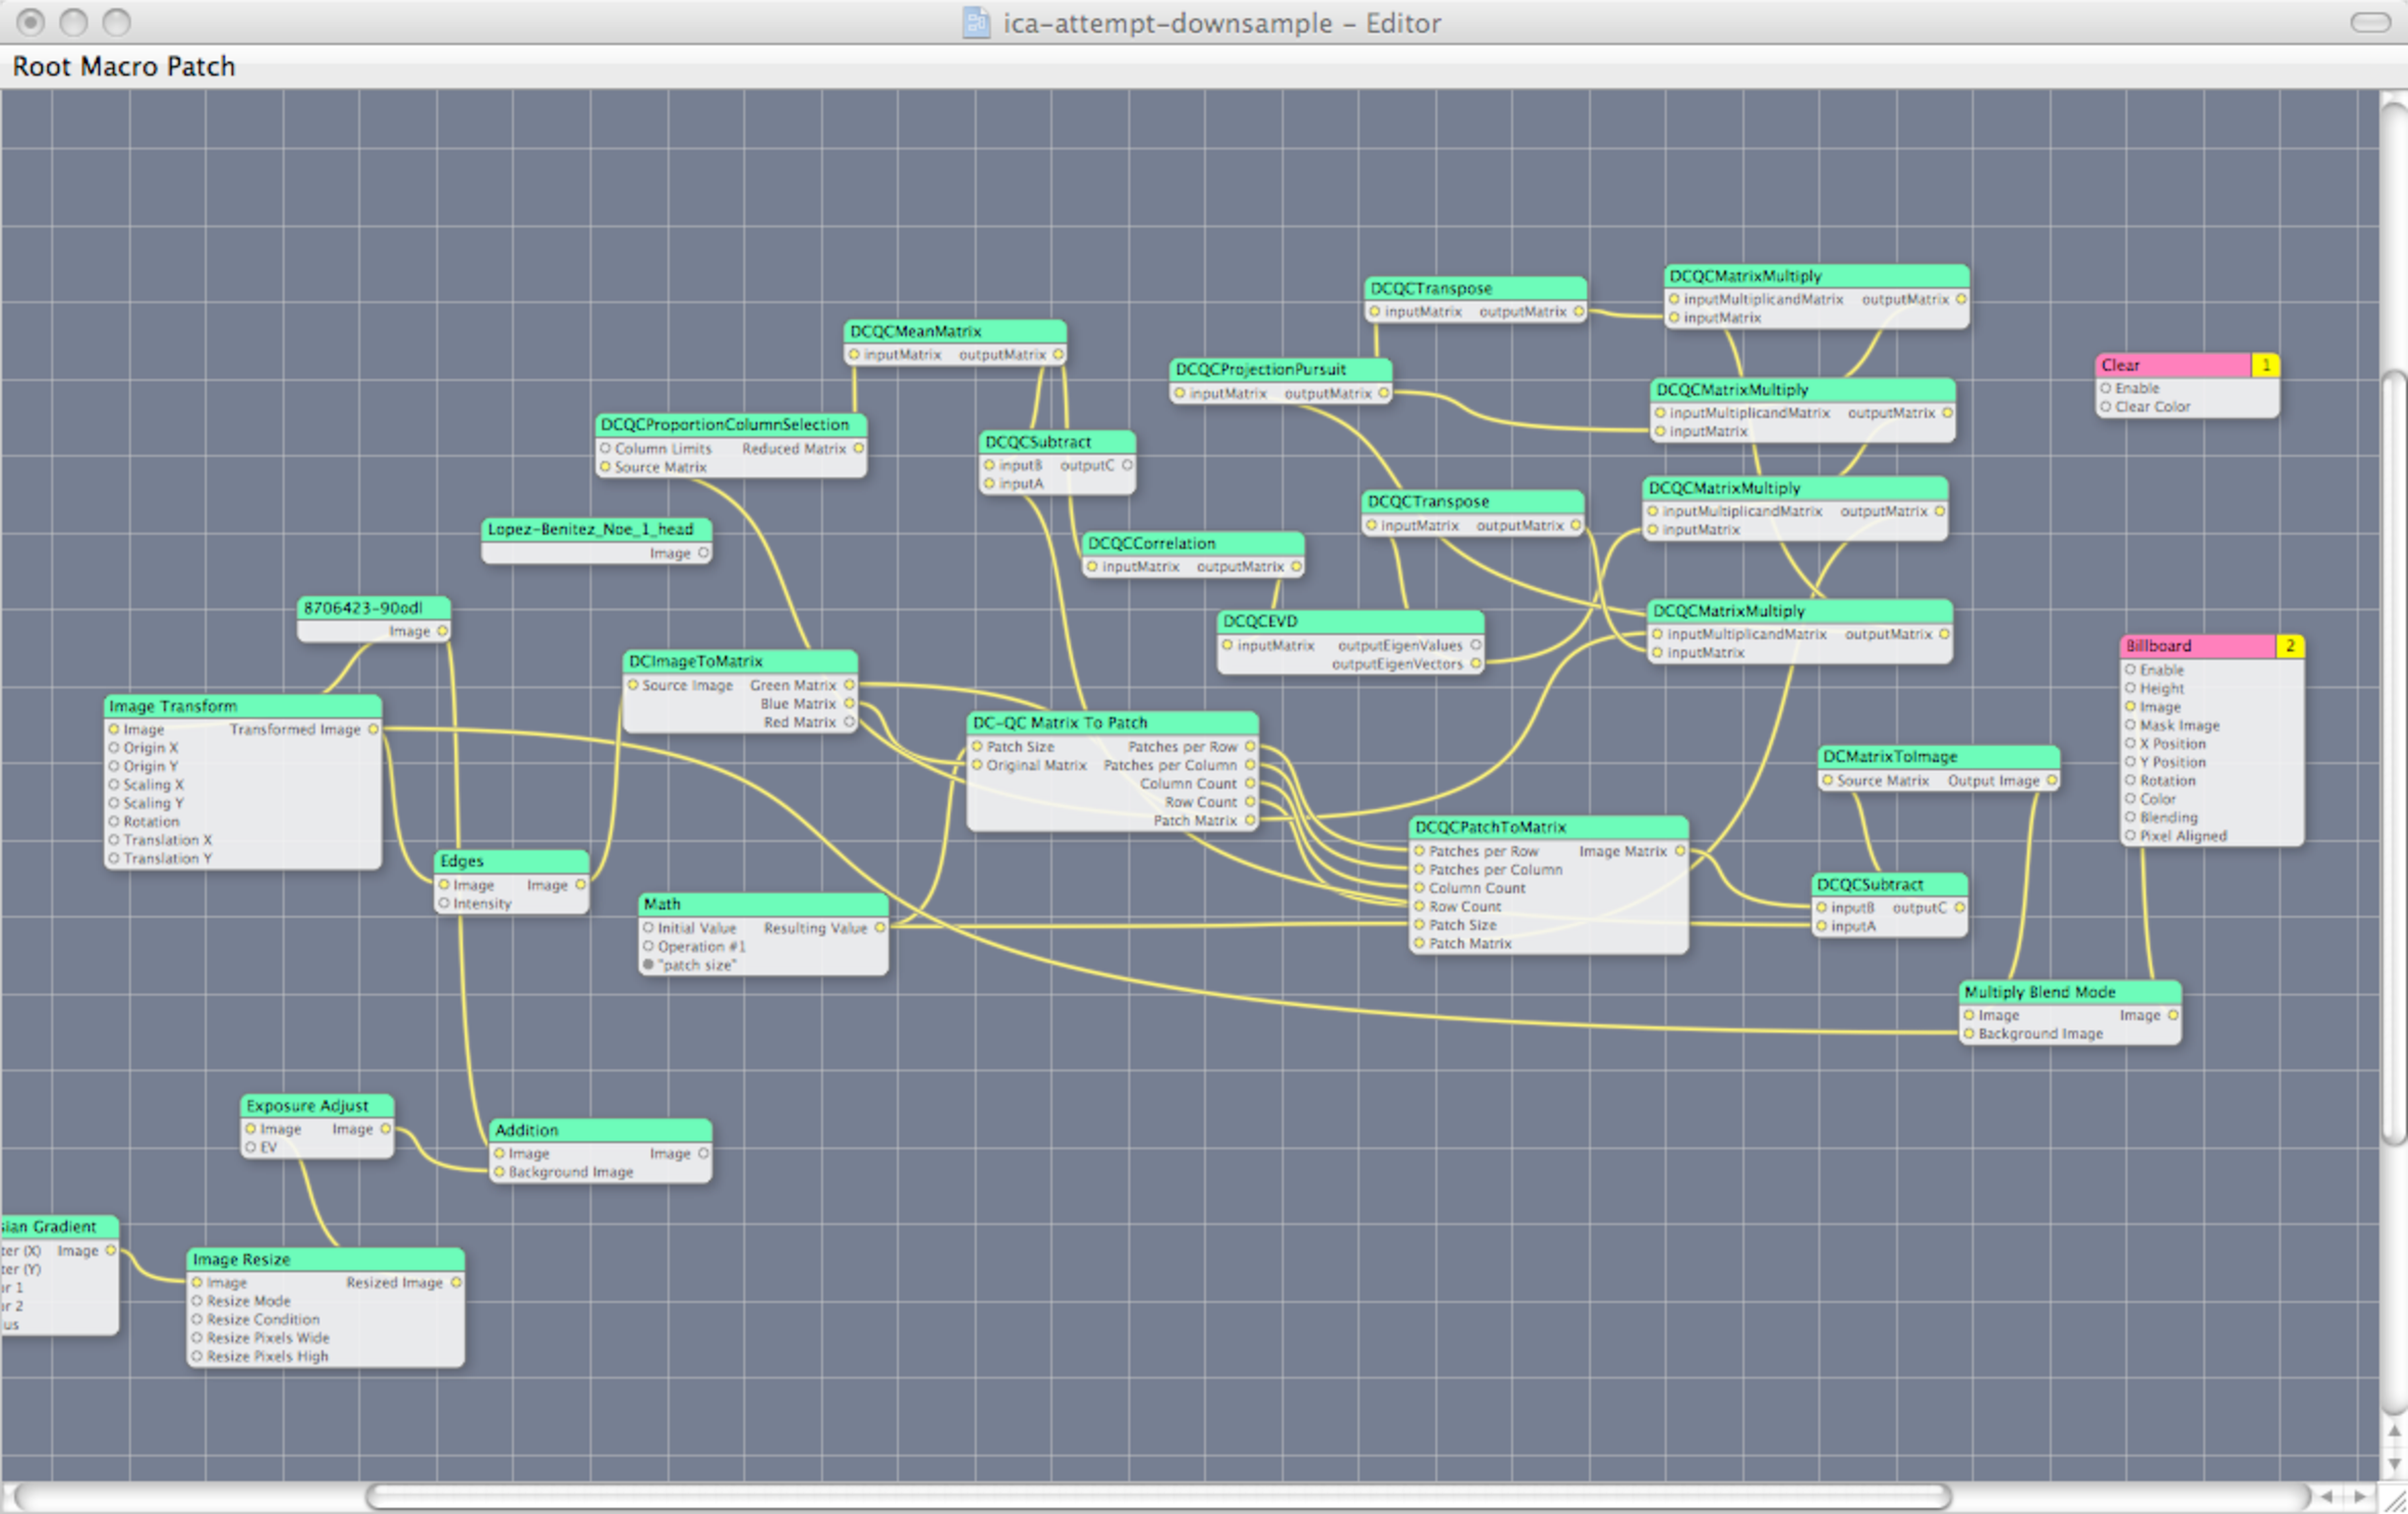
\includegraphics[width=6in]{ica-downsample.pdf} 
   \caption{A Quartz Composer patch for computing PCA via EVD.}
   \label{downsampled-pca-quartz-composer}
\end{figure}
One observation from applying the ICA filter to the human iris%, %the ICA filter
is that it has the effect of sharpening certain pixels within each neighborhood.   A neighborhood size of 2 by 2 tends to have the fewest side-effects from excessive information.   The 4 by 4 neighborhood size shows signs of excessive information loss.

\begin{figure}[htbp] %  figure placement: here, top, bottom, or page
   \centering
   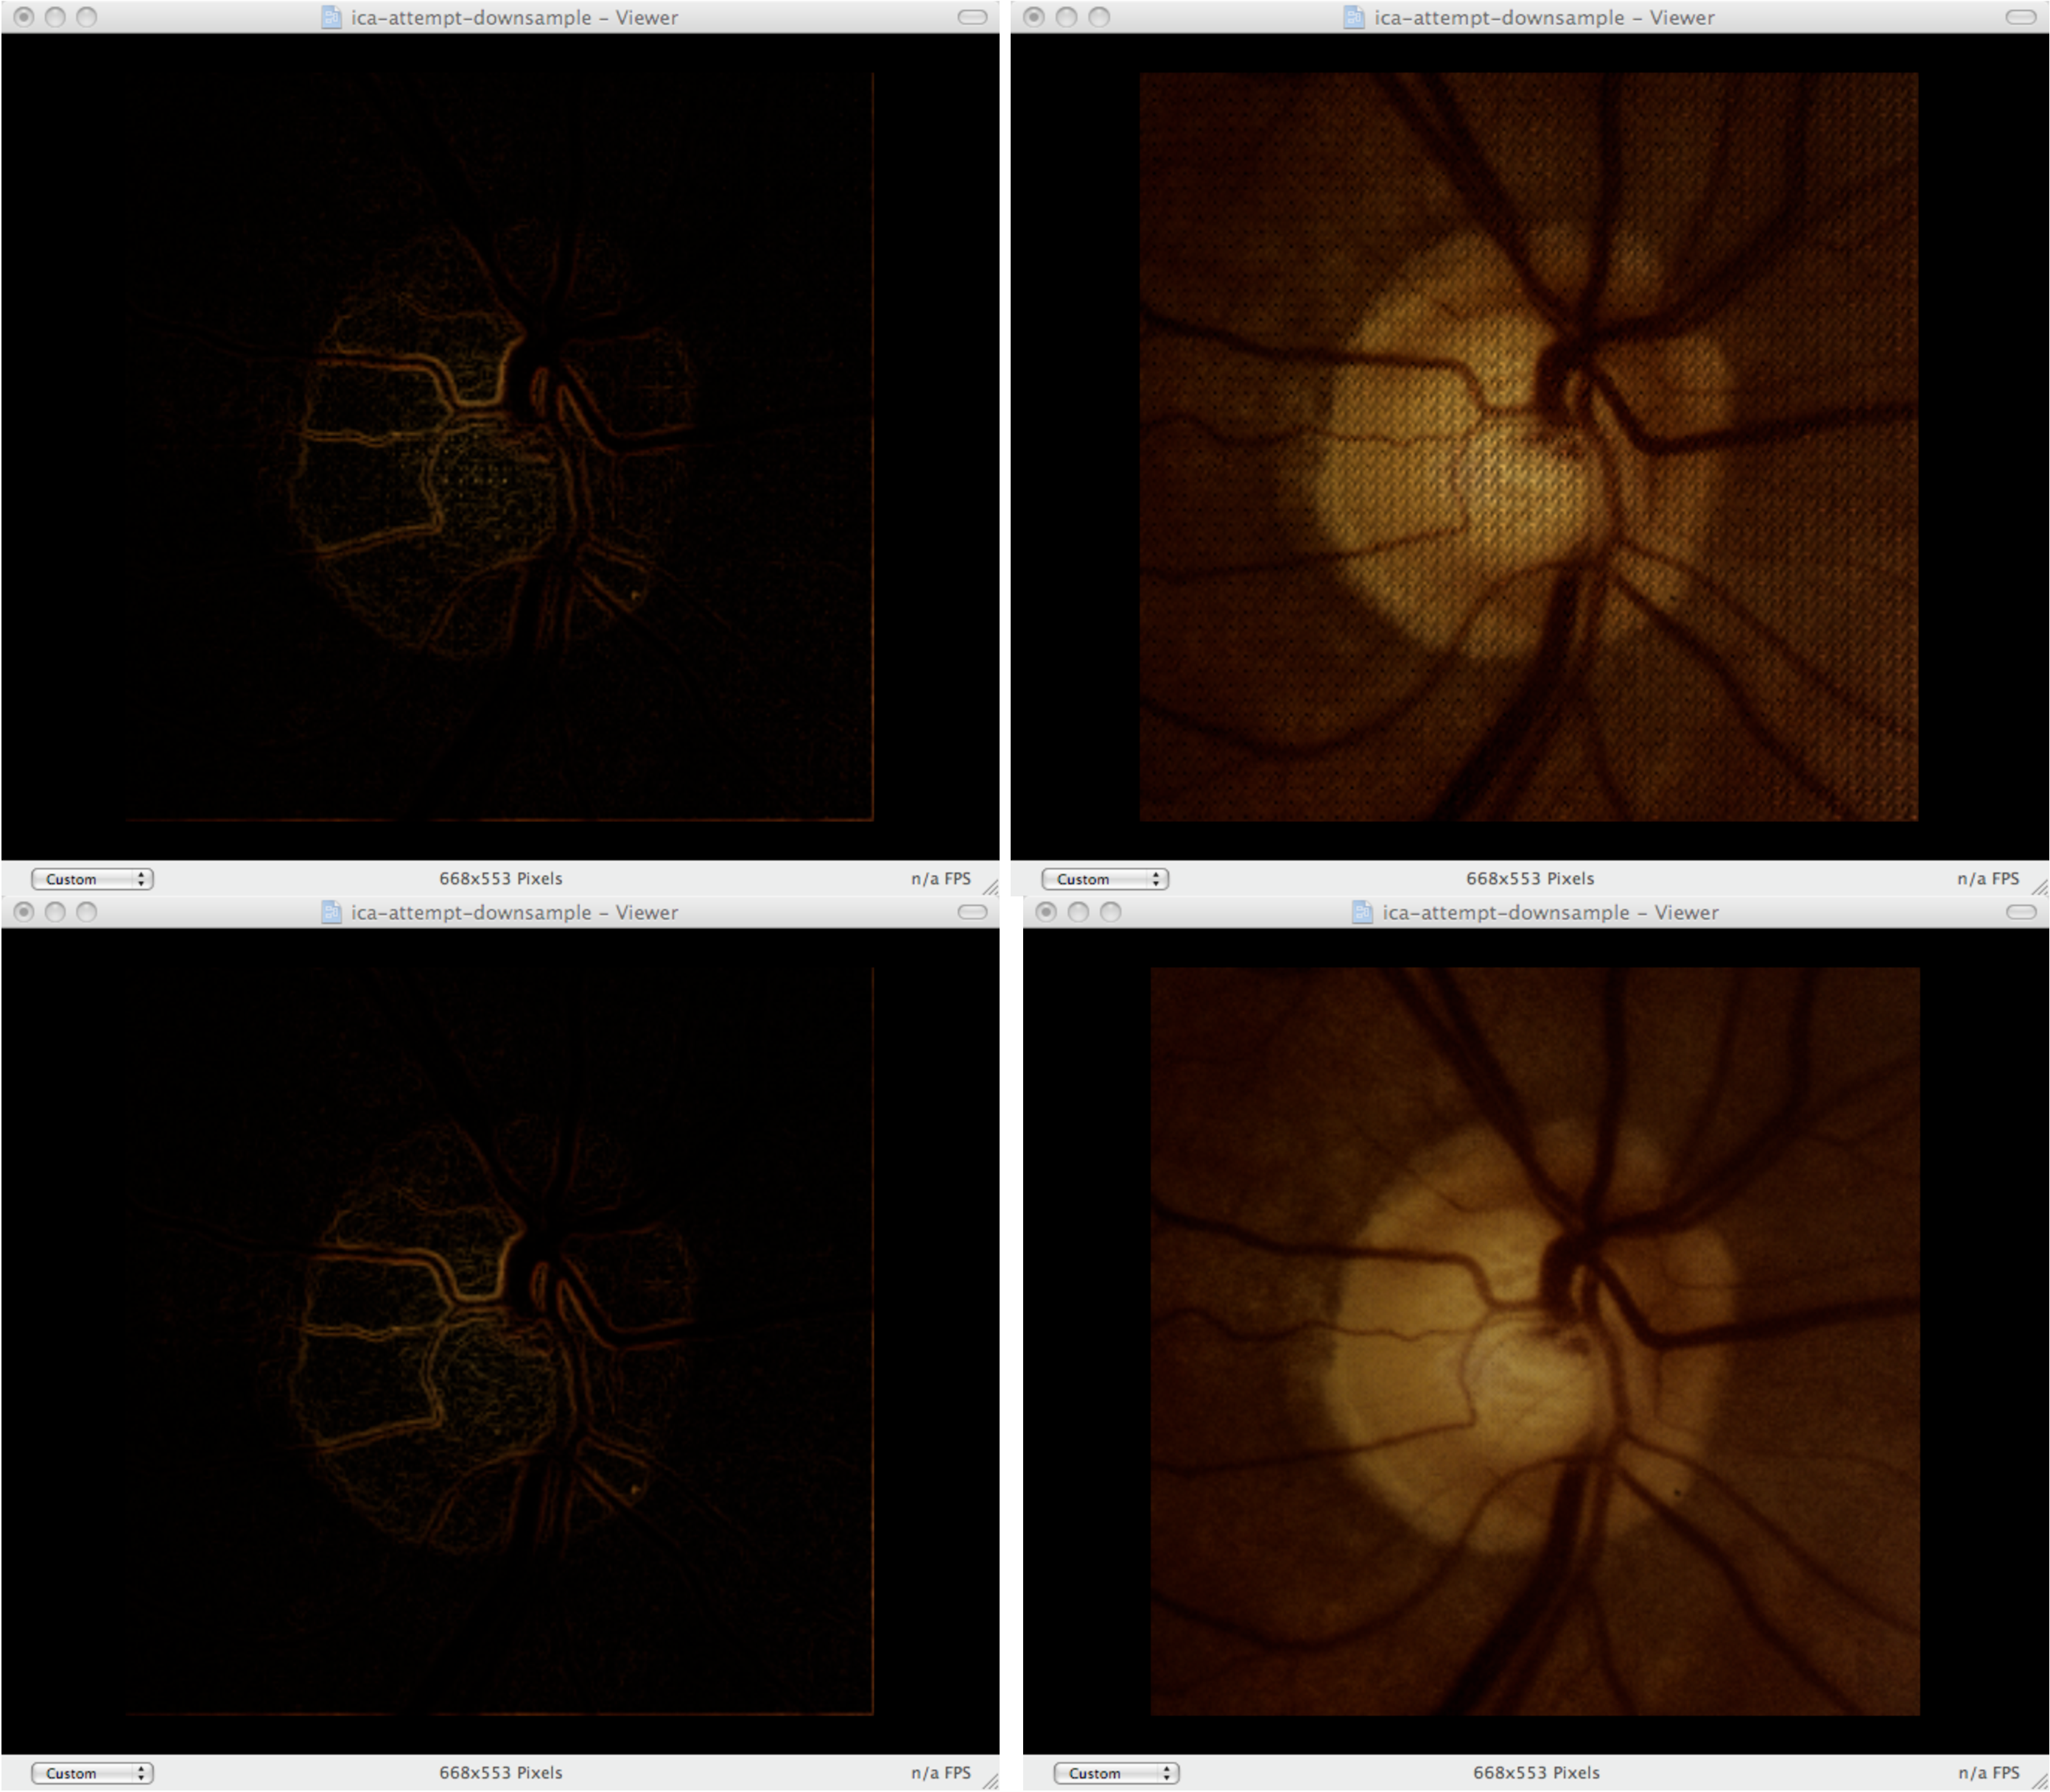
\includegraphics[width=6in]{ica-downsample-eye.pdf} 
   \caption{This is a set of results of a Quartz Composition of a ICA-Downsample.  In this sample, the red channel is the primary source for the PCA-ICA estimator.  On the left, an edge filter is applied before the image is channelled %the image 
into the PCA-ICA estimator.  The results are multiply blended with the original image.  On the right, the original image is multiply blended with the PCA-ICA estimation. }
   \label{downsampled-ica-quartz-composer-red-channel}
\end{figure}




\section{A Core Image Innovation}
As mentioned in the mathematical background section, there is another way to compute the mixing matrix for determining principal components, namely Gram-Schmidt Orthogonalization.  In CPU form, the iterative nature of EVD and SVD.

\subsection{Pseudo Zero Branch Program Model}
%Why Turing Complete Requires Branch
Turing's theorem inherently requires that a computational models include branches or more precisely have a form of recursion.  In the simplest form, recursion is defined in terms of multiple stacks.  The concept of recursion allows for a finite number of instructions to be repeated many times to accomplish an otherwise complex result.  Models for recursion were developed that specify that any construct conforming to a safe recursion model will in fact complete its task.

%Trouble for vector engines
Vector engines have trouble with branches.  %The reason for this trouble 
Trouble occurs in the construction of such engines and is rooted in the key engine mechanism, which is the pipeline.   Pipelines are designed with the same philosophy as a commonly known concept called the assembly line.  Each stage of the pipeline carries out a portion of the work, and each stage works simultaneously.  The consequence of this model is that one result is produced per stage execution (after the pipeline is filled).   Many CPU models have this concept,  and there are  compilers for these models that optimize programs for these pipelines.  Because CPU models are  general purpose machines there are limits of how large pipelines can be while satisfying the branch requirement.

A GPU favors the pipeline model over branches by necessity.  In order to provide the billions of operations per second necessary for responsive renderings, a GPU must include pipelines optimized for determining each two and three dimensional points.   In these cases, a program that has no branches of any kind is called zero-branch.  

%If no branches in the main process, then where?  -- Hybrid Approach 
There is a hybrid approach between CPU and GPU models that can generate modules which are zero-branch.  The hybrid uses modules which are themselves zero-branch and are optimized for the GPU.  The CPU furnishes the branches necessary to combine each module into a structure satisfying the desired calculation.  The result of this hybrid approach is that the CPU builds zero-branch programs to be executed on the GPU.   Optimization of this hybrid approach becomes a function of well chosen modules, the reuse of constructed modules, and a parallel construction of reused modules.  


\subsection{Core Image Kernel Model}
%What is a Core Image Kernel
The Core Image (CI) Kernel Model (CIKM) satisfies the requirement for modules that are themselves zero-branch programs.  A Core Image Kernel is a zero-branch program which is defined in terms of each pixel in a defined region of interest (ROI).  The language used to construct Core Image Kernels, Core Image Kernel Language (CIKL), is a subset of Silicon Graphic's OpenGL's Shading Language (GLSL), which is built on a similar philosophy.   CIKL restricts branches to those which can be determined at compile time.   The output of each kernel is an image, and the input types include images, scalar numbers and four element vectors.  

A ROI is specific set of points (pixels) by which a kernel may operate on.  There may be multiple ROI, one for the destination image and one for each input image.   A CI Filter object provides a region of interest which may be overwritten to specify a ROI for each input image.  The ROI for the destination is specified on the call of the CI Kernel itself, which by convention of the construction of CI Filters is invoked inside of the output image method.  

%What provisions exist for CI
CIKL includes a compare instruction.  This compare instruction is not a branch instruction.  It simply provides one of the two provided values based on the less than operation included in the instruction. The compare operation compares, in the scalar case,  an input denoted $x$, and returns either the second input, $y$, if $x < 0$ and the third input, $z$, otherwise.  The vector version performs the selection on each element of the vectors $\vec{x}, \vec{y}$, and $\vec{z}$ respectively.
%CIKL also provides basic mathematical syntax for performing scalar and dot vector operations (limited to the 2, 3, and 4 elements).  Two element vectors are used to define coordinates in images.  Four element vectors used to define the individual color values of the image (pixels).  

Each kernel function is defined in terms of each of the input vectors, scalars, image samplers, and  destination pixel, whose coordinate is given by the destination coordinate function (destCoord()).  Any of point in an input image sampler may be accessed through the ``sample'' function.  It is typical to define a kernel which isolates the specific point in the input samplers and performs some fundamental mathematical operation on these points.  Mathematical operations include scalar and dot vector versions of  trigonometric operations (cosine and sine), addition  subtract, multiply, division, and modulus.    

%How is the computation model defined?
No destination pixel can be reused as an input pixel for the kernel itself.  This would force an order dependency which is not supported in the CIKM.  In order to perform such operations, one kernel may supply its output image as an input image to another, as shown in sub-section \ref{cifiltergenerator}. Each of the points are determined in parallel via the vector pipelines, which are specified in the GLSL specification.  The kernel then becomes a pipelined structure, and provides the efficiency of the CIKM.  

\subsection{Constructing Where Size and Position Matters}\label{cifiltergenerator}

%CI Filter Generators fundamental connection
As stated the results of a CI Kernel can be used as an input to another CI Kernel.  The CI Filter object encapsulates each respective CI Kernel.   In principal, any loop can be used to insert images, both original and outputs of CI Filters, into more CI Filters.   This process can  encapsulate and define complex filters using what is called a CI Filter Generator.  A CI Filter Generator provides a connect object method to connect one CI Filter, number or vector to another CI Filter, and form a structure of these connections.    The structure itself is capable of forming an archive which can be saved and passed on to other processes.      

%What they export
This structure can also be used to construct another CI Filter.   Such a CI Filter is the compilation of the CI Filter Generator's member filters.   The definition of the CI Filter is determined by the way each member filter is connected. % connection of filter in the CI Filter Generator defines the specifics of the constructed filter.  
The resulting filter is a stored object which the CIKL compiler constructs into a concise filter.   The resulting filter constructed by a CI Filter Generator can be used by another CI Filter Generator.  

%Where they define their meaning
Thus a CPU-bound loop can assemble any complex CI Filter through a CI Filter Generator instance from less complex filters.  It is typical to define the inner loop of a particular process as a CI Filter (constructed by a CI Filter Generator instance), then use a CPU bound loop to connect each inner loop filter to each other.  The just-in-time compiler determines the dependencies and how many pipelines are needed to perform the computation optimally.  

%How they export
There are special items in addition to the connecting filters that define a CI Filter Generator's output filter.  Each CI Filter Generator supplies a dictionary defining the name, description and other special attributes of the constructed filter.  Also, each CI Filter Generator supplies export keys to define the input ports and output image of the resulting CI Filter.  


\subsection{GSO version of PCA using the Core Image Kernel Model}
% identify the QC plug-in solution
The CIKM solution for determining PCA is solved by solving GSO through a CIKM model.  This solution requires eight filters.  Of the eight filters, three are kernels supplied by the DC lab, six are generated as a combination of the three kernels, and three of the six can be computed in parallel without difficulty.  

In the process of generating a CIKM solution, the orientation of the solution is kept in neighborhood form, which alters the orientation of the operations needed to produce the GSO super-kernel.    The add image and dot multiply stay the same, as there are no cross products in either of these kernels.  The computations of the norms, inner products, column scales, and column subtractions take on a new form.  

\begin{figure}[htbp] %  figure placement: here, top, bottom, or page
   \centering
   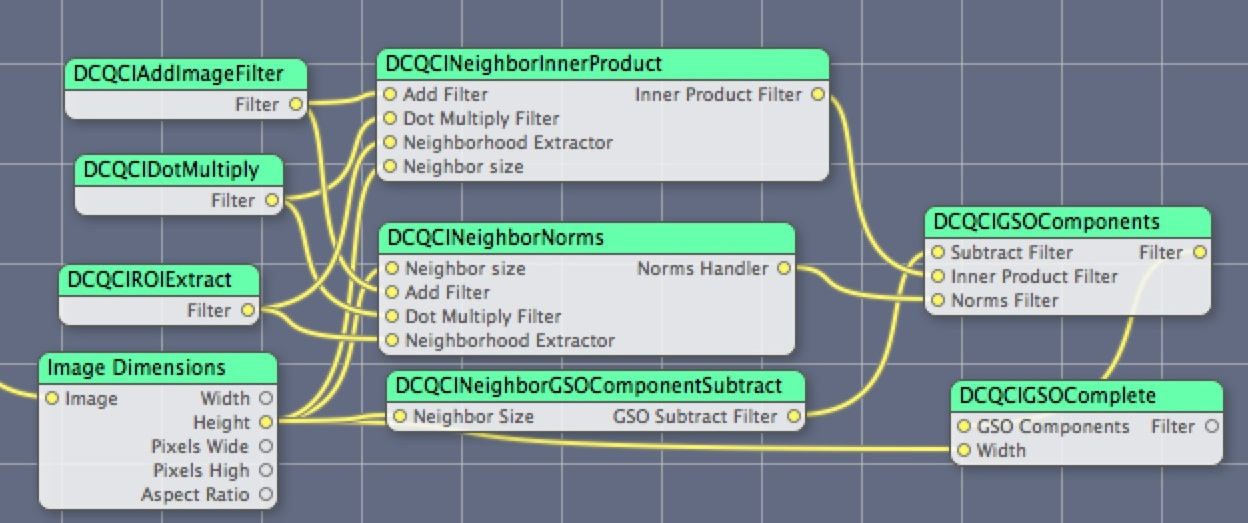
\includegraphics[width=5in]{gso-qc-fundamental-core.jpg} 
   \caption{These are the core filters required for GSO.  They are computing in this case by a pseudo-algebra called in this report neighborhood algebra. }
   \label{qc-gso-fundamental-core}
\end{figure}


\begin{figure}[htbp] %  figure placement: here, top, bottom, or page
   \centering
   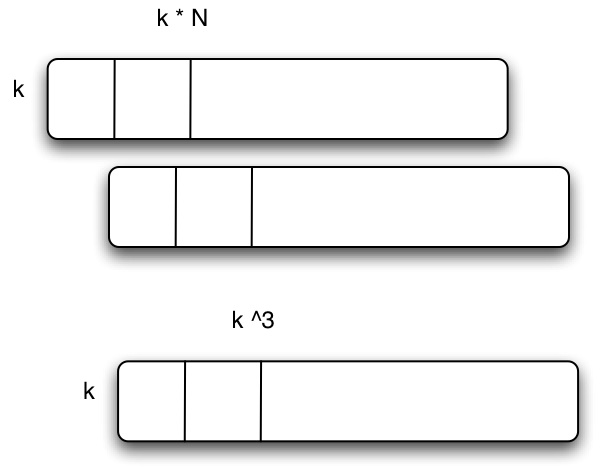
\includegraphics[width=5in]{neighborhoodArrangement.jpg} 
   \caption{This diagram shows the arrangement of neighborhoods in a neighborhood mixing image. }
   \label{neighborhoodArrangement}
\end{figure}

\subsubsection{Neighborhood Orientation to Linear Algebra}
The mathematics associated with this neighborhood orientation is called, in this report, neighborhood algebra.   A neighborhood is treated as analogous to a column vector in standard linear algebra.  A neighborhood is a $k \times k$ image extracted from the image itself.  Neighborhoods are arranged horizontally forming a $k \times kN$ image where $N$ is the quantity of neighborhoods, which is shown in Figure \ref{neighborhoodArrangement}.  %This choice is made based on neighborhood nature of filtering, and inherent properties of ROI structures.  
A third kernel filter produced for this report, which crops and translocates specific neighborhoods, is ROI extract, which copies out a region of interest as the name implies.  This neighborhood orientation has advantages in image processing operations.  Dot multiply and addition are simpler operations than full matrix multiply, which is an example of the motivation for this neighborhood orientation.   


GSO is an example of a linear algebra operation that benefits from neighbor orientation, and becomes a means of achieving parallelism in the construction of the CIKM generated filter for GSO.   The generated filters are shown in Figure \ref{qc-gso-fundamental-core}.   The inner product, norms, and neighborhood scale with subtract (GSOComponentSubtract in the figure) handlers can each be determined independent of each other.  Their generator connection diagrams are shown in Figures \ref{neighborhoodInnerProduct}, \ref{neighborhoodNorms}, and \ref{gsoSubtract}.

\subsubsection{Reductions resulting from ``Neighborhood Algebra''}
Inner products computed in these cases reduces to one dot multiply between two neighborhoods, followed by $k$ sums.   Norms of the neighbors is one dot multiply, and $k$ sums of the elements inside each neighborhood. The scale and subtract is even more straight forward.  The scaling operation dot divides the inner product image by the norm image.  The resulting image is used to scale each neighborhood via the neighborhood scale kernel filter.  The final subtract filter subtracts a selected neighborhood from the working neighborhood and repeats this process for each neighborhood in the mixing image.  The caveat of the scale and subtract filter is that the neighborhoods in the scaled mixing image from the working neighborhood to the right are zeroed.  This allows for the scale and subtract to be general for each inner loop.  


% Neighbor space 
% Inner product 


\begin{figure}[htbp] %  figure placement: here, top, bottom, or page
   \centering
   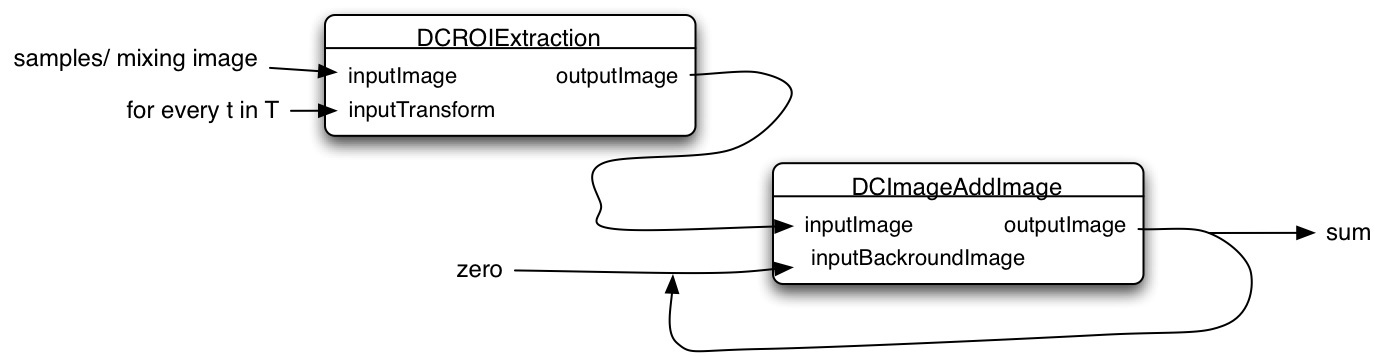
\includegraphics[width=5in]{neighborhoodSum.jpg} 
   \caption{This diagram shows the connection of fundamental kernels to form a neighborhood sum kernel. }
   \label{neighborhoodSum}
\end{figure}


\begin{figure}[htbp] %  figure placement: here, top, bottom, or page
   \centering
   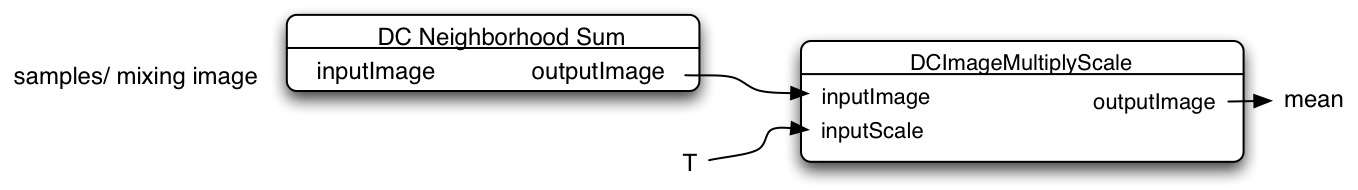
\includegraphics[width=5in]{neighborhoodMean.jpg} 
   \caption{This diagram shows the connection of fundamental kernels to form a neighborhood mean kernel. }
   \label{neighborhoodMean}
\end{figure}



\begin{figure}[htbp] %  figure placement: here, top, bottom, or page
   \centering
   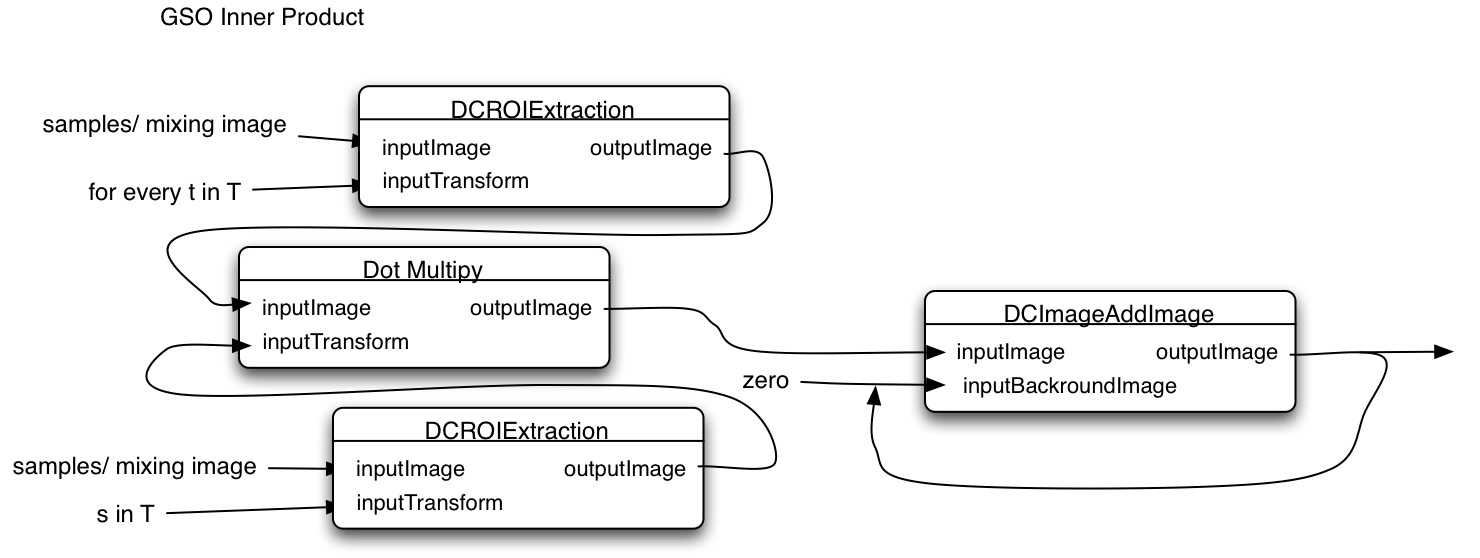
\includegraphics[width=5in]{neighborhoodInnerProduct.jpg} 
   \caption{This diagram shows the connection of fundamental kernels to form a neighborhood inner product kernel. }
   \label{neighborhoodInnerProduct}
\end{figure}


\begin{figure}[htbp] %  figure placement: here, top, bottom, or page
   \centering
   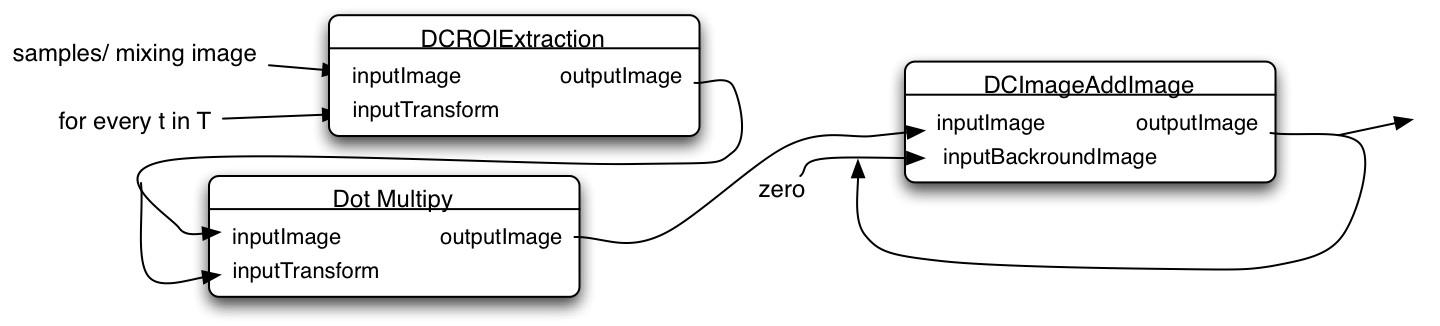
\includegraphics[width=5in]{neighborhoodNorms.jpg} 
   \caption{This diagram shows the connection of fundamental kernels to form a neighborhood norms kernel. }
   \label{neighborhoodNorms}
\end{figure}


\begin{figure}[htbp] %  figure placement: here, top, bottom, or page
   \centering
   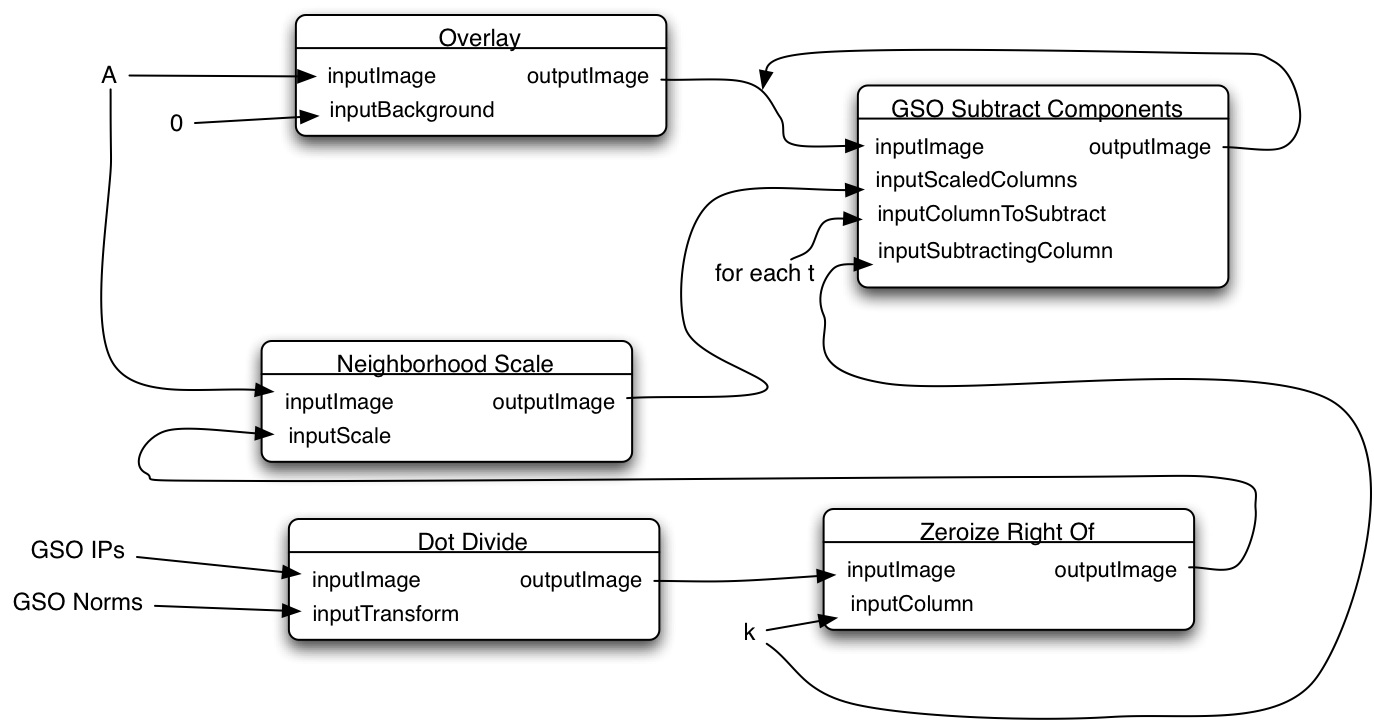
\includegraphics[width=5in]{gso-subtract.jpg} 
   \caption{This diagram shows the connection of fundamental kernels to form a neighborhood subtract kernel. }
   \label{gsoSubtract}
\end{figure}


\begin{figure}[htbp] %  figure placement: here, top, bottom, or page
   \centering
   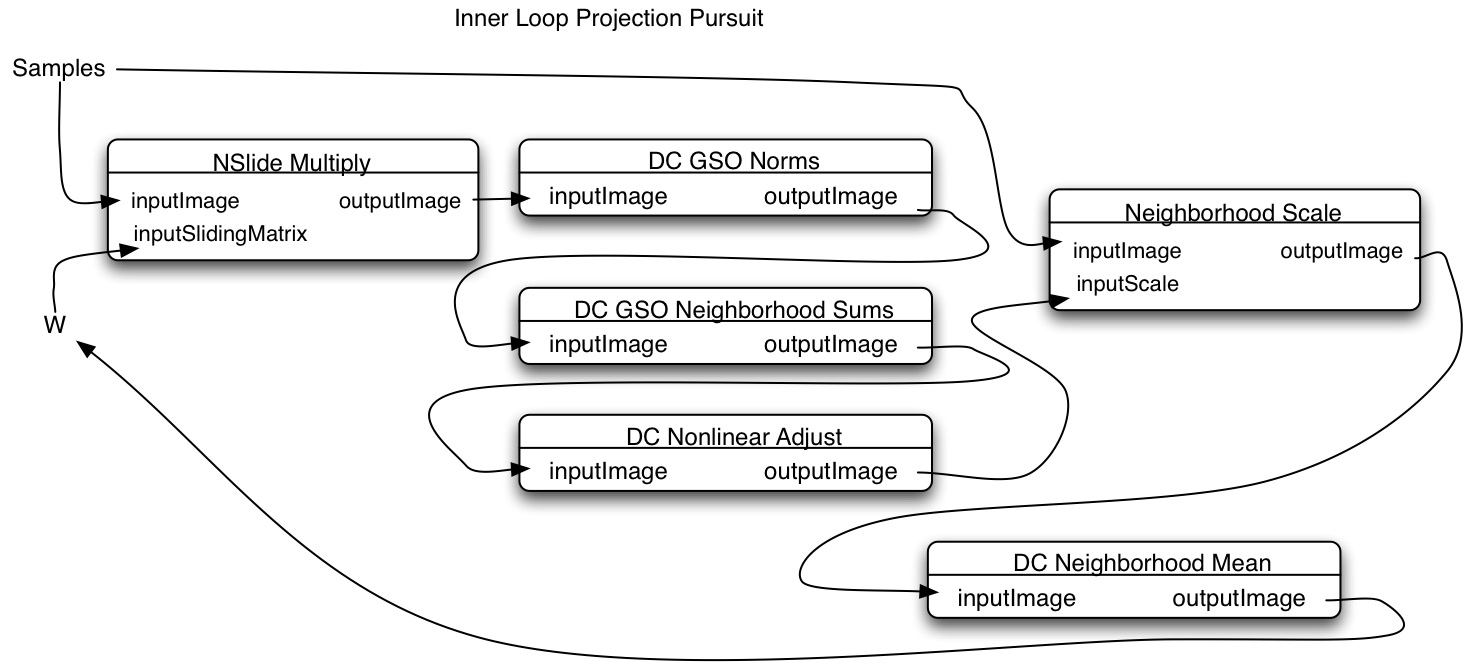
\includegraphics[width=5in]{neighborhoodICA.jpg} 
   \caption{This diagram shows the connection of fundamental kernels to form a neighborhood ICA kernel. }
   \label{neighborhoodICA}
\end{figure}

\subsection{Debugging GPU-bound products using Quartz Composer}
%What is Quartz Composer?
Quartz Composer (QC) is a rapid development environment tool that allows a developer or user to use concise units, called patches, to construct powerful graphics oriented effects.  QC provides the user with a set of filters, generators, input patches, composite patches and plug-ins to construct effects while contributing very little program code.  The plug-in patches and SDK provides developers the ability to test their own code, which they provide in an intuitive manner.  QC was shown in the CPU-bound implementations of PCA and ICA in this report.  

%What are Quartz Composer plug-ins 
In this sub-section, QC plug-ins are further elaborated to aid in understanding QC's prototype assisting power.  In both cases, developing a CPU-bound filter and a CIKM filter, the dictionary type (NS-Dictionary ) is key to moving these data-types from patch to patch.  This particular dictionary type can store any object type, and it is useful to pair that object with a standardized key.  In the case of CIKM types, the key used is ``CIFilter,'' which is the precise data type used and produced.  

Also in this sub-section an incremental approach is made by reducing the QC Plug-in to a loop controller with feedback.  This concept allows kernel level CI Filters to be connected directly in QC without using a dictionary as a wrapper.  The advantage is that the prototype is reduced in complexity.  The disadvantage is rooted in the selection and copy of either the feedback or initial images.  

\subsubsection{Excessive Handlers: Debugging the generator and filters}
 
Each QC plug-in constructing a CIKM filter has the same output type, a CI Filter wrapped in a dictionary.  The input for these plug-ins are dictionaries containing composing filters, and double-floating point real numbers representing the constants needed to construct the filter.   
The execution of the plug-in determines if there has been a change in the input, and proceeds if there has been.  
If the inputs are appropriate for the filter handler, which is an object that contains the method and objects necessary to construct the combined filter, then the handler returns an object, and nil otherwise.  If the result is nil, then the output is also assigned nil and the execution is reported with a value of ``NO''.  If the handler is not nil, then the handler is instructed to determine the filter, and the filter is assigned to the output dictionary.

%Using QC Patches to connect rudimentary filters into generating handlers.

Each handler initialization method takes in the input parameters necessary to construct the desired filter.  There are four filter types that handler can use.  A filter produced by another handler is one of the types, and by convention, is one that should be a property of the handler.  The second type is a standard CI filter, which is included with the CI package for which there are many  supplied by Apple, Inc.  Another set of CI filters  are those supplied by the Distributed Computing Lab (Texas Tech University) as part of the DC frameworks.   Lastly, more handlers and filters could be constructed by third parties.

Each handler contains a method, called ``determine,'' which uses the CI Filter Generator to connect each of the supporting filters.  There is a safeguard in the event that the ``determine'' method fails.     If the output dictionary is not nil, then the execution is reported as ``YES,'' otherwise ``NO'' is reported.  The ``NO'' tells Quartz Composer that something is wrong and causes any patches in the execution path to stop.  

Lastly, there is one special QC Plug-in that can only use the handler for connecting  attributes to an input filter.  This QC Plug-in family is called an imposition plug-in.  Its purpose is to apply the generated filter to an actual image.  This type of plug-in is built for a specific type of QC patch, which is for the final filter.   As such, the patch possesses as input ports the filter itself and the filter's inputs (images, numbers and vectors).  The output must be a QC image. %, and should primarily use the texture orientation.  


\subsubsection{Reducing debugging problems by using QC-Plug-in to Control the Loop}

There are benefits from the control loop model. First, the prototype reduces all CI Filters to kernel level.  Each patch can be reduced to unit purpose. Each unit purpose patch has a direct resemblance to its neighborhood algebra model. Lastly, the native CI patch can be used to reduce the CI Filter plug-in's, reducing the number of filters necessary to distribute.  
	
The inner loop of GSO in this feedback control loop model obeys the neighborhood algebra model.  The inner product and norms results are fed into the subtraction composition.  The input to both inner product and norms compositions are either the initial image or feedback from the subtract composition.  The loop and determination of the input to the inner loop is controlled by the feedback and control plug-in.  

The inner product composition also obeys the neighborhood algebra model and has a feedback control patch.  The same can be said about norms and the subtraction composition.  As the neighborhood model specifies the number of neighborhoods is the ratio of width to height, the dimensions' patch in combination with a math patch determines these values.   These patches can be observed in Figure \ref{controlLoopGSO}.   

\begin{figure}[htbp] %  figure placement: here, top, bottom, or page
   \centering
   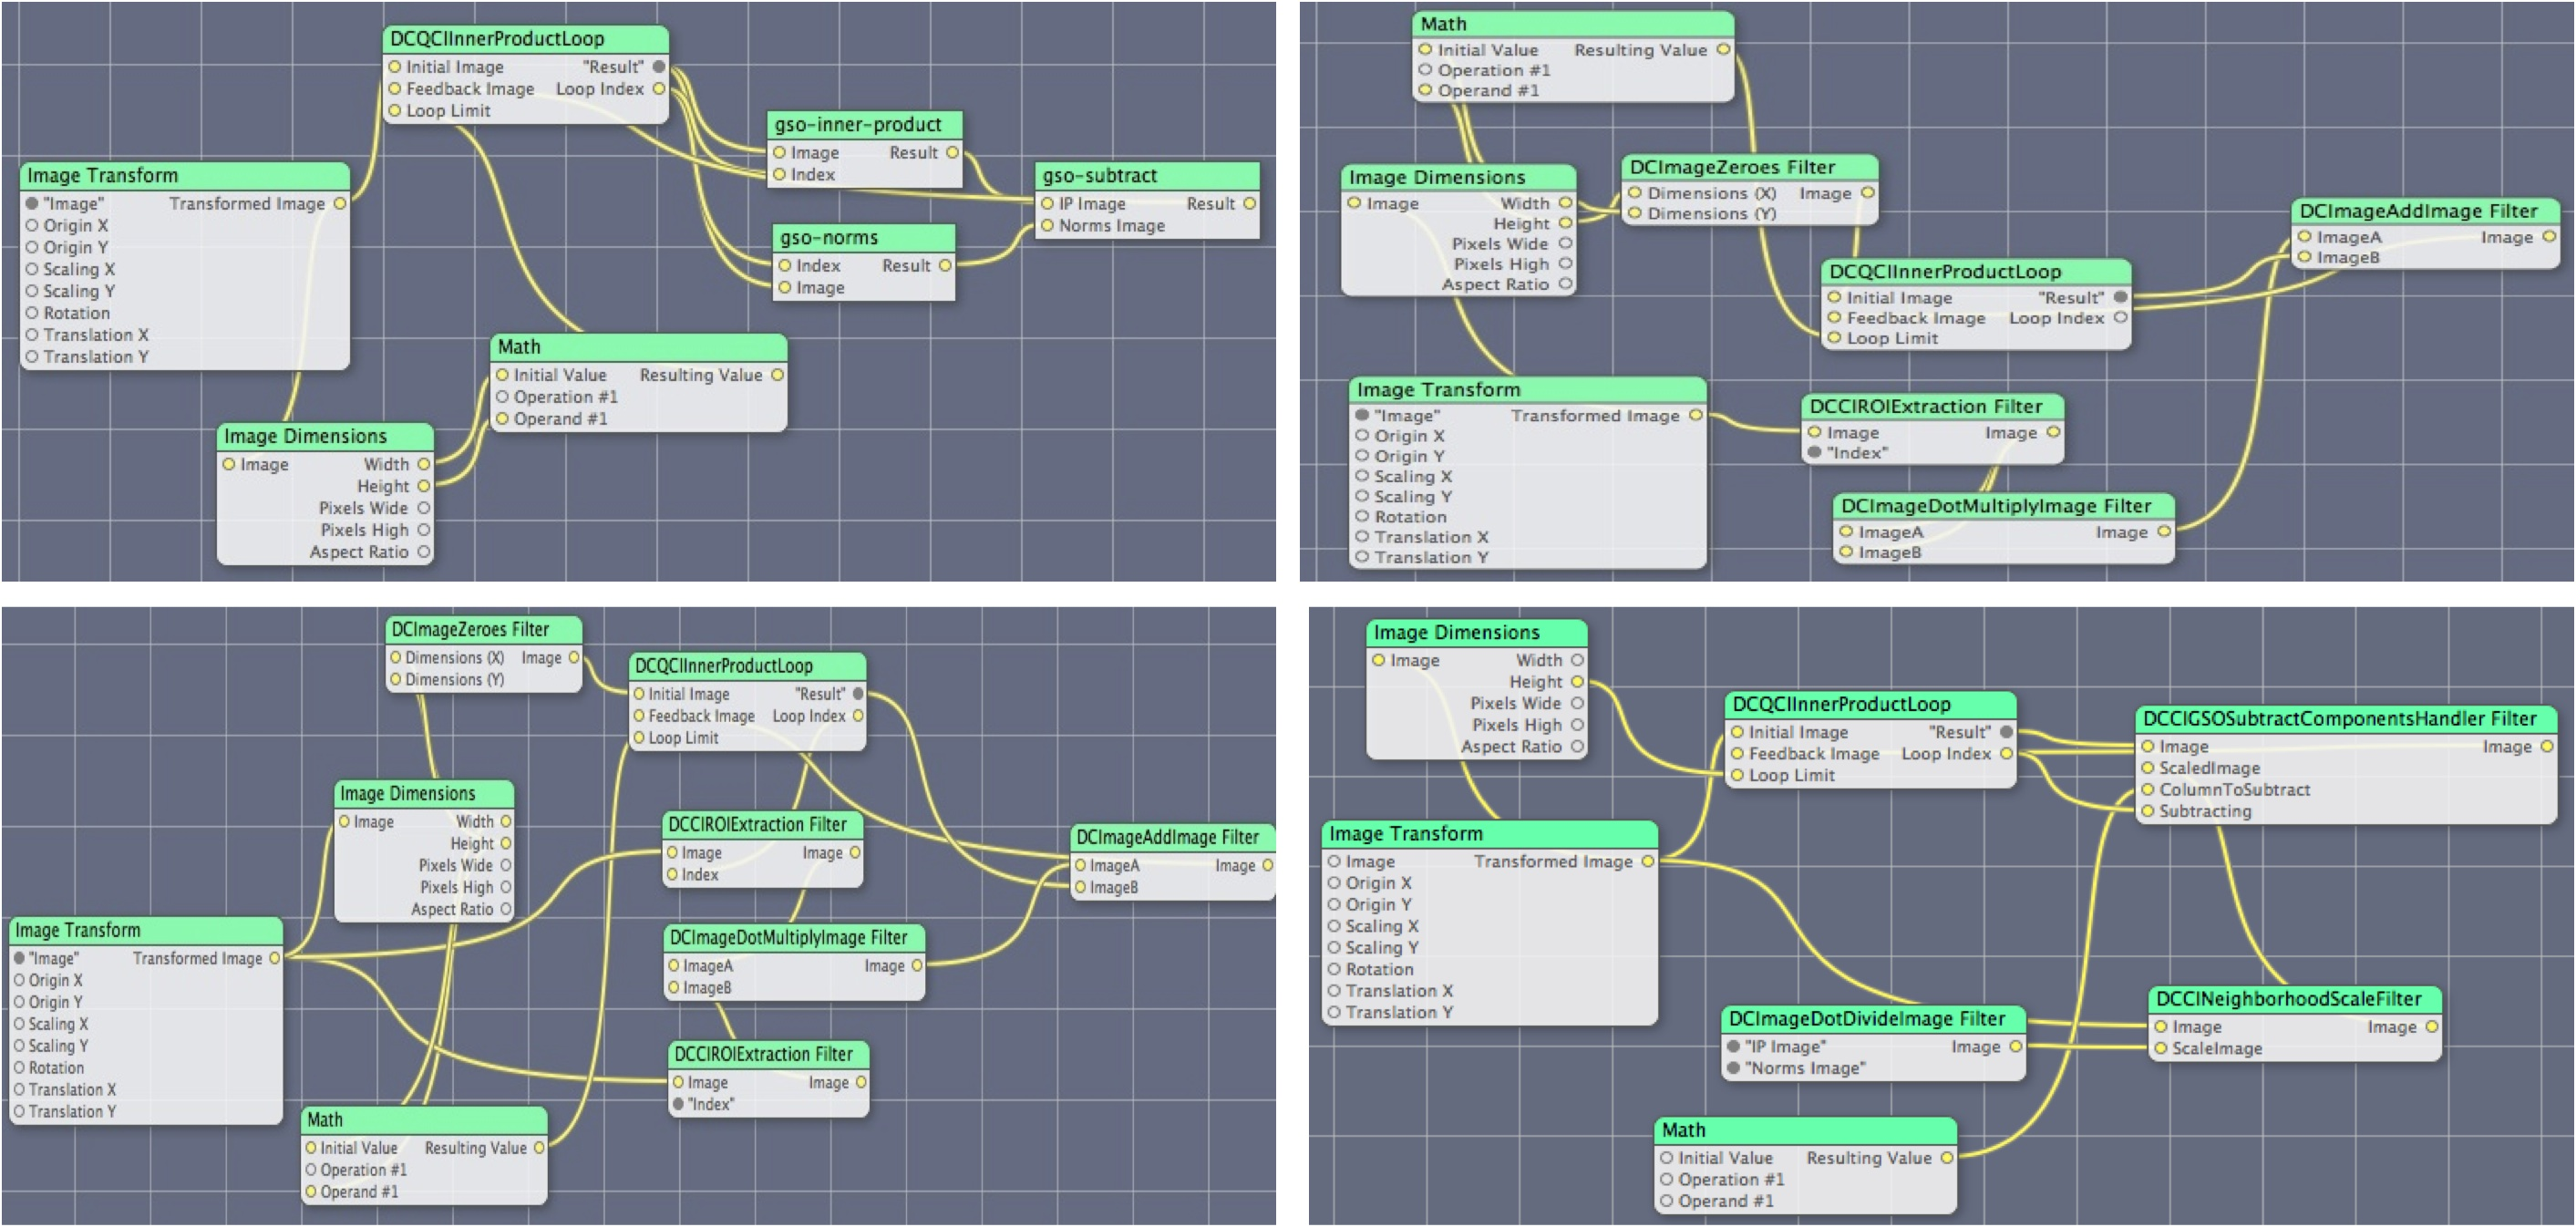
\includegraphics[width=6in]{controlLoopGSO.jpg} 
   \caption{This diagram shows the collection of QC patches computing GSO using a feedback control patch.  Called DCQCIInnerProductLoop in these diagrams, the control patch provides a mechanism for feedback to build a solution for the PCA mixing matrix.  This approach empowers QC to provide prototyping tool for GPU bound solutions.}
   \label{controlLoopGSO}
\end{figure}

The feedback control loop itself has three inputs.  The two images, initial and feedback, supply the control with a selection to start and finish the loop.  The loop limit controls how many loops may be executed.  This works well with the neighborhood algebra model as it is typically the height of the image being computed.  The outputs of the feedback control loop patch are the result image and the loop index.  The result image is fed into the compositions components, which define the unit's inner loop.  The loop index, as the name implies, is the index for the inner loop's components to work on.   This is a consequence of the neighborhood algebra model and does have a design pattern to it.  
	
The GSO version of PCA produces a similar mixing matrix to the EVD-PCA method.  In this case, neighborhood expansion and selection can solve segmentation problems.  Also, use of neighborhood expansion and scaling can solve noise reduction problems. 
	
There are some caveats with using the QC Plug-in control loop implementation of the neighborhood algebra model of GSO-PCA. The Loop controller itself has to copy the image from input to output protocols.  A limit exists in these protocols for texture and buffer resolution. 
Perpetual build and stop means that the solution is eventually reached, and the intermediate values are seen too.  



\subsection{Accelerate Construction using NSOperation}\label{nsoperation-for-cifilter-generator}
There is a method for altering a handler, originally made for a Quartz Composer plug-in, to inherit multi-threaded properties by making it a NS-Operation subclass. % to being a subclass of NSOperation, which inherits multi-threaded properties.  
There are three key differences which do not effect the logic, but supply parallelism to the computation.  First the algorithm specified in the ``determine'' method becomes the ``main'' method.  Second, the properties passed by other handlers must be accessed from the other handlers and the other handlers become dependent properties of the operating handler.  These handlers must be specified as dependencies.  Third, the handlers become operations themselves, and those operations must be loaded into an NS-Operation Queue while the queue is suspended.   Once loaded, the queue may be reactivated, which causes the handlers to be determined in parallel fashion.  
%One key to that transformation is making the determine method the main method, and altering the input filters to being handlers that generated them.   The other part is to stop the NS-Operation queue while loading operation objects into the queue.  

% Basic Loop concept 

% Proper use of feedback 

% Issue of in and out protocols for QC-Plugin images.  


% Neighborhood algebra


% Norms 
% Dot divide 
% Neighbor scale
% GSO Subtract

% Neighbor expansion
Figure  \ref{qc-gso-fundamental-core} shows the Quartz Composer patch connection method of combining these filter generating handlers.  The filters can be converted to NS-Operation subclasses with relative ease.  This conversion allows for a NS-Operation Queue to determine the final filter.  There are two possibilities of deployment via this queue.  The queue can be inserted into a CI-Filter plug-in as a CPU component of the filter.    The advantage of the pseudo filter is that it is usable in Quartz Composer and is treated as a kernel filter. This is sort of  pseudo filter can have one disadvantage.  The disadvantage is the filter may not be reused without being regenerated.  Also, the filter does have to wait for the queue to finish computations.  On single CPU systems, that queue could take more time than the security model allows.   


% Show the handler construction

% identify the problem for QC

% QC: Use plug-in patches to form the loop control, and use feedback to perpetuate the inner loop. 

%  Show the non-threaded gerneration.

%  Show the NS-Operation version


\appendix


\section{A Listing Mathematica Implementation for the Iris Data-set}
\label{listing-mathematica-iris}
\begin{lstlisting}{language=Mathematica}
barSetosa = Mean[setosa]
barSetosaArray = PadLeft[{barSetosa}, First[Dimensions[setosa]], {barSetosa}]
normSetosa = setosa - barSetosaArray
ScatterSetosa = Transpose[normSetosa].normSetosa/First[Dimensions[setosa]]

barVersicolor = Mean[versicolor]
barVersicolorArray = PadLeft[{barVersicolor}, First[Dimensions[
  versicolor]], {barVersicolor}]

normVersicolor = versicolor - barVersicolorArray
ScatterVeriscolor =
         Transpose[normVersicolor].normVersicolor/First[Dimensions[versicolor]\
]

barVirginica = Mean[virginica]
barVirginicaArray = PadLeft[{barVirginica}, First[Dimensions[virginica]], \
{barVirginica}]
normVirginica = virginica - barVirginicaArray
ScatterVirginica = \
Transpose[normVirginica].normVirginica/First[Dimensions[virginica]]
whiteningScatter = ScatterVirginica + ScatterSetosa + ScatterVeriscolor
flowers = Join[setosa, versicolor, virginica]
combinedMean = Mean[flowers]
flowers = Join[setosa, versicolor, virginica]
combinedMean = Mean[flowers]
meanArray = Join[{barSetosa}, {barVersicolor}, {barVirginica}]
combineMeanArray = PadLeft[{combinedMean}, Dimensions[meanArray], \
{combinedMean}]
meanDifference = (meanArray - combineMeanArray)
scatterBackground = Transpose[meanDifference] .(50*meanDifference)
{lambda, W} = Eigensystem [{scatterBackground, whiteningScatter}, 2]
ListPlot[flowers.Transpose[W]]
\end{lstlisting}

\section {A Listing of the Objective-C version of EM}


\begin{lstlisting} [ language={[Objective] C} ,caption={Initialize EM}, label=lst_initializeEM ] 


-(id) initWithSamples:(dcgVector *) someSamples
					numberOfGaussians:(int) M
{
	[super init];
	numberOfClasses = M;
	numberOfSamples = [someSamples vecLength];
	samples = [someSamples retain];

	double max = [samples max];
	double min = [samples min];
	
	double scale = (max - min)  / M ;
//	scale *= 0.5;
	int r;
	
	mean = [[dcgVector alloc] initWithLength:numberOfClasses];
	variance = [[dcgVector alloc] initWithLength:numberOfClasses];
	proportions = [[dcgVector alloc] initWithLength:numberOfClasses];
	mixture = [[dcgMatrix alloc] initWithRows:numberOfSamples
					columns:numberOfClasses
					];
	double *mu = [mean localVector];
	double *sigma = [variance localVector];
	double *alpha = [proportions localVector];
	
	for ( r = 0; r < M; r++) {
		mu[r] = (max - min ) * r * scale + min ;
		sigma[r] = scale;
		alpha[r] = scale;
	}

	[self computeEM];
	return self;
}					

\end{lstlisting}

\begin{lstlisting} [ language={[Objective] C} ,caption={Estimation step of EM, computed explicitly in Objective C}, label=lst_estimationStepEM ] 

-(void) estimationStep
{
	double *mu = [mean localVector];
	double *sigma = [variance localVector];
	double *alpha = [proportions localVector];
	double **A = [mixture localMatrix];
	double *D = [samples localVector];
	
	double amp, sumAlpha = 0;
	Q = 0;
	int r, c; 
	
	for ( r = 0 ; r < numberOfSamples; r++)
		for ( c = 0; c < numberOfClasses; c++)
		{
			amp = alpha[c];
			amp /= sqrt(2 *M_PI * sigma[c]);
			A[r][c] = amp * exp (-0.5 * (D[r] - mu[c])  * (D[r] -mu[c]) / sigma[c]) ;
		}
		
	for ( r = 0 ; r < numberOfSamples; r++)
	{
		sumAlpha = 0;
		for ( c = 0; c < numberOfClasses; c++)
			sumAlpha += A[r][c] ;
		for ( c = 0; c < numberOfClasses; c++)
			A[c][r] /= sumAlpha ;
	}
	
	for ( r = 0; r < numberOfSamples; r++) 
	{
		 sumAlpha = 0.0;
		 for ( c = 0; c < numberOfClasses; c++)
			sumAlpha += A[r][c] ;
		 Q += fabs(log(sumAlpha));
	}
		
	
}

\end{lstlisting}


\begin{lstlisting} [ language={[Objective] C} ,caption={Maximization step of EM, computed explicitly in Objective C}, label=lst_maximizationStepEM ] 

-(void) maximizationStep
{
	double *mu = [mean localVector];
	double *sigma = [variance localVector];
	double *alpha = [proportions localVector];
	double **A = [mixture localMatrix];
	double *Y = [samples localVector];
	
	int r, c; 
	double meanDifference;

	
	[proportions zeroize];
	for ( r =0; r < numberOfSamples; r++) 
		for ( c = 0; c < numberOfClasses; c++)
			alpha[c] += A[r][c];
	
	[variance zeroize];
	for ( r =0; r < numberOfSamples; r++)
		for ( c = 0; c < numberOfClasses; c++)
		{
			meanDifference = Y[r] - mu[c];
			sigma[c]  += A[r][c] * meanDifference * meanDifference;
		}
	for ( c = 0; c < numberOfClasses; c++)
			sigma[c] /= alpha[c];
	
	
	[mean zeroize];
	for ( r =0; r < numberOfSamples; r++)
		for ( c = 0; c < numberOfClasses; c++)
			mu[c]  += A[r][c] * Y[r];
	
	for ( c = 0; c < numberOfClasses; c++)
			mu[c] /= alpha[c];
			
	for ( c = 0; c < numberOfClasses; c++) 
		alpha[c] /= numberOfSamples;

}

\end{lstlisting}


\section{Implementation of Projection Pursuit}

\begin{lstlisting} [ language={[Objective] C} ,caption={Projection Pursuit in Objective C}, label=lst_projectionPursuitApply ] 
-(void) apply
// Override on how the ICA algorithm is 
// computed.  Namely, this one is a 
// straight computation of projection 
// pursuit. 
{
[self prepareData];
int N = [samples colSize];
	
[randomAgent setLength:[NSNumber numberWithInt:N]];
[randomAgent apply];
dcgVector *w = [randomAgent randomVector];
dcgVector *wold;
dcgVector *deltaW;
double y;
Q = [NSNumber numberWithDouble:[w L2norm]];
do 
 {
  lastQ = Q;
  wold = w;
  y = [self dotProductExpectation:w];
  [meanVector setSourceColumnWise:
   [blasWork multiplyMatrix:whitenedData 
 	byScalar:pow(y, 3.0)]];
 	deltaW = [meanVector apply];

  w = [self addMixVector:w withDeltaVector:deltaW];
  Q = [NSNumber numberWithDouble:
		[blasWork dotProduct:w 
		byVector:wold]];
 }
 while (![self epsilonReached]);
}


\end{lstlisting}


\begin{lstlisting} [ language={[Objective] C} ,caption={Zero Mean Multivariate in Objective C}, label=lst_ZeroMeanMultivariate ] 
-(void) apply
{
 dcgBlasService *blasWork; 
 blasWork = [[dcgBlasService alloc] 
   init];
 dcgMatrix *workingMatrix;
 workingMatrix = [dcgMatrix zeroMatrix:
  [sourceColumnWise rowSize] 
  columns:[sourceColumnWise colSize]];
 int N = [sourceColumnWise colSize];
 int i;
 DCGMeanVector *meanVectorAgent;
 meanVectorAgent = [[DCGMeanVector alloc] init];
 [meanVectorAgent 
  setSourceColumnWise:sourceColumnWise];
 [self setMean:[meanVectorAgent apply]];
 for ( i = 0; i < N; i++)
 {
  [workingMatrix insertVector:mean atColumn:i];
 }
 [self setZeroMeanMultivariate:
   [blasWork subtractMatrix:sourceColumnWise 
   bMatrix:workingMatrix]];
 [blasWork release];
 [meanVectorAgent release];
}
\end{lstlisting}

\section{Core Image Filters Developed for Conventional Linear Algebra}
%Basic Operations
	% add, subtract, 
	%multiply (element, scalar)
	% divide (element, scalar)
	% square root
The Quartz Renaissance (QR) ,both CPU and GPU bound flavors, support basic Linear algebra operations.  Most of the GPU bound versions also have equivalents in the main Core Image filter collection.  %We supply non-alpha changing versions in the GPU bound variety just in case the user only wants the color itself affected.   
These operations are add, subtract, multiply elements (dot multiply), multiply image by scalar, divide elements, divide by scalar, and square root.  These operations require only one CI kernel level filter to work.  

There are other basic operations which require a more than one CI Filter to operate.  For the Quartz Composer world, this is one place where our loop controllers become useful.  These two operations are matrix multiply and Gauss-Jordan.  From Gauss-Jordan, the inverse of a square matrix can also be determined.  To solve these problems, QR supplies CI Filter units which use the Iterative Feedback Loop Controller (IFLC) and supply our Quartz Composition patches which combine results from each unit filter to achieve the desired result.  

In addition, we also supply plug-ins for image trace and determinant.  These operations are better suited CPU bound as the number of operations to determine in the CPU is equal to steps needed to setup a GPU equivalent solution.  QR supply a few unit level equivalents such for square dimensioned images of two by two, three by three, four by four and eight by eight.  

% Basic Operations requiring a loop control
	% matrix multiply
	% matrix inversion
% Basic metrics (both better suited for the CPU)
	% determinant
	% trace
	
There are statistically oriented operations, which also support.  Like matrix (image) multiply, these operations are implemented as unit operations to be fed into the IFLC.  These operation include column wise and row wise dot multiply and divide.   Also augmented are row wise and column wise mean and covariance.  

% Statistically oriented augments
	% Image Dot Column Multiply Image
	% Image Dot Column Divide Image
	% Image Dot Row Multiply Image
	% Image Dot Row Divide Image
	% Column-wise Mean
	% Row-wise Mean
	% Covariance
	
The advantages of this implementation is that these operations are classically defined.  These classically defined operations work for any dimension space.  

There are disadvantages to the classically defined patches.  First, the copy and representation mechanism does have a higher cost factor than neighborhood algebra methods.  Also, many of the operations have a higher cost in the loop structure, we has a longer setup and execution time.   

Each one of the CI Filter kernels are listed here.  Some of them come with explanation for their  function.  Others are self explanatory, and simply listed for completeness.
	
% Advantages 
	% Classically defined operators
	% Works for any dimensions
% Disadvantages
	% Copy and Representation
	% Overhead for Images
	% Cost for operations with Loop Controller
	% Parallelism from representation
	

\subsection{Image Add Image}

\subsection{Image Add Scalar}

\subsection{Image Column Dot Product No Scale}

\subsection{Image Column Multiply}

\subsection{Image Determinant Unit}

\subsection{Image Determinant Column}

\subsection{Image Divide Scalar}

\subsection{Image Dot Divide Image}

\subsection{Image Dot Multiply Image}

\subsection{Image Dot Square Root}

\subsection{Image Identity}

\newpage
\subsection{Image Zeroes}

\subsection{Image Inner Product and Norm Multiplication}

\subsection{Image Maximum Unit}

\subsection{Image Multiply Scalar}

\subsection{Image Multiply Image Unit (Standard)}

\subsection{Image Subtract Image}

\subsection{Image Subtract Scalar}

\subsection{Image Trace Unit}

\subsection{Image Transpose}


\section{Neighbor Algebra Notes}
Neighborhood Algebra augments classical linear algebra with a few changes on the rules.  These changes are a result of defining a neighborhood in terms of a classical column.  There are some advantages for this choice outlined in this section.  With this model come some special CI Filters which can be used in the GPU flavor of Quartz Renaissance.  

Basic operations for neighborhood algebra include transpose, ROI extractor, outer product, and samples (in this case by every so many).  Some operations that carry over from classical linear algebra are addition, subtraction, dot multiply and dot divide.  Added into the repertoire of operations were for the GSO form of principal component analysis.  These operations were for inner products, norms, and neighborhood wise scaling and subtraction.  
%Basic Operations
	% Equivalent Transpose 
	% ROI Extractor 
	% Outer Product
	% Samples so many
	% Dot multiply and Add
% GSO oriented operations

Neighborhood algebra carries with a set of advantages and disadvantages.  Among its advantages are simplification on loop structures.  Like the classical linear algebra, this implementation also uses an IFLC in the QC environment.    The inner loop construction in these cases tend to be simpler, and more GPU friendly than their classical linear algebra counter-parts.  This is good for speed and simplification in filter construction.   This simplification comes at cost that limits the dimensions to a subset of the ones handled in classical linear algebra.  
% Advamtages 
	% Simpler loops
	% Kernel Friendly Methods
% Disadvantages 
	% Thought required to derive equivalent ops from conventional LA
	% Limitation on dimensions

% Pragmatic approach use hybrids.
There is a call for a conversion filter that converts from neighborhood oriented to classically oriented structures on the fly for cases where one implementation is favorable to the other.   That pragmatic approach yields two filters, one going from neighborhood orientation to classic orientation, and the other for the vise-versa.  This can come in handy for neighborhood expansion where the operations of linear algebra are being applied to neighborhoods in an image, and the image is expanded $k \times k$ to apply a mixing to these neighborhoods.     

This leads to the different types of neighborhood expansions and extractions needed to segment or alter the image as appropriate.  



\subsection{Equivalent Transpose}

A special case of transpose exist for match neighborhood algebra transpose to standard linear algebra, namely the case of a square matrix.   The neighborhood equivalent renders $T = k^2$ such that the dimensions of the neighborhood collection is $k \times k(k^2) = k \times k^3$.  In this case, the location equations have the following conversions:
\begin{eqnarray}
	j = dc.x / k \\
	i = dc.y \cdot k  + dc.x \% k \\
	sdc.x = \frac{j}{k} \\
	sdc.y = ik + j \% k \\
	A = \textrm{sample (src, sdc)}
\end{eqnarray}
Second case, if $\tau = \sqrt {T}$, then $\tau$ must be a natural number.  This forces constrictions on what linear algebra equivalents can be guaranteed through neighborhood algebra.   In these case, this still give a generic transpose operation that is a one kernel operation. 


\begin{eqnarray}
	j = dc.x / \tau \\
	i = dc.y \cdot \tau  + dc.x \% \tau \\
	sdc.x = \frac{j}{k} \\
	sdc.y = ik + j \% k \\
	A = \textrm{sample (src, sdc)}
\end{eqnarray}

\subsection{Region Of Interest Extractor}

\subsection{Outer Product}

\subsection{Samples Every So Many}

\subsection{Dot multiply and Add}


\section{Theory of Estimators}
\begin{figure}[htbp] %  figure placement: here, top, bottom, or page
   \centering
   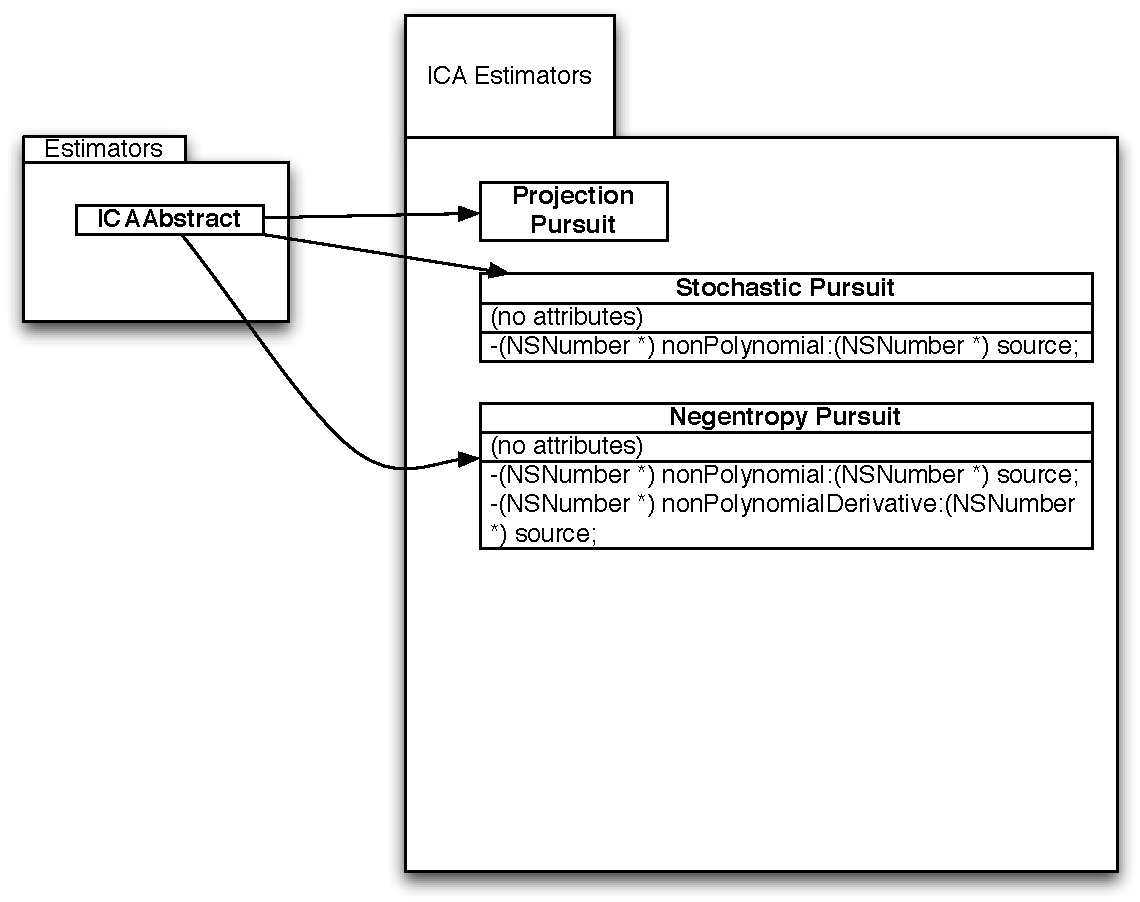
\includegraphics[width=4in]{estimators.pdf} 
   \caption{Estimators (ICA) Framework}
   \label{fig-estimator-world}
\end{figure}
%Unbiasedness and consistency
The theory of estimators is based on the Definition \ref{estimatorDefinition} and includes many linear and nonlinear methods to obtain the parameters.  % thereof.   
Estimators that achieve the estimated parameters close to the actual parameters are called constant.  
\begin{quote}
	\begin{adef}
		\label{estimatorDefinition}
	An estimator, $\hat{\mathbf{\theta}}$, of the parameter vector, $\vec{\theta}$, is the mathematical expression that estimates the parameters of an analytical solution for a given set of measurements (samples).
	\end{adef}

\cite[78]{appo-ica-book}
\end{quote}
There are a few constraints that any estimator should satisfy.   Estimators for the equations \ref{unbiasedEstimator} and \ref{unbiasedEstimatorGiven} are called unbiased.  
%Unbiased random parameters must satisfy one of the two equations: 
\begin{eqnarray}
E \{ \hat{\theta} \} \approx E \{\vec{\theta} \} \label{unbiasedEstimator}\\
E \{ \hat{\theta} | \vec{\theta} \} = \vec{\theta} \label{unbiasedEstimatorGiven}
\end{eqnarray}
Estimators not meeting this criteria are called biased.  The bias vector is defined as follows:
\begin{eqnarray}
\vec{b} = E \{ \tilde {\theta} \} \\
\vec{b} = E \{ \tilde {\theta} | \vec{\theta} \} 
\end{eqnarray}
\begin{quote}
If $\vec{b} \to \vec{0}$ as the number of measurements goes up, then the estimator is called asymmetrically unbiased.
\cite[79]{appo-ica-book}
\end{quote}

Estimators often %times 
require discrete items, which are called bins when forced on continuous values, in order to generate statistical models for data-sets.  One important concept is the loss function as defined in Definition \ref{lossFunctionDefition}
\begin{quote}
\begin{adef}
	\label{lossFunctionDefition}
A loss function $h(\tilde{\theta})$ is a metric of the relative importance of specific estimation errors.
\end{adef}
\cite[79]{appo-ica-book}
\end{quote}
%Such loss functions include invariance of bins. 
Another important concept for estimators is %their 
their metric of accuracy.  The article efficient is used as a ranking of an estimator as defined in Definition \ref{efficientEstimatorDefinition}.
%\begin{quote}
	\begin{adef}
		\label{efficientEstimatorDefinition}
An efficient estimator provides the smallest error covariance matrix among all unbiased estimators.	
	\end{adef}
\cite[81]{appo-ica-book}
%\end{quote}
Symmetry is also a means of ordering a matrix.  If $\mathbf{A}$ and $\mathbf{B}$ are both symmetrical matrices and $\mathbf{B} - \mathbf{A}$ is positive definite, then $\mathbf{A} < \mathbf{B}$.  One theorem, Cramer-Rao Lower Bound, provides for partial ordering amongst symmetric matrices.   This theorem is defined in Theorem \ref{cramerRaoLowerBound}.

%Crammer-Rao Lower Bound 
\begin{quote}
	\begin{thm}
	\label{cramerRaoLowerBound}
If $\hat{\theta}$ is any unbiased estimator of $\vec{\theta}$ based on the measurement data $\vec{x}$, then the covariance matrix of error in the estimator is bounded below by the inverse of the Fisher information matrix:
\begin{eqnarray}
J^{-1} \le E \{ (\vec{\theta} - \hat{\theta})(\vec{\theta} - \hat{\theta})^T | \vec{\theta} \} \\
J = E \{ [\frac {\partial} {\partial \vec{\theta}} \ln p(\vec{x_t} | \vec{\theta})] [\frac {\partial} {\partial \vec{\theta}} \ln p(\vec{x_t} | \vec{\theta})]^T | \vec{\theta} \}
\end{eqnarray}
	\end{thm}
\cite[83]{appo-ica-book}
\end{quote}

The last quality of an estimator is robustness.  Robustness is defined in Definition \ref{robustnessDefinition}.  Robustness determines an estimator's ability to accurately model a data-set despite the presence of outlier errors.  
\begin{quote}
	\begin{adef}
	\label{robustnessDefinition}
	Robustness is an insensitivity to gross measurement errors, and errors in specification of the parametric models.	
	\end{adef}
	\cite[83]{appo-ica-book}
\end{quote}

Maximum-likelihood (ML)  is covered in another report.  ML may be reused in the pursuit of ICA, but only in specific derivations thereof.  As this report does not cover the ML version of ICA, this report only alludes to it as an alternative estimator used to determine ICA. 

%Proofed Nov 15


\subsection{Least Squares}
Least Squares (LS) regression is a linear method used to determine specific parameters of an assumed analytical solution.  LS is a classic curve fitting method, which constructs a matrix that is solved by matrix solution methods like Gauss Jordan Elimination.
\begin{algorithm}
\caption{Least Squares Estimation (Regression) derived from definition found at \cite{wolfram-mathworld-least-squares}.}
\label{alg:least-squares}
\begin{algorithmic}
\REQUIRE DCGVector $\vec{x}$ consisting of $m$ observations
\REQUIRE Assumed model, parameters, and derived functions.
\STATE Take an initial guess at the model parameters $\lambda _i$ $\forall _i \in [1, n]$.
\REPEAT
\STATE Form matrix $A$ such that 
\begin{equation}
\left(\begin{array}{ccc}
	\frac{\partial {f(x)} } {\partial{\lambda_1}} |x_1 & ... & \frac{\partial {f(x)} } {\partial{\lambda_n }} |x_1 \\
	... & ... & ... \\
	 \frac{\partial {f(x)} } {\partial{\lambda_1}} |x_m & ... &  \frac{\partial {f(x)} } {\partial{\lambda_n}} |x_m
\end{array}\right)
\end{equation}
\STATE Compute $R = A^T A$ 
\STATE Compute $dB$ such that 
\begin{equation}
B = \sum _{i= 1} ^{m} ( y_i - f(x) )
\end{equation} 
\STATE Determine $L = A^T dB$
\STATE Determine $\partial \vec{\lambda}$ from $R(\partial {\vec{\lambda}}) = L $
\STATE Adjust $\vec{\lambda}$ by $\partial \vec{\lambda}$
\UNTIL {$d\vec{\lambda} \to 0$ }
\end{algorithmic}
\end{algorithm} 
From this algorithm, there are a family of least squares estimators.   Each one has their own assumed model and parameters.   There is a general class of LS for polynomials.   Other models such as Gaussian or other statistical models should be developed with the following rules:

	\begin{itemize}
	\item The desired property is to have more measurements than parameters (known or unknown).
	\item The goal is to choose an estimator that minimizes the effects of the error.
	\end{itemize}




\subsection{Maximum a Posteriori} 
Maximum a Posteriori (MAP) is based on Bayes Theorem, theorem \ref{bayesTheorem}.  The characteristic equation for a given set of data is the sum of a set of distributions.   Each parameter of this characteristic equation can be determined by LS regression.  This principal comes from the Optimal Estimator Theorem.  

\begin{eqnarray}
p_{\vec{\theta} | \vec{x_t}}(\vec{\theta} | \vec{x_t}) = \frac{p_{\vec{x_T} | \vec{\theta}}(\vec{x_T} | \vec{\theta}) p_{\vec{\theta}} (\vec{\theta})} { p_{\vec{x_T}} (x_T)  } \label{bayesTheorem}\\
p_{\vec{x_T}} (x_T)  = \int _{-\infty} ^{\infty} p_{\vec{x_T} | \vec{\theta}}(\vec{x_T} | \vec{\theta}) p_{\vec{\theta}} (\vec{\theta}) d\vec{\theta}
\end{eqnarray}


\begin{quote}
\begin{thm}
	\textbf{Optimal Estimator Theorem:} Assume that the parameters $\vec{\theta}$ and the observations $\vec{x_T}$ have the joint probability density function $p_{\vec{\theta} , \vec{x_t}}(\vec{\theta} , \vec{x_t})$.  The minimum mean-square estimator $\hat{\theta}_{MSE}$ of $\vec{\theta}$ is given by the conditional expectation:
\begin{equation}
\hat{\theta}_{MSE} = E[\vec{\theta} \vec{x_T}]
\end{equation}
\end{thm}
\cite[94]{appo-ica-book}
\end{quote}

The goal of MAP is to find the parameter vector $\vec{\theta}$ that maximizes the posterior density of the Bayes Theorem equation. The parameters are also based on an analytically defined model.  In this case,  $\vec{\theta}$ needs to maximize the numerator, as the denominator does not depend on $\vec{\theta}$.
\begin{eqnarray}
p_{\vec{\theta} | \vec{x_t}}(\vec{\theta} | \vec{x_t}) \approx p_{\vec{x_T} | \vec{\theta}}(\vec{x_T} | \vec{\theta}) p_{\vec{\theta}} (\vec{\theta}) d\vec{\theta} \\
\ln p_{\vec{\theta} | \vec{x_t}}(\vec{\theta} | \vec{x_t}) \approx \ln (p_{\vec{x_T} | \vec{\theta}}(\vec{x_T} | \vec{\theta}) p_{\vec{\theta}} (\vec{\theta}) d\vec{\theta}) \\
 \approx \ln( p_{\vec{x_T} | \vec{\theta}}(\vec{x_T} | \vec{\theta})) + \ln (p_{\vec{\theta}} (\vec{\theta}) d\vec{\theta} )\\
%\frac{\partial} {\partial \vec{\theta} } \ln p_{\vec{\theta} | \vec{x_t}}(\vec{\theta} | \vec{x_t}) \\ 
\approx 
\frac{\partial} {\partial \vec{\theta} } \ln( p_{\vec{x_T} | \vec{\theta}}(\vec{x_T} | \vec{\theta})) + \frac{\partial} {\partial \vec{\theta} } \ln (p_{\vec{\theta}} (\vec{\theta}) d\vec{\theta} ) \label{ln_bayes}
\end{eqnarray}


Given these equations the solution can be defined by setting equation \ref{ln_bayes} to zero.
\begin{equation}
 \frac{\partial} {\partial \vec{\theta} } \ln( p_{\vec{x_T} | \vec{\theta}}(\vec{x_T} | \vec{\theta})) + \frac{\partial} {\partial \vec{\theta} } \ln (p_{\vec{\theta}} (\vec{\theta}) d\vec{\theta} ) = 0 
\end{equation}

Like ML and EM, MAP is mentioned here as an alternative means of determining ICA.   MAP itself does not provide independent components or its mixing matrix.  Rather it provides an intermediate step from which ICA may be determined.   

\section{Entropy and Mutual Information: Determining Independence}\label{entropy}
One of the most crucial features of the ICA estimator is the ability determine independence.  Two fundamental concepts that lead to deterministic methods of independence are entropy and mutual information.  As these two concepts are very related, they are presented in the following sub-sections.

\subsection{Measures of Information}
The concept of entropy is best stated in its differential forms, both discrete and continuous.  Entropy can be treated as a measure of the amount of information contained in a specific data set.  In the discrete case, this concept can determine the minimum encoding necessary to represent the data.
\begin{eqnarray}
H(X) = \sum_i f(P(X =a_i)) \\
H(x) = - \int p_x (\eta) \log p_x (\eta) d\eta = \int f(p_x(\eta))d\eta
\end{eqnarray}
Note that transforming entropy increases and decreases monotonically. 

%The metric of mutual information between scalar random variables is 
A measure of information that one random variable has on other random variables in a set can be defined in terms of a single random variable $x_i$.  
\begin{equation}
I(\mathbf{X},\mathbf{Y})  = H(\mathbf{Y}) - H(\mathbf{Y}|\mathbf{X}) = H(\mathbf{X}) - H(\mathbf{X}|\mathbf{Y})
\end{equation}
\begin{quote}
Maximizing the joint entropy $H(Y_1, Y_2)$ is accomplished by maximizing the individual entropies while minimizing the mutual information $I(Y_1, Y_2)$.  When $I(Y_1, Y_2)$ is zero, then $Y_1$ and $Y_2$ are statistically independent.
\cite[662]{moon-stirling-book}
\end{quote}

%Neither entropy nor mutual information can be treated as a metric as there is not applicable inversion from the measure to the data.  

%\subsubsection{Kullback-Leibler Divergence}
The purpose of Kullback-Leibler Divergence is provide a pseudo metric in terms of distance  between two density functions, and therefore determine mutual information.   It is not a true metric since it is not symmetrical.   Yet, the Kullback-Leibler Divergence does increase monotonically with mutual information.  

\begin{eqnarray}
\Delta(p| q) = \sum _i p(i) (\log p(i) - \log q(i)) \\
\Delta(p| q) = \int p(i) (\log p(i) - \log q(i)) 
\end{eqnarray}


\subsection{Theory of Maximizing Representation}\label{maximizing-represnetation}

%\subsubsection{Maximum Entropy}
The goal of maximum-entropy is to determine the probability density function that satisfies equation \ref{constant-entropy} such that the $c_i$ constants are maximum.  One example under some regularity conditions is equation \ref{regularity-condition-constraint-for-entropy} (under the constraint in equation \ref{regularity-condition-constraint-for-entropy}).
\begin{eqnarray}
\int p(\eta) F_i (\eta) d\eta =  c_i \label{constant-entropy} \\
p_0( \eta) = A \exp (\sum_i a_i F_i (\eta)) \label{regularity-condition-constraint-for-entropy} \\
\int p_0 (\eta) d \eta = 1 \label{system-regularity-condition-constraint-for-entropy} 
\end{eqnarray}


\subsubsection{Negentropy}\label{maximizing-via-negentropy}
Negentropy is a concept derived from maximum entropy specifically for determining Gaussian properties.  The objective is to have ``a measure that is zero for a Gaussian variable and always nonnegative can be simply obtained from differential entropy.''  Negentropy, denoted $J(\vec{x})$, is defined in equation \ref{negentropy}.  The entropy of $x_{Gauss}$ is defined in terms the covariance matrix of $\vec{x}$ ($\Sigma$) and the dimension of $\vec{x}$.
\begin{eqnarray}
J(\vec{x}) = H(\vec{x}_{\textsl{Gauss}}) - H(\vec{x}) \label{negentropyGauss}\\
H(\vec{x}_{\textsl{Gauss}}) = \frac{1}{2}\log |\det \Sigma | + \frac{n}{2}[1 + \log {2\pi}] \label{normalEntropy}
\end{eqnarray}
Properties of negentropy include:
\begin{itemize}
	\item $J(\vec{x}) = 0$ if and only if $\vec{x}$ has a Gaussian distribution.
	\item The maximum Gaussian distribution satisfying equation \ref{constant-entropy} forces $J(\vec{x}) \ge 0$
	\item $J(\vec{x})$ is invariant and is an invertible linear transformation as proven in \cite[113]{appo-ica-book}.
\end{itemize}



\subsubsection{Approximation by Cummulants}
Polynomial density expansion approximation of negentropy, maximum entropy, and mutual information is defined for a standardized Gaussian model (zero mean and unit variance) as in equation \ref{standardized-Gaussian}, and its derivative in equation \ref{standardized-Gaussian-first-derivative}.  The polynomial system is chosen for the practicality that they are orthogonal.  
\begin{eqnarray}
\phi (\eta) = \frac{1}{2\pi} \exp (\frac{-\eta}{2}) \label{standardized-Gaussian}
\frac{\partial ^i \phi (\eta)} {\partial \eta} = (-1)^i H_i(\eta)\phi (\eta) \label{standardized-Gaussian-first-derivative}
\end{eqnarray}

Another approximation that maximizes representation is the log of the cumulants.  This approximation depends on the cumulants being relatively small.  
\begin{equation}
\log (1 + \epsilon) \approx \epsilon - \frac{\epsilon ^2}{2}
\end{equation}
Therefore, cumulants can be used to define a characteristic equation for the information carried in a data-set $x$.
\begin{eqnarray}
	p_x(\eta) \approx \phi (\eta)(1 + \kappa_3 (x) \frac{H_3(\eta)} {3!}+ \kappa_4 (x) \frac{H_4(\eta)} {4!}) \\
J(x) \approx \frac{1}{12} \kappa_3 (x) ^2 + \frac{1}{48} \kappa_4 (x) ^2
\end{eqnarray}
Thus a sum of the skewness squared and the kurtosis squared  are both computable from the random framework.  The drawback is that this method is sensitive to outliers and it measures the tails and not the center.   It is thus worth considering methods of determining entropy by non-polynomial functions.   The constraints on such methods are as follows:
%\subsubsection{Approximation of Entropy by Non-Polynomial Functions}
\begin{itemize}
\item Non-polynomial functions should be based on maximum entropy methods.
%\item Bypasses the finite expectation functions and approximations there of.  
\item Non-polynomial functions confine the distribution from the infinite  which will satisfy to a specific set of constraints.  
%\item Called the maximum entropy method, it is a ``first order approximation'' for a continuous one-dimensional random variable.  
\end{itemize}






\bibliography{../../patternNotes.bib}
\bibliographystyle{abbrv}
\end{document}  